\documentclass[UKenglish,oneside]{memoir}

\bibliographystyle{plainurl}

\usepackage{ifxetex}

\ifxetex
  \usepackage{polyglossia}
  \usepackage{fontspec}

  \setmainlanguage{english}
\else
  \usepackage[english]{babel}
\fi

\usepackage{marvosym}
\usepackage{hyperref}
\usepackage{blindtext}
\usepackage{graphicx}
\usepackage{tabularx}
\usepackage{listings}
\usepackage{tikz}
\usepackage{pifont}
\usepackage{fontawesome}
\usepackage{tikzpeople}
\usepackage{upquote}
\usepackage{tikzsymbols}
\usepackage{bookmark}
\usepackage{printlen}
\usepackage{xcolor}
\usepackage[fleqn]{mathtools}
\usepackage{amssymb}
\usepackage[fleqn]{amsmath}
\usepackage[h]{esvect}
\usepackage{multicol}

\usetikzlibrary{arrows, arrows.meta, decorations.markings, shapes, calc, positioning, fit, graphs, trees, matrix, backgrounds, bending, decorations.pathmorphing, decorations.pathreplacing, decorations.shapes, fadings, shadings, patterns, graphs.standard, patterns.meta}

%Page style
% \geometry{
% left=16mm,
% top=30mm,
% right=16mm,
% bottom=30mm
% }

\linespread{1.1}

\pagestyle{headings}

\setlength{\columnseprule}{0pt}
\setlength\columnsep{10pt}

\newcommand\blankpage{%
    \null
    \thispagestyle{empty}%
    \addtocounter{page}{-1}%
    \newpage}

%Chapter style

\makechapterstyle{box}{
  \renewcommand*{\printchaptername}{}
  \renewcommand*{\chapnumfont}{\normalfont\sffamily\huge\bfseries}
  \renewcommand*{\printchapternum}{
    \flushright
    \begin{tikzpicture}
      \draw[fill,color=black] (0,0) rectangle (2cm,2cm);
      \draw[color=white] (1cm,1cm) node { \chapnumfont\thechapter };
    \end{tikzpicture}
  }
  \renewcommand*{\chaptitlefont}{\normalfont\sffamily\Huge\bfseries}
  \renewcommand*{\printchaptertitle}[1]{\flushright\chaptitlefont##1}
}
\chapterstyle{box}

%Section style
\renewcommand\secheadstyle{\centering\Large\scshape\noindent}

%Page style
% \geometry{
% left=3.2cm,
% top=2.5cm,
% right=2.5cm,
% bottom=2.5cm
% }

% \setlrmarginsandblock{2.5cm}{2.5cm}{*}
% \setulmarginsandblock{3.5cm}{3cm}{*}
% % \setlrmarginsandblock{3cm}{2cm}{*}
% % \setulmarginsandblock{3cm}{2cm}{*}
% \checkandfixthelayout

% \setbeforesubparaskip{1.5ex plus 1ex minus .2ex} % default : 3.25ex plus 1ex minus .2ex
% \setsubparaindent{0pt}

% \setlength{\headwidth}{\textwidth}
% \makerunningwidth{companion}{\headwidth}

\chapterstyle{madsen} % veelo
\pagestyle{companion} % ruled, Ruled

\setsecnumdepth{subsection}

\firmlists*

\definecolor{bordeau}{rgb}{0.3515625,0,0.234375}
\definecolor{lipiyellow}{rgb}{0.99,0.78,0.07}
\definecolor{tileblue}{rgb}{0.30,0.62,0.80}
\definecolor{checkgreen}{rgb}{0.0,0.7,0.0}


\linespread{1.05}

\pagestyle{headings}

\setsecnumdepth{subsection}

\setlength{\columnseprule}{0pt}
\setlength\columnsep{10pt}

% \newcommand\blankpage{%
%     \null
%     \thispagestyle{empty}%
%     \addtocounter{page}{-1}%
%     \newpage}

% Hyperref customization
\hypersetup{
  colorlinks,
  linkcolor={red!70!black},
  citecolor={blue!70!black},
  urlcolor={blue!80!black}
}


%Chapter style
\makechapterstyle{box}{
  \renewcommand*{\printchaptername}{}
  \renewcommand*{\chapnumfont}{\normalfont\sffamily\huge\bfseries}
  \renewcommand*{\printchapternum}{
    \flushright
    \begin{tikzpicture}
      \draw[fill,color=black] (0,0) rectangle (2cm,2cm);
      \draw[color=white] (1cm,1cm) node { \chapnumfont\thechapter };
    \end{tikzpicture}
  }
  \renewcommand*{\chaptitlefont}{\normalfont\sffamily\Huge\bfseries}
  \renewcommand*{\printchaptertitle}[1]{\flushright\chaptitlefont##1}
}
\chapterstyle{box}

%Section style
\renewcommand\secheadstyle{\centering\Large\scshape\noindent}

%Subappendices
\AtBeginEnvironment{subappendices}{%
\renewcommand\thesection{A$_{\text{\thechapter}}$}
\section{Appendix of \chaptername~\thechapter}
\counterwithin{figure}{section}
\counterwithin{table}{section}
}
\AtEndEnvironment{subappendices}{%
\counterwithout{figure}{section}
\counterwithin{figure}{chapter}
\counterwithout{table}{section}
\counterwithin{table}{chapter}
}

\newcommand{\refappendix}[1]{Appendix~\ref{#1}}

%Intext labels
\makeatletter
\def\intextlabel#1#2#3#4{%
  \begin{#4}%
  #1%
  \begingroup%
    \def\@currentlabel{\normalfont{(#2)}}%
    \phantomsection\label{#3}%
  \endgroup%
  \end{#4}%
}
\makeatother

\newenvironment{lab-dot-env}{}{.\,}
\newenvironment{lab-par-env}{(}{)}
\newenvironment{lab-emp-env}{}{}

\makeatletter
\def\phantomlabel#1#2{\begingroup
   \def\@currentlabel{#1}%
   \label{#2}\endgroup
}
\makeatother

\newcommand{\itemlabel}[2]{\intextlabel{#1}{#1}{#2}{lab-dot-env}}
\newcommand{\parenthesislabel}[2]{\intextlabel{#1}{#1}{#2}{lab-par-env}}
\newcommand{\emptylabel}[2]{\intextlabel{}{#1}{#2}{lab-emp-env}}

\newcommand{\highitem}[1]{\normalfont{\textit{#1.}}}

%Axioms labels 

\newcommand{\preaxiomlab}[2]{\intextlabel{#1}{#1}{#2}{lab-par-env}}

\newcommand{\axlab}[2]{\preaxiomlab{%
    \textbf{${#1}_{\number\numexpr\value{enumi}+1}$}%
  }{#2}\setcounter{enumi}{\number\numexpr\value{enumi}+1}}

% \makeatletter
% \def\axlab#1#2{%
%   \textbf{($\mathbf{#1_{\number\numexpr\value{enumi}+1}}$)}%
%   \begingroup%
%     \def\@currentlabel{\textbf{($\mathbf{#1_{\number\numexpr\value{enumi}+1}}$)}}%
%     \phantomsection\label{#2}%
%   \endgroup%
%   \setcounter{enumi}{\number\numexpr\value{enumi}+1}%
% }
% \makeatother

\makeatletter
\def\indexedlab#1#2#3{%
  \textbf{($\mathbf{#1_{#2.\number\numexpr\value{enumi}+1}}$)}%
  \begingroup%
    \def\@currentlabel{\textbf{($\mathbf{#1_{#2.\number\numexpr\value{enumi}+1}}$)}}%
    \phantomsection\label{#3}%
  \endgroup%
  \setcounter{enumi}{\number\numexpr\value{enumi}+1}%
}
\makeatother

\makeatletter
\def\rulelab#1#2{%
  \ \ #1:%
  \begingroup%
    \def\@currentlabel{#1}%
    \phantomsection\label{#2}%
  \endgroup%
}
\makeatother

\makeatletter
\def\lemmalab#1#2{%
  \ \ {\textbf{#1}}%
  \begingroup%
    \def\@currentlabel{\textbf{#1}}%
    \phantomsection\label{#2}%
  \endgroup%
}
\makeatother

%Syntactical proofs 

\newenvironment{syntproof}
  {
  \begin{tcenter}
    \def\arraystretch{1.4}
    \setlength\LTleft{\textwidth-\linewidth}
    \setlength\LTright{0pt}
    \noindent%
    \begin{longtable}{L|M@{\extracolsep{\fill}}M}
    }
    { 
    \end{longtable}
  \end{tcenter}
  }

\newenvironment{smallsyntproof}
  {
  \begin{tcenter}
    \def\arraystretch{1.4}
    \noindent%
    \begin{tabular*}{1\linewidth}{L|M@{\extracolsep{\fill}}M}
    }
    { 
    \end{tabular*}
  \end{tcenter}
  }


\newcommand{\elseabsurd}[2]{\textbf{By}\ #1\ \textbf{it holds that}\ #2\textbf{$_{\blacksquare}$}}
   

%TOC style
  %TOC - Part
  \renewcommand\cftpartaftersnum{\space}
  \setlength{\cftpartnumwidth}{3em}% Width of \part numbers in ToC
  \renewcommand{\cftpartpresnum}{\hfill}% Inserted before \part numbers in ToC
  \renewcommand{\cftpartaftersnum}{\quad}% Inserts after \part numbers in ToC

  %TOC - Chapter
  \renewcommand\cftchapteraftersnum{.\space}
  \setlength{\cftchapternumwidth}{3em}
  \renewcommand{\cftchapterpresnum}{\hfill}
  \renewcommand{\cftchapteraftersnum}{\quad}

  %TOC - Section
  \setlength{\cftsectionnumwidth}{3em}
  \renewcommand{\cftsectionpresnum}{\hfill}
  \renewcommand{\cftsectionaftersnum}{\quad}

%Rule environments
\newenvironment{rfigure}{%
    \begin{figure}[t]
    \hrule
    \vspace{4pt}
    \centering
    \def\arraystretch{1.5}
}
{
\vspace{2pt}
\hrule
\end{figure}%
}

\newenvironment{bigfigure}{%
    \begin{figure}
    \hrule
    \vspace{4pt}
    \centering
    \def\arraystretch{1.5}
}
{
\vspace{2pt}
\hrule
\end{figure}%
}

\newenvironment{rtable}{%
    \begin{table}
    \hrule
    \vspace{4pt}
}
{
\hrule
\end{table}%
}

%Multicols spacing
\setlength{\multicolsep}{6.0pt plus 2.0pt minus 1.5pt}% 50% of original values

%Centering macros
\newenvironment{tcenter}
  {%
    \setlength{\topsep}{0.85\topsep}\par\kern\topsep\centering%
  }
  {%
    \par\kern\topsep%
  }

%Roman numbers
\makeatletter
\newcommand*{\rom}[1]{\expandafter\@slowromancap\romannumeral #1@}
\makeatother

%Tabular spacing
\def\arraystretch{1.2}
\setlength{\tabcolsep}{5pt}

%Math Text Style
\newcommand{\mathfont}[1]{\mathsf{#1}}

%Big Operations
\makeatletter
\DeclareRobustCommand\bigop[1]{%
  \mathop{\vphantom{\sum}\mathpalette\bigop@{#1}}\slimits@
}
\newcommand{\bigop@}[2]{%
  \vcenter{%
    \sbox\z@{$#1\sum$}%
    \hbox{\resizebox{\ifx#1\displaystyle.9\fi\dimexpr\ht\z@+\dp\z@}{!}{$\m@th#2$}}%
  }%
}
\makeatother


\tikzset{
  align=center,
  node distance=1.5cm,
  dot/.style={draw, minimum size=1.4mm, inner sep=0pt, outer sep=0pt, shape=circle, fill=black},
  pto/.style={-{latex},thick},
  bordeaupto/.style={-{latex},very thick,bordeau},
  highlightpath/.style={draw,line width=5pt,-,lipiyellow},
  highlightnode/.style={dot,fill=black,minimum size=1.6mm,draw=lipiyellow,line width=1.1pt},
  aloc/.style={inner sep=0pt, outer sep=0pt, minimum size=1.4mm, draw=black, fill=white},
  curly/.style={decorate,decoration={brace,amplitude=8pt},xshift=4pt,yshift=5pt},
  snaky/.style={decorate, decoration={snake, amplitude=0.2mm, segment length=2mm, post length=0.5mm},shorten >=1pt},
  reach/.style={snaky,pto},
  segment/.style={|-|,line width=0.25mm,black!90},
  alin/.style={line width=0.25mm,black!90},
  aux/.style={-latex,line width=0.25mm,black!80},
  path/.style={-latex,dashed,line width=0.28mm,dash pattern=on 7pt off 3pt on 3pt off 3pt on 3pt off 3pt on 3pt off 3pt}
}


% \faculty{Faculty of Computer Science}
% \institute{Institute of Theoretical Computer Science}
% \chair{Computational Logic}
\date{12.04.2024}
\author{Benno Fünfstück}
\title{A constructive proof of a van~Benthem Theorem for the Forward Guarded Fragment of First Order Logic}
% \subject{master}
\newcommand{\supervisor}{Bartosz Bednarczyk}
\newcommand{\refereeFst}{Prof. Dr. Sebastian Rudolph}
\newcommand{\refereeSnd}{Dr.-Ing. Stefan Borgwardt}
% \referee{Prof. Dr. Sebastian Rudolph \and Dr.-Ing. Stefan Borgwardt}

% Inline comments
\definecolor{ao(english)}{rgb}{0.0, 0.5, 0.0}
\definecolor{brickred}{rgb}{0.8, 0.25, 0.33}
\newcommand{\myundef}[1]{\textcolor{brickred}{\textbf{#1}}}
\newcommand{\possiblelie}[1]{\textcolor{brickred}{\textbf{#1}}}
\newcommand{\becareful}[1]{\textcolor{brickred}{\textbf{#1}}}
\newcommand{\bennof}[1]{\textbf{\textcolor{blue}{\textbf{#1}}}}
\newcommand{\bbe}[1]{\textbf{\textcolor{ao(english)}{#1}}}
\newcommand{\bbebox}[1]{\todo[inline,color=green!30]{\textbf{BB\@: }#1}\xspace}
\newcommand{\bbeside}[1]{\todo[color=green!30,size=\scriptsize,fancyline]{\textbf{BB\@: }#1}\xspace}
\newcommand{\bfbox}[1]{\todo[inline,color=blue!30]{\textbf{BF\@: }#1}\xspace}
\newcommand{\bfside}[1]{\todo[color=blue!30,size=\scriptsize,fancyline]{\textbf{BF\@: }#1}\xspace}

% logics:
\newcommand{\Logic}[1]{\ensuremath{\mathsf{#1}}} % a Logic
\newcommand{\logicL}{\Logic{L}} % some logic L
\newcommand{\Laffix}{\Logic{L}_{\mathsf{affix}}}   % L_affix
\newcommand{\Linfix}{\Logic{L}_{\mathsf{inf}}}   % L_infix
\newcommand{\Lsuffix}{\Logic{L}_{\mathsf{suf}}} % L_suffix
\newcommand{\Lprefix}{\Logic{L}_{\mathsf{pre}}} % L_prefix

\newcommand{\Gaffix}{\Logic{G}_{\mathsf{affix}}}   % G_affix
\newcommand{\Ginfix}{\Logic{G}_{\mathsf{inf}}}     % G_infix
\newcommand{\Gsuffix}{\Logic{G}_{\mathsf{suf}}}    % G_suffix
\newcommand{\Gprefix}{\Logic{G}_{\mathsf{pre}}}    % G_prefix

\newcommand{\GF}{\Logic{GF}}   % Guarded Fragment
\newcommand{\FGF}{\Logic{FGF}}   % Forward Guarded Fragment
\newcommand{\FO}{\Logic{FO}}   % First-Order Logic

% Complexity classses:
\newcommand{\complexityclass}[1]{\textsc{#1}} % any complexity class
\newcommand{\ExpTime}{\complexityclass{ExpTime}} % exponential time
\hyphenation{Exp-Time} % prevent "Ex-PTime" (see, e.g. Tobies'01, Glimm'07 ;-)
\newcommand{\NExpTime}{\complexityclass{NExpTime}} % nondeterministic exponential time
\hyphenation{NExp-Time} % prevent "Ex-PTime" (see, e.g. Tobies'01, Glimm'07 ;-)
\newcommand{\TwoExpTime}{\complexityclass{2ExpTime}} % doubly-exponential time
\newcommand{\TwoNExpTime}{\complexityclass{2NExpTime}} % doubly-nondeterministic-exponential time
\newcommand{\coNExpTime}{\complexityclass{coNExpTime}} % co nondeterministic exponential time
\hyphenation{coNExp-Time} 
\newcommand{\Tower}{\complexityclass{Tower}}
\newcommand{\LogSpace}{\complexityclass{LogSpace}}
\newcommand{\PSpace}{\complexityclass{PSpace}}
\newcommand{\PTime}{\complexityclass{PTime}}

% Others
\newcommand{\str}[1]{{\mathfrak{#1}}}
\DeclareRobustCommand{\unravel}[1]{\vv{\mathfrak{#1}}}
\newcommand{\deff}{\coloneqq}
\newcommand{\arity}{\mathsf{ar}}
\renewcommand{\iff}{\leftrightarrow}

\newcommand{\N}{{\mathbb{N}}}
\newcommand{\Z}{{\mathbb{Z}}} 
\newcommand{\Q}{{\mathbb{Q}}}
\newcommand{\V}{\mathbf{V}} 
\newcommand{\R}{\mathbf{R}} 
\newcommand{\Var}{\mathrm{Var}}
\newcommand{\sigSigma}{\Sigma}

\newcommand{\sqin}{%
  \mathrel{\vphantom{\sqsubset}\text{%
    \mathsurround=0pt
    \ooalign{$\sqsubset$\cr$-$\cr}%
  }}%
}

% Rel symbols
\newcommand{\rel}[1]{\mathrm{#1}}
\newcommand{\relP}{\rel{P}}
\newcommand{\relR}{\rel{R}}
\newcommand{\relQ}{\rel{Q}}
\newcommand{\relS}{\rel{S}}
\newcommand{\relT}{\rel{T}}
\newcommand{\relU}{\rel{U}}
\newcommand{\relA}{\rel{A}}
\newcommand{\relB}{\rel{B}}
\newcommand{\relC}{\rel{C}}
\newcommand{\relD}{\rel{D}}
\newcommand{\relE}{\rel{E}}
\newcommand{\relH}{\rel{H}}
\newcommand{\sig}{\mathsf{sig}}

% Tuples 
\newcommand{\emptytupl}{\varepsilon}
\newcommand{\set}{\mathsf{set}}

% Domain elements
\newcommand{\elem}[1]{\mathrm{#1}}                           % domain element
\newcommand{\elema}{\elem{a}}                             % domain element a
\newcommand{\elemb}{\elem{b}}                             % domain element b
\newcommand{\elemc}{\elem{c}}                             % domain element c
\newcommand{\elemd}{\elem{d}}                             % domain element d
\newcommand{\eleme}{\elem{e}}                             % domain element e
\newcommand{\elemf}{\elem{f}}                               % domain element f
\newcommand{\elemg}{\elem{g}}                             % domain element g
\newcommand{\elemh}{\elem{h}}                             % domain element h
\newcommand{\elemi}{\elem{i}}                             % domain element i
\newcommand{\elemj}{\elem{j}}                             % domain element j
\newcommand{\elemo}{\elem{o}}                             % domain element o
\newcommand{\elemp}{\elem{p}}                             % domain element p
\newcommand{\elemq}{\elem{q}}                             % domain element q
\newcommand{\elemr}{\elem{r}}                             % domain element r
\newcommand{\elems}{\elem{s}}                             % domain element s
\newcommand{\elemt}{\elem{t}}                             % domain element t
\newcommand{\elemw}{\elem{w}}                             % domain element w
\newcommand{\elemv}{\elem{v}}                             % domain element v
\newcommand{\elemu}{\elem{u}}                             % domain element u
\newcommand{\elemx}{\elem{x}}                             % domain element u
\newcommand{\elemtuplea}{\overline{\elema}}                         % tuple of domain element a
\newcommand{\elemtupleb}{\overline{\elemb}}                         % tuple of domain element b
\newcommand{\elemtuplec}{\overline{\elemc}}                         % tuple of domain element c
\newcommand{\elemtupled}{\overline{\elemd}}                         % tuple of domain element d
\newcommand{\elemtuplee}{\overline{\eleme}}                         % tuple of domain element e
\newcommand{\elemtuplef}{\overline{\elemf}}                           % tuple of domain element f
\newcommand{\elemtupleg}{\overline{\elemg}}                         % tuple of domain element g
\newcommand{\elemtupleh}{\overline{\elemh}}                         % tuple of domain element h
\newcommand{\elemtuplei}{\overline{\elemi}}                         % tuple of domain element i
\newcommand{\elemtupleo}{\overline{\elemo}}                         % tuple of domain element o
\newcommand{\elemtuplep}{\overline{\elemp}}                         % tuple of domain element p
\newcommand{\elemtupleq}{\overline{\elemq}}                         % tuple of domain element q
\newcommand{\elemtupler}{\overline{\elemr}}                         % tuple of domain element r
\newcommand{\elemtuples}{\overline{\elems}}                         % tuple of domain element s
\newcommand{\elemtuplet}{\overline{\elemt}}                         % tuple of domain element t
\newcommand{\elemtuplew}{\overline{\elemw}}                         % tuple of domain element w
\newcommand{\elemtupleu}{\overline{\elemu}}                         % tuple of domain element u
\newcommand{\elemtuplev}{\overline{\elemv}}                         % tuple of domain element v
\newcommand{\elemtuplex}{\overline{\elemx}}                         % tuple of domain element v

\newcommand{\elemtupledfromto}[2]{\overline{\elemd}_{#1\ldots#2}}  % tuple of domelements d from #1 to #2
\newcommand{\elemtupleefromto}[2]{\overline{\eleme}_{#1\ldots#2}}  % tuple of domelements e from #1 to #2
\newcommand{\elemtuplecfromto}[2]{\overline{\elemc}_{#1\ldots#2}}  % tuple of domelements c from #1 to #2
\newcommand{\elemtuplebfromto}[2]{\overline{\elemb}_{#1\ldots#2}}  % tuple of domelements b from #1 to #2
\newcommand{\elemtupleafromto}[2]{\overline{\elema}_{#1\ldots#2}}  % tuple of domelements a from #1 to #2
\newcommand{\elemtupleffromto}[2]{{\elemtuplef}_{#1\dots#2}} % tuple of domelements f from #1 to #2
\newcommand{\elemtuplegfromto}[2]{{\elemtupleg}_{#1\dots#2}} % tuple of domelements g from #1 to #2

\DeclareRobustCommand{\elemtuptuplea}{\vv{\elema}}                         % tuple of domain element a
\DeclareRobustCommand{\elemtuptupleb}{\vv{\elemb}}                         % tuple of domain element b
\DeclareRobustCommand{\elemtuptuplec}{\vv{\elemc}}                         % tuple of domain element c
\DeclareRobustCommand{\elemtuptupled}{\vv{\elemd}}                         % tuple of domain element d
\DeclareRobustCommand{\elemtuptuplee}{\vv{\eleme}}                         % tuple of domain element e
\DeclareRobustCommand{\elemtuptuplef}{\vv{\elemf}}                           % tuple of domain element f
\DeclareRobustCommand{\elemtuptupleg}{\vv{\elemg}}                         % tuple of domain element g
\DeclareRobustCommand{\elemtuptupleh}{\vv{\elemh}}                         % tuple of domain element h
\DeclareRobustCommand{\elemtuptuplei}{\vv{\elemi}}                         % tuple of domain element i
\DeclareRobustCommand{\elemtuptuplej}{\vv{\elemj}}                         % tuple of domain element j
\DeclareRobustCommand{\elemtuptuplep}{\vv{\elemp}}                         % tuple of domain element p
\DeclareRobustCommand{\elemtuptupleq}{\vv{\elemq}}                         % tuple of domain element q
\DeclareRobustCommand{\elemtuptupler}{\vv{\elemr}}                         % tuple of domain element r
\DeclareRobustCommand{\elemtuptuples}{\vv{\elems}}                         % tuple of domain element s
\DeclareRobustCommand{\elemtuptuplet}{\vv{\elemt}}                         % tuple of domain element t
\DeclareRobustCommand{\elemtuptuplew}{\vv{\elemw}}                         % tuple of domain element w
\DeclareRobustCommand{\elemtuptupleu}{\vv{\elemu}}                         % tuple of domain element u
\DeclareRobustCommand{\elemtuptuplev}{\vv{\elemv}}                         % tuple of domain element v
\DeclareRobustCommand{\elemtuptuplex}{\vv{\elemx}}                         % tuple of domain element v

% Variables:
\newcommand{\var}[1]{\mathit{#1}}       % variable
\newcommand{\varx}{\var{x}}             % variable x
\newcommand{\vary}{\var{y}}             % variable y
\newcommand{\varz}{\var{z}}             % variable z
\newcommand{\varv}{\var{v}}             % variable v
\newcommand{\varu}{\var{u}}             % variable u
\newcommand{\varw}{\var{w}}             % variable w
\newcommand{\varh}{\var{h}}             % variable h
\newcommand{\vartuplex}{\overline{\varx}}    % tuple of variables x
\newcommand{\vartuplexomega}{\overline{\varx_{\omega}}}      % tuple of variables x_omega
\newcommand{\vartupley}{\overline{\vary}}                    % tuple of variables y
\newcommand{\vartupleyone}{\overline{\vary_1}}                    % tuple of variables y_1
\newcommand{\vartupleytwo}{\overline{\vary_2}}                    % tuple of variables y_2
\newcommand{\vartuplez}{\overline{\varz}}                    % tuple of variables z
\newcommand{\vartuplev}{\overline{\varv}}                    % tuple of variables v
\newcommand{\vartupleu}{\overline{\varu}}                    % tuple of variables u
\newcommand{\vartuplew}{\overline{\varw}}                    % tuple of variables w
\newcommand{\vartupleh}{\overline{\varh}}                    % tuple of variables h
\newcommand{\vartuplexfromto}[2]{\overline{\varx}_{#1\ldots#2}}  % tuple of variables x from #1 to #2
\newcommand{\vartupleyfromto}[2]{\overline{\vary}_{#1\ldots#2}}  % tuple of variables y from #1 to #2
\newcommand{\vartupleufromto}[2]{\overline{\varu}_{#1\ldots#2}}  % tuple of variables u from #1 to #2
\newcommand{\vartuplevfromto}[2]{\overline{\varv}_{#1\ldots#2}}  % tuple of variables v from #1 to #2
\newcommand{\vartuplewfromto}[2]{\overline{\varw}_{#1\ldots#2}}  % tuple of variables v from #1 to #2

% Theory
\newcommand{\theory}[1]{\mathcal{#1}}   % theory
\newcommand{\theoryT}{\theory{T}}       % theory T

% Types
\newcommand{\atp}[3]{\mathsf{atp}^{#1}_{#2}(#3)}
\newcommand{\tp}[3]{\mathsf{tp}^{#1}_{#2}(#3)}

% Tree unravelings
\newcommand{\seq}[1]{\mathsf{seq}(#1)}
\newcommand{\ctr}[1]{\mathsf{ctr}(#1)}
\newcommand{\bound}[1]{\mathsf{bnd}(#1)}
\newcommand{\relNext}{\rel{Next}}
\newcommand{\unraveldom}[1]{\vv{#1}}
\newcommand{\Seq}[1]{\mathsf{Seq}(\str{#1})}
\newcommand{\hist}[2]{\mathsf{hist}_{#1}(#2)}

% Restrictions
\renewcommand{\restriction}{\mathord{\upharpoonright}}
\newcommand{\restr}[2]{#1\restriction_{#2}} % the restriction of #1 to #2

% morphisms
\newcommand{\homo}[1]{\mathfrak{#1}}    % homomorphism
\newcommand{\homof}{\homo{f}}           % homomorphism f
\newcommand{\homog}{\homo{g}}           % homomorphism g
\newcommand{\homoh}{\homo{h}}           % homomorphism h
\newcommand{\homop}{\homo{p}}           % homomorphism p
\newcommand{\homoe}{\homo{e}}           % homomorphism e
\newcommand{\ishomoto}{\vartriangleleft} % is homomorhic to
\newcommand{\homeq}{\rightleftarrows} % homomorphically equivalent
\newcommand{\isoeq}{\cong} % isomorphic
\newcommand{\elemext}{\preceq} % elementary extension
\newcommand{\omegasat}[1]{\widehat{#1}}
\newcommand{\partisof}{\homo{f}}           % partial isomorphism f
\newcommand{\partisog}{\homo{g}}           % partial isomorphism g
\newcommand{\partisoh}{\homo{h}}           % partial isomorphism h

% bisimulations
\newcommand{\bisimulation}[1]{\mathcal{#1}} % a bisimulation
\newcommand{\bisimY}{\bisimulation{Y}}
\newcommand{\bisimZ}{\bisimulation{Z}}
\newcommand{\bisimto}{\sim} % bisimilarity relation
\newcommand{\strbisimto}{\approx} % strong bisimilarity relation
\newcommand{\PartIso}[2]{\mathsf{Part}(#1,#2)}

% tikz helpers
\newcommand{\tikzdbg}{%
  \draw[step=5em,color=lightgray]%
    (current bounding box.south west) grid (0,0)%
    (current bounding box.north west) grid (0,0)%
    (current bounding box.south east) grid (0,0)%
    (current bounding box.north east) grid (0,0);%
  \fill[red] (0,0) circle (0.1);%
}

% Proof sketchs
\let\realproof\proof
\let\realendproof\endproof
% \newenvironment{proofsketch}{%
%   \renewcommand{\proofname}{\normalfont\emph{Proof Sketch}}\realproof}{\realendproof}

% hide proofs
\let\proof\appendixproof
\let\endproof\endappendixproof

% Macros for compatibility with lipics class
\def\romanenumerate{\enumerate[(i)]}
\let\endromanenumerate\endenumerate

\definecolor{tolbrightBlue}{HTML}{4477AA}
\definecolor{tolbrightRed}{HTML}{EE6677}
\definecolor{tolbrightGreen}{HTML}{228833}
\definecolor{tolbrightYellow}{HTML}{CCBB44}
\colorlet{tolbrightYellowDarker}{tolbrightYellow!70!black}
\definecolor{tolbrightCyan}{HTML}{66CCEE}
\colorlet{tolbrightCyanDarker}{tolbrightCyan!70!black}
\definecolor{tolbrightPurple}{HTML}{AA3377}
\definecolor{tolbrightGrey}{HTML}{BBBBBB}
\definecolor{tolhighcontrastBlue}{HTML}{004488}
\definecolor{tolhighcontrastYellow}{HTML}{DDAA33}
\definecolor{tolhighcontrastRed}{HTML}{BB5566}
\definecolor{tolvibrantOrange}{HTML}{EE7733}
\definecolor{tolvibrantBlue}{HTML}{0077BB}
\definecolor{tolvibrantCyan}{HTML}{33BBEE}
\definecolor{tolvibrantMagenta}{HTML}{EE3377}
\definecolor{tolvibrantRed}{HTML}{CC3311}
\definecolor{tolvibrantTeal}{HTML}{009988}
\definecolor{tolvibrantGrey}{HTML}{BBBBBB}
\definecolor{tolmutedRose}{HTML}{CC6677}
\definecolor{tolmutedIndigo}{HTML}{332288}
\definecolor{tolmutedSand}{HTML}{DDCC77}
\definecolor{tolmutedGreen}{HTML}{117733}
\definecolor{tolmutedCyan}{HTML}{88CCEE}
\definecolor{tolmutedWine}{HTML}{882255}
\definecolor{tolmutedTeal}{HTML}{44AA99}
\definecolor{tolmutedOlive}{HTML}{999933}
\definecolor{tolmutedPurple}{HTML}{AA4499}
\definecolor{tolmutedPalegrey}{HTML}{DDDDDD}
\definecolor{tolmediumcontrastLightblue}{HTML}{6699CC}
\definecolor{tolmediumcontrastDarkblue}{HTML}{004488}
\definecolor{tolmediumcontrastLightyellow}{HTML}{EECC66}
\definecolor{tolmediumcontrastDarkred}{HTML}{994455}
\definecolor{tolmediumcontrastDarkyellow}{HTML}{997700}
\definecolor{tolmediumcontrastLightred}{HTML}{EE99AA}
\definecolor{tolpalePaleblue}{HTML}{BBCCEE}
\definecolor{tolpalePalered}{HTML}{FFCCCC}
\definecolor{tolpalePalegreen}{HTML}{CCDDAA}
\definecolor{tolpalePaleyellow}{HTML}{EEEEBB}
\definecolor{tolpalePalecyan}{HTML}{CCEEFF}
\definecolor{tolpalePalegrey}{HTML}{DDDDDD}
\definecolor{toldarkDarkblue}{HTML}{222255}
\definecolor{toldarkDarkred}{HTML}{663333}
\definecolor{toldarkDarkgreen}{HTML}{225522}
\definecolor{toldarkDarkyellow}{HTML}{666633}
\definecolor{toldarkDarkcyan}{HTML}{225555}
\definecolor{toldarkDarkgrey}{HTML}{555555}
\definecolor{tollightLightblue}{HTML}{77AADD}
\definecolor{tollightOrange}{HTML}{EE8866}
\definecolor{tollightLightyellow}{HTML}{EEDD88}
\definecolor{tollightPink}{HTML}{FFAABB}
\definecolor{tollightLightcyan}{HTML}{99DDFF}
\definecolor{tollightMint}{HTML}{44BB99}
\definecolor{tollightPear}{HTML}{BBCC33}
\definecolor{tollightOlive}{HTML}{AAAA00}
\definecolor{tollightPalegrey}{HTML}{DDDDDD}

% Proof sketchs
% \let\realproof\proof
% \let\realendproof\endproof
% \newenvironment{proofsketch}{%
%   \renewcommand{\proofname}{\normalfont\emph{Proof Sketch}}\realproof}{\realendproof}

% hide proofs
% \let\proof\appendixproof
% \let\endproof\endappendixproof

% \newtheorem{theorem}{Theorem}
% \newtheorem{lemma}[theorem]{Lemma}
% \newtheorem{corollary}[theorem]{Corollary}
% \newtheorem{proposition}[theorem]{Proposition}
% \newtheorem{exercise}[theorem]{Exercise}
% \newtheorem{definition}[theorem]{Definition}
% \newtheorem{conjecture}[theorem]{Conjecture}
% \newtheorem{observation}[theorem]{Observation}
% \theoremstyle{definition}
% \newtheorem{example}[theorem]{Example}
% \theoremstyle{remark}
% \newtheorem{note}[theorem]{Note}
% \newtheorem*{note*}{Note}
% \newtheorem{remark}[theorem]{Remark}
% \newtheorem*{remark*}{Remark}
% \theoremstyle{claimstyle}
% \newtheorem{claim}[theorem]{Claim}
% \newtheorem*{claim*}{Claim}


\newcommand{\problemdef}[4]{
  \smallskip
\begin{center}
\begin{tabular}{|r p{36em} |}
  \hline
\multicolumn{2}{|l|}{\rule{0pt}{2.6ex}\textbf{#1}} \\[.12ex]
\textit{Parameters:}     & #2\\[.12ex]
\textit{Input:}     & #3\\[.12ex]
\textit{Question:}  & #4 \\[.12ex]
\hline
\end{tabular}
\end{center}
\smallskip
}

\newcommand{\problemdeff}[3]{
  \smallskip
\begin{center}
\begin{tabular}{|r p{36em} |}
  \hline
\multicolumn{2}{|l|}{\rule{0pt}{2.6ex}\textbf{#1}} \\[.12ex]
\textit{Input:}     & #2\\[.12ex]
\textit{Question:}  & #3 \\[.12ex]
\hline
\end{tabular}
\end{center}
\smallskip
}


\definecolor{ForestGreen}{RGB}{34,139,34}
\definecolor{Salmon}{rgb}{1.0, 0.55, 0.41}
\definecolor{RawSienna}{rgb}{0.77, 0.12, 0.23}% \definecolor{carminered}{rgb}
\definecolor{MidnightBlue}{rgb}{0.0, 0.2, 0.4}
\definecolor{RedViolet}{rgb}{0.78, 0.08, 0.52}
\definecolor{TealBlue}{rgb}{0.21, 0.46, 0.53}
\definecolor{brandeisblue}{rgb}{0.0, 0.44, 1.0}

%%fakesection Theorems

\theoremstyle{definition}
\mdfdefinestyle{mdbluebox}{%
  roundcorner = 10pt,
  linewidth=1pt,
  skipabove=12pt,
  innerbottommargin=9pt,
  skipbelow=2pt,
  nobreak=true,
  linecolor=blue,
  backgroundcolor=TealBlue!8,
}
\declaretheoremstyle[
  headfont=\sffamily\bfseries\color{MidnightBlue},
  mdframed={style=mdbluebox},
  headpunct={\\[3pt]},
  postheadspace={0pt}
]{thmbluebox}

\mdfdefinestyle{mdredbox}{%
  linewidth=0.5pt,
  skipabove=12pt,
  frametitleaboveskip=5pt,
  frametitlebelowskip=0pt,
  skipbelow=2pt,
  frametitlefont=\bfseries,
  innertopmargin=4pt,
  innerbottommargin=8pt,
  nobreak=true,
  linecolor=RawSienna,
  backgroundcolor=Salmon!8,
}
\declaretheoremstyle[
  headfont=\bfseries\color{RawSienna},
  mdframed={style=mdredbox},
  headpunct={\\[3pt]},
  postheadspace={0pt},
]{thmredboxx}


\mdfdefinestyle{mdmyredbox}{%
  skipabove=8pt,
  linewidth=2pt,
  rightline=false,
  leftline=true,
  topline=false,
  bottomline=false,
  linecolor=RawSienna,
  backgroundcolor=Salmon!8,
}

\declaretheoremstyle[
  headfont=\bfseries\sffamily\color{ForestGreen!70!black},
  bodyfont=\normalfont,
  spaceabove=2pt,
  spacebelow=1pt,
  mdframed={style=mdmyredbox},
  headpunct={  },
]{thmmyredbox}

\mdfdefinestyle{mdgreenbox}{%
  skipabove=8pt,
  linewidth=2pt,
  rightline=false,
  leftline=true,
  topline=false,
  bottomline=false,
  linecolor=ForestGreen,
  backgroundcolor=ForestGreen!8,
}
\declaretheoremstyle[
  headfont=\bfseries\sffamily\color{ForestGreen!70!black},
  bodyfont=\normalfont,
  spaceabove=2pt,
  spacebelow=1pt,
  mdframed={style=mdgreenbox},
  headpunct={ },
  % qed={\qedDef},
]{thmgreenbox}

\declaretheoremstyle[
  headfont=\bfseries\sffamily\color{RawSienna!80!black},
  bodyfont=\normalfont,
  spaceabove=2pt,
  spacebelow=1pt,
  mdframed={style=mdmyredbox},
  headpunct={ },
]{thmredbox}


\declaretheoremstyle[
  headfont=\bfseries\sffamily\color{ForestGreen!70!black},
  bodyfont=\normalfont,
  spaceabove=2pt,
  spacebelow=1pt,
  mdframed={style=mdgreenbox},
  headpunct={},
]{thmgreenbox*}

\mdfdefinestyle{mdblackbox}{%
  skipabove=8pt,
  linewidth=3pt,
  rightline=false,
  leftline=true,
  topline=false,
  bottomline=false,
  linecolor=black,
  backgroundcolor=RedViolet!8!gray!8,
}
\declaretheoremstyle[
  headfont=\bfseries,
  bodyfont=\normalfont\small,
  spaceabove=0pt,
  spacebelow=0pt,
  mdframed={style=mdblackbox}
]{thmblackbox}

\mdfdefinestyle{mdbluebox}{%
  skipabove=8pt,
  linewidth=2pt,
  rightline=false,
  leftline=true,
  topline=false,
  bottomline=false,
  linecolor=brandeisblue,
  backgroundcolor=brandeisblue!8,
}
\declaretheoremstyle[
  headfont=\bfseries\sffamily\color{brandeisblue!70!black},
  bodyfont=\normalfont,
  spaceabove=2pt,
  spacebelow=1pt,
  mdframed={style=mdbluebox},
  headpunct={ },
]{thmbluebox}


\theoremstyle{definition}
\declaretheorem[numberwithin=chapter,style=thmgreenbox]{definition}
\declaretheorem[name=Example,sibling=definition,style=thmblackbox]{examplex}
\declaretheorem[name=Property,sibling=definition,style=thmblackbox]{property}
\declaretheorem[name=Remark,sibling=definition,style=thmblackbox]{remarkx}
\declaretheorem[name=Fact,sibling=definition,style=thmblackbox]{fact}
\declaretheorem[name=Corollary,sibling=definition,style=thmredboxx]{corollary}
\declaretheorem[name=Observation,sibling=definition,style=thmblackbox]{observation}
\declaretheorem[name=Theorem,sibling=definition,style=thmredboxx]{theorem}
\declaretheorem[name=Lemma,sibling=definition,style=thmbluebox]{lemma}
\declaretheorem[name=Main Theorem,style=thmredboxx,numbered=no]{maintheorem}

\newtheorem{proposition}[definition]{Proposition}
\newtheorem{claim}[definition]{Claim}
\newtheorem*{induction*}{Induction Hypothesis}

\newenvironment{example}
{\pushQED{\qed}\renewcommand{\qedsymbol}{$\square$}\examplex}
{\popQED\endexamplex}

\newenvironment{remark}
{\pushQED{\qed}\renewcommand{\qedsymbol}{$\square$}\remarkx}
{\popQED\endremarkx}

\newenvironment{sproof}{%
  \renewcommand{\proofname}{Proof (sketch)}\proof}{\endproof}

\newcommand{\defstyle}[1]{\emph{\text{#1}}}
\newcommand{\indexgeneral}[2]{\index{#2}\defstyle{#1}}
\newcommand{\idindexgeneral}[1]{\indexgeneral{#1}{#1}}
\newcommand{\silentindexsymbol}[3]{\index[sym]{#3!#1 : #2}}
\newcommand{\indexsymbol}[3]{\silentindexsymbol{#1}{#2}{#3}{#1}}
\newcommand{\mathindexsymbol}[3]{\silentindexsymbol{$#1$}{#2}{#3}{#1}}
\newcommand{\silentformulaindexsymbol}[2]{\index[sym]{#2!#1}}
\newcommand{\formulaindexsymbol}[2]{{#1}\silentformulaindexsymbol{#1}{#2}}
\newcommand{\logicindexsymbol}[1]{\formulaindexsymbol{#1}{\domLogics}}

%Left / Right proof directions
\newcommand{\ProofRightarrow}{\noindent($\Rightarrow$):\xspace}
\newcommand{\ProofLeftarrow}{\noindent($\Leftarrow$):\xspace}

\newcommand{\ProofSupseteq}{\noindent($\supseteq$):\xspace}
\newcommand{\ProofSubseteq}{\noindent($\subseteq$):\xspace}

\newcommand{\vocab}[1]{\textbf{\color{ForestGreen!70!black}#1}}

\makeatletter
\renewenvironment{proof}[1][\proofname]{\par
  \pushQED{\qed}%
  \normalfont \topsep6\p@\@plus6\p@\relax
  \list{}{\listparindent 0.5em
          \itemindent    \z@
          \labelwidth    \z@
          \rightmargin   \leftmargin
          \parsep        \z@ \@plus\p@}%
  \item[\hskip\labelsep\itshape#1\@addpunct{.}]\ignorespaces
}{%
  \popQED\\\endlist\@endpefalse
}
\makeatother

\newcommand{\qedDef}{$\blacktriangleleft$}
\newenvironment{proofsketch}{%
  \renewcommand{\proofname}{Proof (sketch)}\proof}{\endproof}


\setcounter{minitocdepth}{3}

\begin{document}%
%
\noindent\centering%
\makeatletter%

\includegraphics{res/TUD-blue.pdf}

\vspace{5ex}%
\noindent%
\LARGE%
\textsf{Master Thesis in Computer Science}

\vspace{10ex}%
\noindent%
\begin{OnehalfSpace}%
  {\textsf{\Huge\@title}}
\end{OnehalfSpace}

\vspace{5ex}
\noindent
Author: \@author\\

\vfill
\noindent
\raggedright
Supervisor: \supervisor\\
First referee: \refereeFst\\
Second referee: \refereeSnd\\

\Large
\vspace{5ex}
\noindent
Faculty of Computer Science\\
Institute of Theoretical Computer Science\\
Computational Logic\\
\textsc{Technische Universität Dresden}\\[4ex]
\@date
\normalsize
\makeatother

\thispagestyle{empty}%

\clearpage
\pagenumbering{roman}%
\chapter*{Abstract}

\begingroup
\narrower
\narrower
The forward guarded fragment ($\FGF$) is a recently introduced fragment of first-order logic ($\FO$) which is decidable and has a satisfiability problem that is only $\ExpTime$-complete.
$\FGF$ derives from $\GF$ by adding a restriction on the order in which variables may appear in formulae, similar to the fluted fragment.
$\FGF$ is a higher-arity generalization of multi-modal logic with global modalities, but in contrast to $\GF$ without an inverse modality.

In analogy to the classic van Benthem characterization of modal logic, we show that $\FGF$ is exactly the fragment of $\FO$ which consists of formulae that are invariant under a notion of bisimulation for $\FGF$.
Crucially, we use techniques from Martin Otto which also work if we restrict the class of models under consideration to only finite models.
In the process, we develop a new notion of unraveling for $\FGF$, which produces tree-like models that satisfy the same $\FGF$ formulae as the original model.
The new unraveling is closely linked to an unraveling for $\GF$ and interesting on its own.
As an application, we show that finding an equivalent $\FGF$ formula to a given $\GF$ formula is decidable.

\endgroup
%

\clearpage
\chapter*{Declaration of Authorship}

\begingroup%
\narrower%
\narrower%
\noindent\Large
I hereby declare that I have written this thesis on my own and that any participation of others has been acknowledged.
I have not submitted this thesis partly or as a whole anywhere else for any purpose.
I have clearly marked all references to existing work to the best of my knowledge and I have used no other than the cited sources.
\normalsize

\vspace{1.5cm}

\noindent
\makeatletter
Dresden, \@date \hfill \begin{minipage}[t]{10em}{\vspace{1ex}\hrulefill\\\mbox{}\hfill{}Benno Fünfstück\hfill{}\mbox{}}\end{minipage}
\makeatother
\endgroup


% \vspace{3.0cm}

% \noindent
% \makeatletter\@author\makeatother
%

\clearpage%
\tableofcontents

\clearpage
\pagenumbering{arabic}%
\newif\ifmainpart\mainparttrue
%!TEX root = ../main.tex
\chapter{Introduction}\label{chap:introduction}

First-order logic ($\FO$)---also known as predicate logic---is undecidable in its full generality\cite[Sec. 1.1]{borger1997}.
For instance, there is no algorithm that for any first-order formula $\varphi$, decides whether it is valid (true in all models) or not.
For practical applications, this leaves two choices: either accept the undecidability and hope that it does not occur in ``real-world problems'' or use another, less expressive logic, limited in some way to become decidable.

One decidable fragment of first-order logic is the \emph{Forward Guarded Fragment}~($\FGF$), recently shown to have nice algorithmic properties\cite{Bednarczyk21}.
The forward guarded fragment derives from the popular \emph{Guarded Fragment} ($\GF$) by restricting the order of variables.
For example, consider the following list of $FO$ formulae:
\begin{enumerate}
  \item $\forall{x_{1}x_{2}x_{3}}\; ((\mathrm{dayAfter}(x_{1},x_{2}) \land \mathrm{dayAfter}(x_{2},x_{3})) \to \mathrm{dayAfter}(x_{1}, x_{3}))$ \\
        ``if $x_{3}$ is a day after $x_{2}$ and $x_{2}$ itself is a day after $x_{1}$, then $x_{3}$ is after $x_{1}$ as well (transitivity)'' \\
        \emph{not guarded}: no atom covers all the variables $x_{1}, x_{2}, x_{3}$
  \item $\forall{x_{1}}\; (\mathrm{sunny}(x_{1}) \to \exists{x_{2}} (\mathrm{dayAfter}(x_{2},x_{1}) \land \neg \mathrm{sunny}(x_{2})))$ \\
        ``for every sunny day, there is a day before which was not sunny'' \\
        \emph{not forward}: $x_{2}, x_{1}$ is in wrong order
  \item $\forall{x_{1}x_{2}x_{3}}\; (\mathrm{dayBetween}(x_{1},x_{2},x_{3}) \to ((\mathrm{monday}(x_{1}) \land \mathrm{friday}(x_{3})) \to \mathrm{workday}(x_{2})))$ \\
        ``days between monday and friday are workdays'' \\
        \emph{forward and guarded}
\end{enumerate}
The forward guarded fragment consists of formulae which are both forward and guarded, like the third formula in the above list.
Here, $\FGF$ we characterize $\FGF$ as a subset of $\FO$ subject to \emph{syntactic} criteria.
With such a definition, we can say for every $\FO$ formula whether it belongs to $\FGF$ or not.
However, what if instead of asking whether a given $\FO$-formula $\varphi$ is in $\FGF$, we ask: is there an equivalent formula in $\FGF$, \ie is the property expressed by $\varphi$ also possible to express in $\FGF$?
This thesis provides an answer to this question in the form of a van Benthem characterization of $\FGF$, as explained below.
The proof presented here applies to both finitary and infinitary versions of this characterization.
While the infinite version was proven before, the finite version is a new result.

Van Benthem's theorem characterizes a logic using the notion of \emph{bisimulation}.
For a simple example of one notion of bisimulation, consider transition systems, which are structures consisting of a set of states with associated properties and a transition relation between the states.
Two transition systems are \emph{bisimilar} if there is a mapping (bisimulation) between states from one system to the other such that if state $a$ maps to state $b$, then:
\begin{enumerate}[(a)]
  \item $a$ and $b$ have the same properties, and
  \item if there is a transition from $a$ to $c$, then there is a corresponding transition to a state $d$ from $b$ and $c$ maps to $d$, and vice versa for a transition from $b$ to some $d$.
\end{enumerate}
This notion of bisimulation defines an equivalence on structures.
It is easy to see that certain kinds of formulae, in particular first-order translations of modal logic formulae, are preserved under this equivalence.
Here, ``preserved'' means that if there are two bisimilar models, the formula must either satisfy both of them or neither.
Now, the classical van Benthem theorem\cite{van1983modal} proves the much harder converse: that any $\FO$-formula which is preserved under this kind of bisimulation is equivalent to a first-order translation of a modal logic formula.

We show that a similar characterization is possible for $\FGF$.
Employing a suitable notion of bisimulation, the $\FGF$ bisimulation $\bisimto_{\FGF}$, we prove that $\FGF$ is exactly the bisimulation invariant fragment of $\FO$.
Our main focus is the finite model setting.
In the finite case, we may only assume invariance under $\bisimto_{\FGF}$-equivalent models that are finite, but we also only need to establish logical equivalence under finite models.
Hence, the van Benthem theorem differs between the finite and the infinite case.
However, the approach that we follow in this thesis works in both settings.
Succinctly, we obtain the following result: $\FGF \simeq \FO/{\bisimto_{\FGF}}$ (``$\FGF$ is exactly the $\bisimto_{\FGF}$-invariant fragment of $\FO$''), both in the finite and the infinite.
This shows that $\bisimto_{\FGF}$ is in fact the right notion of bisimulation for $\FGF$.

\section{Related Work}

The proof technique in this thesis closely follows the approach taken by Otto to prove van Benthem theorems for variations of modal logic\cite{Otto04, otto2004a}.
The central part of this technique is the construction of structures called ``finite companions''.
Like Otto, we construct these companions by stopping the infinite unraveling at some depth and then relinking edges to roots, to preserve similarity with the original structure.
The method of unraveling that we employ is inspired by the construction that Bednarczyk used to show the $\ExpTime$-completeness of $\FGF$\cite{Bednarczyk21}.
Bednarczyk's construction however is not sufficient to construct the finite companions.
Our new method turns out to be similar to a method of unraveling already described by Andréka et al. when introducing the guarded fragment\cite{AndrekaNB98}.
We present a comparision to these two existing methods of unraveling in \cref{sec:other-unravelings}.

In addition to the variations of modal logic mentioned above, there are also other logics which admit a van Benthem characterization.
For this work, the most relevant result here is by Otto again, showing that $\GF$ is the $\bisimto_{\GF}$-invariant fragment of $\FO$\cite{Otto2012}, since our proof for $\FGF$ relies on this result.
In addition, examples of other logics with a van Benthem characterization are:
\begin{itemize}
  \item TODO
\end{itemize}

The logics $\FGF$ and $\GF$ represent one particular approach to generalize basic modal logic.
Other noteworthy approaches include:
\begin{itemize}
  \item one dimensional fragment
  \item separated fragment
  \item unary negation fragment
  \item two variable fragment

\end{itemize}
The main focus of these fragments


- other closely related extensions of modal logic: one dimensional fragment, separated fragment, unary negation fragment, etc

\section{Contributions and Outline}

- overall: prove theorem, the van benthem characterization of FGF
- in the process: introduce a new unraveling (extending Bart's unraveling)
- outline
  - chapter 2: preliminaries (notation and logics)
  - chapter 3: introduction to bisimulations/games
  - chapter 4: introduce van benthem characterisation and proof technique by otto
  - chapter 5: new unraveling for infinite case
  - chapter 6: cut unraveliong to finite case, finishes proof
  - chapter 7: conclusion and future directions

%!TEX root = ../main.tex
\chapter{Logics}\label{chap:logics}

In this chapter, we give a short review of first order logic and some of its fragments.
The goal is to make the thesis self-contained, for a more complete treatment of these topics we refer to appropriate textbooks~\cite{Libkin04,monk1976}.
We also fix the notation that we employ in the later chapters.
For quick reference, \cref{fig:notation-quickref} summarizes all notation appearing throughout the thesis.
\begin{figure}[p]
  \centering
  \bgroup
  \def\arraystretch{1.1}
  \begin{tabularx}{\textwidth}{c X r}
    notation & meaning & introduced in \\
    \hline
    $\str{A}$, $\str{B}$, \ldots & structures with domains $A$, $B$, \ldots & \cref{chap:logics} \\
    $\Sigma$ & the fixed, purely relational signature of structures unless stated otherwise & \cref{chap:logics} \\
    $\arity(\Sigma)$ & the maximum arity among all predicates in $\Sigma$ (width of $\Sigma$) & \cref{chap:logics} \\
    $\elemtuplea, \elemtupleb$, \ldots & tuples of elements & \cref{chap:logics} \\
    $\elemtuptuplea, \elemtuptupleb$, \ldots & tuples of tuples / tuples of elements from unravelings & \cref{chap:logics} \\
    $f[\elemtuplea]$ & componentwise-image of $f$ on $\elemtuplea$, i.e.\ $(f(a_{1}), \ldots, f(a_{n}))$ & \cref{chap:logics} \\
    $\tp{\logicL}{\str{A}}{\elemtuplea}$ & $\logicL[\sigma]$-type of $\elemtuplea$ in $\str{A}$ (all $\logicL[\sigma]$-formulaes satisfied by $\elemtuplea$) & \cref{chap:logics} \\
    $\atp{\logicL}{\str{A}}{\elemtuplea}$ & atomic-$\logicL[\sigma]$-type of $\elemtuplea$ in $\str{A}$ & \cref{chap:logics} \\
    $\logicL_{\ell}$ & logic $\logicL$ restricted to formulae with quantifier rank at most $\ell$ & \cref{chap:logics} \\
    $\str{A}, \elemtuplea \bisimto_{\FGF} \str{B}, \elemtupleb$ & an $\FGF$-bisimulation containing $(\elemtuplea, \elemtupleb)$ exists between $\str{A}$ and $\str{B}$ & \cref{chap:logics} \\
    $\str{A}, \elemtuplea \bisimto_{\FGF}^{\ell} \str{B}, \elemtupleb$ & an $\ell$-$\FGF$-bisimulation containing $(\elemtuplea, \elemtupleb)$ exists between $\str{A}$ and $\str{B}$ & \cref{chap:logics} \\
    $\unravel{A}$ & the (possibly infinite) tree unraveling of $\str{A}$ & \cref{chap:unraveling} \\
    $\unravel{A}_{\ell}$ & the finite unraveling of $\str{A}$ for threshold $\ell$ & \cref{chap:finite} \\
    $\relNext$ & the parent-child relation in the tree unraveling & \cref{chap:unraveling} \\
    $\relNext_{\ell}$ & finitary variant of $\relNext$, used for defining $\unravel{A}_{\ell}$ & \cref{chap:finite} \\
    $\seq{a}$ & sequence part of an unraveling element, i.e.\ $\sigma$ for $a = (\sigma, k)$ & \cref{chap:unraveling} \\
    $\ctr{a}$ & counter part of an unraveling element, i.e.\ $k$ for $a = (\sigma, k)$ & \cref{chap:unraveling} \\
    $\bound{\elemtuptuplea}$ & counter of the last component of $\elemtuptuplea$, i.e.\ $\ctr{a_{|\elemtuptuplea|}}$ & \cref{chap:unraveling} \\
  \end{tabularx}
  \egroup
  \caption{Overview of relevant notation. For completeness, we include notation introduced in later chapters.}%
  \label{fig:notation-quickref}
\end{figure}

\begin{figure}[p]
  \begin{example*}
    \newcommand\relDouble{\rel{\texttt{Double}}}
    \newcommand\relRed{\textcolor{tolhighcontrastRed}{\rel{Red}}}
    \newcommand\relBlue{\textcolor{tolhighcontrastBlue}{\rel{Blue}}}
    \newcommand\relYellow{\textcolor{tolhighcontrastYellow}{\rel{Yellow}}}
    Consider a signature $\sigma$ composed of four relational symbols: an unary symbol $\relDouble$, a binary symbol $\relRed$, a 3-ary symbol $\relBlue$ and a 4-ary symbol $\relYellow$.
    We define a $\sigma$-structure $\str{A}$ over the domain $A = \{1,2,3\}$ with $\relDouble^{\str{A}} = \{2\}$, $\relRed^{\str{A}} = \{(1,2), (2,3)\}$, $\relBlue^{\str{A}} = \{ (1,3,2) \}$ and $\relYellow^{\str{A}} = \{ (1,1,2,3)\}$.
    We visualize this structure in the following picture, with relations indicated by colored edges (except for $\relDouble$, which we indicate using a double border):
    \begin{center}
    \begin{tikzpicture}
  \tikzset{el/.style={circle,draw,fill=white,minimum width=2em,minimum height=2em}};
  \tikzset{relP/.style={tolhighcontrastBlue, line width=0.4em, -{Stealth[round]}, shorten >= 0.4em}};
  \tikzset{relE/.style={tolhighcontrastYellow, line width=0.25em, -{Stealth[round]}, shorten >= 0.2em}};
  \tikzset{relS/.style={tolhighcontrastRed, line width=0.15em, -{Stealth[round]}, shorten >= 0.2em}};
  \def\radiusP{0.7em};
  \def\radiusE{0.4em};
  \def\radiusS{0.2em};

  \matrix[matrix of nodes, every node/.style={el},name=n,column sep=4em, row sep=4em]  {
    |(n1) |1 &   & |(n3)| 3 \\
      & |(n2) [double, double distance=0.15em]| 2 &   \\
  };

  \begin{scope}[on background layer]
    \fill[relS] (n3.west) +(0em,0.4em) circle [radius=\radiusS] coordinate (p1);
    \fill[relS] (n1.east) +(0em,0.4em) circle [radius=\radiusS] coordinate (p2);
    \draw[relS] (p1) to[out=150,in=30] (p2);

    \fill[relS] (n1.south) +(-0.4em,0em) circle [radius=\radiusS] coordinate (p1);
    \fill[relS] (n2.west) +(0em,0em) circle [radius=\radiusS] coordinate (p2);
    \draw[relS] (p1) to[out=-120,in=180] (p2);

    \fill[relP] (n1.south east) circle [radius=\radiusP] coordinate (p1);
    \fill[relP] (n3.south west) circle [radius=\radiusP] coordinate (p2);
    \fill[relP] (n2.north east) circle [radius=\radiusP] coordinate (p3);
    \draw[relP] (p1) to[out=-20,in=-160] (p2) to[out=south,in=30] (p3);

    \fill[relE] (n1.north) circle [radius=\radiusE] coordinate (p1);
    \fill[relE] (n1.west) circle [radius=\radiusE] coordinate (p2);
    \fill[relE] (n2.south) +(0em,-0.2em) circle [radius=\radiusE] coordinate (p3);
    \fill[relE] (n3.east) circle [radius=\radiusE] coordinate (p4);
    \draw[relE,overlay] (p1) to[out=100,in=150,looseness=3] (p2) to[out=south west,in=south west] (p3) to[out=south east,in=south east] (p4);
  \end{scope}
\end{tikzpicture}

    \end{center}
  \end{example*}
  \caption{An example structure, visualized as directed hypergraph\hfill{}}\label{fig:struct-1}
\end{figure}

We start with basic mathematical notation for tuples.
For $n \in \N$, we write $[1,n]$ to denote the set $\{1, \ldots, n \}$.
An $n$-\emph{tuple} is a list of $n$ components $a_{1}, \ldots{}, a_{n}$.
We use overlined letters like $\elemtuplea$, $\elemtupleb$ for tuples, except when the components are tuples themselves, in which case we use arrows, as in $\elemtuptuplea$.
We denote the set of components of a tuple $\elemtuplea$ by $\set(\elemtuplea)$.
We write $\emptytupl$ for the tuple with zero components.
For a set $S$, we write $\elemtuplea \sqin S$ iff $\elema_i \in S$ for all indices $1 \leq i \leq |\elemtuplea|$, where $|\elemtuplea|$ denotes the length of~$\elemtuplea$.
We use $\elemtupleafromto{i}{j}$ to denote the $(j{-}i{+}1)$-tuple $\elema_i, \elema_{i+1}, \ldots, \elema_j$.
Conversely, we say that a tuple $\elemtupleb$ is an infix of a tuple $\elemtuplea$ if there exists indices $i$ and $j$ such that $\elemtupleb = \elemtupleafromto{i}{j}$.
We use the notation ``$\cdots e$'' for a tuple where the last element is equal to $e$ and preceding elements are not important.
For a function $f$ and tuple $\elemtuplea_{1\ldots\ell}$, we write $f[\elemtuplea_{1\ldots\ell}]$ for the tuple $(f(a_{1}), \ldots, f(a_{\ell}))$.

Next, we present the definition of a \emph{structure}.
We will not consider structures with function symbols in this thesis, hence we define a structures without function symbols here (compare \cite[Definition 2.1]{Libkin04}):
\begin{definition}[Structures]
  A \emph{signature} $\Sigma$ is a collection of constant symbols $c_{1}, \cdots, c_{k}$ and relational symbols $\relR_{1}, \ldots, \relR_{n}$.
  Each relational symbol $\relR$ has an associated arity, denoted by $\arity(\relR)$.
  A signature is \emph{purely-relational} if it contains no constant symbols.
  A $\Sigma$-\emph{structure} $\str{A} = (A, {\cdot\,}^{\str{A}})$ consists of a domain $A$ together with an interpretation function ${\cdot\,}^{\str{A}}$, which assigns:
  \begin{itemize}
    \item to each constant $c_{i} \in \Sigma$ an element $c_{i}^{\str{A}}$ in $A$, and
    \item to each $k$-ary relational symbol $\relR \in \Sigma$ a $k$-ary relation $\relR^{\str{A}}$ on $A$, that is a set $\relR^{\str{A}} \subseteq A^{k}$.
  \end{itemize}
  A structure $\str{A}$ is \emph{finite} if its domain $A$ is finite.
\end{definition}
We commonly visualize structures as directed hypergraphs, for an example see \cref{fig:struct-1}.

Given a structure $\str{A}$ and $B \subseteq A$, we use $\restr{\str{A}}{B}$ to denote the \emph{substructure} of $\str{A}$ with domain $B$ and relations appropriately restricted to this domain.
For a $\sigma$-structure $\str{A}$ and an element $a \in A$, we write $(\str{A}, a)$ for the $(\sigma \cup \{a\})$-structure that extends $\str{A}$ with an additional constant symbol $a$ interpreted as $a \in A$, and similar for tuples of elements $\elemtuplea$, where we introduce one constant for each component of the tuple.
We call a structure with distinguished elements constructed in this way a \emph{pointed structure}.
We say that a tuple $\elemtuplea \sqin A$ is \emph{live} in a $\sigma$-structure $\str{A}$ if $|\elemtuplea| \leq 1$ or~$\elemtuplea \in \relR^{\str{A}}$ for some predicate~$\relR \in \sigma$.
Most statements made in this thesis generalize to any finite and purely-relational signature $\Sigma$.
Thus, we now fix an arbitrary, finite and purely-relational signature $\Sigma$ and adopt the convention that the signature of all structures is $\Sigma$, unless stated otherwise.
Since $\Sigma$ is finite, there is a maximum arity of the relational symbols in $\Sigma$, which we denote by $\arity(\Sigma)$.
In this visualization, each element of the domain corresponds to a node in the graph.
For each relational symbol $\relR_{i} \in \Sigma$, we draw (hyper)edges labelled with $\relR_{i}$ between the elements which are in this relation according to its interpretation.
In examples, we use uppercase letters $\relE, ...$ as relational symbols which we assume to be part of $\Sigma$ for the purposes of these examples.

Now, we introduce \emph{first-order logic}, starting with the syntax of formulae, followed by the satisfaction relation between structures and formulae.
All the other logics considered in this thesis are fragments of first order logic.
\begin{definition}[Formulae of First-Order Logic, compare {\cite[Definition 2.2]{Libkin04}}]
  Let $\mathcal{V} := \{x_{1}, x_{2}, \ldots\}$ be a countably-infinite set of \emph{variables} and $\sigma$ be a signature.
  An \emph{atomic formula} (or short \emph{atom}) over $\sigma$ is an expression of one of the following forms:
  \begin{itemize}
    \item $c_{i}$ for a constant $c_{i} \in \sigma$, or
    \item $\relR_{i}(t_{1}, \ldots, t_{n})$ for a relational symbol $\relR_{i} \in \sigma$ with arity $n$, where $t_{i}$ for $i \in [1,n]$ is either a variable in $\mathcal{V}$ or a constant from $\sigma$.
  \end{itemize}
  A \emph{first-order formula} $\varphi$ over $\sigma$ is an expression formed according to the following rule:
  \begin{equation*}
    \varphi, \varphi' ::= \alpha
      \mid \neg \varphi
      \mid (\varphi \lor \varphi')
      \mid \exists{x_{i}}(\varphi)
  \end{equation*}
  where $\alpha$ can be any atomic formula over $\sigma$.
\end{definition}
We write $\FO$ for the set of all first-order formulae.
For first-order formulae $\varphi_{1}$ and $\varphi_{2}$, we use the standard shorthands:
\begin{multicols}{2}
  \begin{itemize}
    \item $\varphi_{1} \land \varphi_{2}$ for $\neg ((\neg \varphi_{1}) \lor (\neg \varphi_{2}))$,
    \item $\forall{x_{i}}(\varphi)$ for $\neg\exists{x_{i}}(\neg \varphi)$,
    \item $\varphi_{1} \to \varphi_{2}$ for $\neg \varphi_{1} \lor \varphi_{2}$,
    \item $\varphi_{1} \iff \varphi_{2}$ for $(\varphi_{1} \to \varphi_{2}) \land (\varphi_{2} \to \varphi_{2})$,
    \item $\top$ for $\alpha \lor \neg \alpha$, for an arbitrary atom $\alpha$,
    \item $\bot$ for $\neg \top$.
  \end{itemize}
\end{multicols}
\noindent
We omit parentheses where they are clear.
The \emph{quantifier rank} of $\varphi$, denoted by $\qr(\varphi)$, is the maximum number of nested quantifiers appearing in $\varphi$, inductively defined as follows:
\begin{itemize}
  \item $\qr(\alpha) = 0$ for any atom $\alpha$,
  \item $\qr(\exists{x_{i}}(\varphi)) = \qr(\varphi) + 1$,
  \item $\qr(\varphi_{1} \lor \varphi_{2}) = \mathsf{max}(\qr(\varphi_{1}), \qr(\varphi_{2}))$, and
  \item $\qr(\neg \varphi)  = \qr(\varphi)$.
\end{itemize}

\begin{samepage}%
\noindent%
The \emph{free variables} of a formula $\varphi$ are inductively defined as follows:
\begin{itemize}
  \item the free variables of an atom $\alpha = \relR_{i}(v_{1}, \ldots, v_{n})$ are exactly the variables $v_{1}, \ldots, v_{n}$,
  \item the free variables of $\neg \varphi$ are the same as those of $\varphi$,
  \item the free variables of $\varphi_{1} \lor \varphi_{2}$ are the union of the free variables of $\varphi_{1}$ and $\varphi_{2}$,
  \item the free variables of $\exists{x_{i}(\varphi)}$ are the free variables of $\varphi$ minus the variable $x_{i}$.
\end{itemize}
\end{samepage}
Variables which are not free are called bound.
We write $\varphi(\vartuplex)$ if $\vartuplex$ contains exactly the free variables of $\varphi$.
A \emph{sentence} is a formula without free variables.
Given a free variable $x_{i}$ of a formula $\varphi$, we can subsitute this free variable by a variable or constant $t$, as follows.
\begin{enumerate}
  \item First, rename instances of bound variables equal to $t$ to a new name.
  \item Second, replace all occurrences of $x_{i}$ by $t$.
\end{enumerate}
We write $\varphi[x_{i} \mapsto t]$ for the formula obtained this way.
Similarly, if $\vartupley$ is a $k$-tuple of distinct variables and $\elemtuplea$ is a $k$-tuple of constants, then $\varphi[\vartupley \mapsto \elemtuplea]$ is constructed from $\varphi$ by replacing each free variable $y_{i}$ with the constant $a_{i}$, for $1 \le i \le k$.

\begin{definition}[Models of First-Order Formulae]
  A $\sigma$-structure $\str{A}$ is a \emph{model} of a first-order sentence $\varphi$ over $\sigma$, written as $\str{A} \models \varphi$, in the following cases:
\begin{itemize}
  \item $\str{A} \models \relR_{i}(a_{1}, \ldots, a_{k})$ if $({a_{1}}^{\str{A}}, \ldots, {a_{k}}^{\str{A}}) \in \relR_{i}^{\str{A}}$ for $\relR_{i} \in \Sigma$ and constants $a_{1}, \ldots, a_{k}$.
  \item $\str{A} \models \neg \varphi$ if not $\str{A} \models \varphi$.
  \item $\str{A} \models \varphi_{1} \lor \varphi_{2}$ if $\str{A} \models \varphi_{1}$ or $\str{A} \models \varphi_{2}$.
  \item $\str{A} \models \forall{x_{i}} (\varphi(x_{i}))$ if $(\str{A}, a_{i}) \models (\varphi[x_{i} \mapsto a_{i}])$ for all $a_{i} \in A$
\end{itemize}
We write $\str{A}, \elemtuplea \models \varphi$ if $\str{A} \models \varphi[\elemtuplex \mapsto \elemtuplea]$ for an $\FO$ formula $\varphi(\vartuplex)$ and a tuple $\elemtuplea \sqin A$ with $|\elemtuplea| = |\elemtuplex|$.
\end{definition}

We next introduce notation that we use for any logic $\logicL \subseteq \FO$, \ie{} a logic $\logicL$ that is $\FO$ or a fragment of $\FO$.
The set $\logicL_{\ell}$ is the set of all formulae of $\logicL$ with quantifier rank at most $\ell$, where the quantifier rank is defined according to the definition of $\logicL$.
The \emph{$\logicL$-type} of $\elemtuplea$ in $\str{A}$, denoted with~$\tp{\logicL}{\str{A}}{\elemtuplea}$, consists of all $\logicL$-formulae with free variables~$\vartuplexfromto{1}{n}$ that are satisfied by $\elemtuplea$ in $\str{A}$.
If we restrict the type to only atomic and negated atomic $\logicL$-formulae, we obtain the \emph{atomic-$\logicL$-type} of $\elemtuplea$ in $\str{A}$, denoted with~$\atp{\logicL}{\str{A}}{\elemtuplea}$.
The atomic-$\logicL$-type of $\elemtuplea$ is logically equivalent to the $\logicL_{0}$-type of $\elemtuplea$ in $\str{A}$.
We write $\str{A} \equiv_\logicL \str{B}$ if $\str{A}$ and~$\str{B}$ satisfy the same $\logicL$-sentences.
For pointed structures $(\str{A}, \elemtuplea), (\str{B}, \elemtupleb)$ with $n$-tuples $\elemtuplea$ and~$\elemtupleb$ we employ the notation $(\str{A}, \elemtuplea) \equiv_\logicL (\str{B}, \elemtupleb)$ to indicate that for all $\varphi \in \logicL$ with free variables $\vartuplex$ we have $\str{A} \models \varphi[\vartuplex \mapsto \elemtuplea]$ if and only if $\str{B} \models \varphi[\vartuplex \mapsto \elemtupleb]$.
If two structures $\str{A}, \elemtuplea$ and $\str{B}, \elemtupleb$ satisfy exactly the same first-order formulae, we write $\str{A}, \elemtuplea \equiv_{\FO} \str{B}, \elemtupleb$, and similar for fragments of $\FO$.

It is well-known that the satisfiability (\ie{} existence of any model) problem for a given first-order formula is undecidable~\cite[Sec. 1.1]{borger1997}.
Trakhtenbrot's theorem states that this is even true over just finite models~\cite{trakhtenbrot50}.
This motivated a study of fragments of first-order logic, for which satisfiability is decidable and ideally has low complexity.
The fragment studied in this thesis is the \emph{forward guarded fragment}~\cite[Sec. 3.1]{Bednarczyk21}.
For a better understanding of this fragment, in the following sections we first describe two related fragments, \emph{basic modal logic} and the \emph{guarded fragment}, before moving to the forward guarded fragment.

\section{Modal Logic}
Modal Logic has a long history, beginning already with Aristotle's study of statements containing the words ``necessary'' and ``possible''~\cite{goldblatt2006}.
It has applications in many different fields, such as philosophy and linguistics~\cite{vanBenthem2010-VANMLF-4}.
However, here we focus on its application to computer science, where modal logic is commonly employed to talk about the behaviour of a dynamic system, consisting of states with certain properties and a relation describing the possible transitions between those states.
We~define modal logic, with first-order semantics, as follows (compare \cite[Sec. 2.1.2]{otto2004a}):
\begin{definition}[Basic Modal Logic]
  Let $\sigma$ be a signature of unary relational symbols $p_{i}, \ldots, p_{n}$ and a single binary relational symbol $\relR$.
  A \emph{basic modal logic formula} $\varphi$ is an expression according to the following rule:
  \begin{equation*}
    \varphi ::= p_{i}
      \mid \neg \varphi
      \mid \varphi \lor \varphi
      \mid \Diamond(\varphi)
  \end{equation*}
  where $p_{i}$ may be any unary relational symbol.
  The \emph{translation} of a modal logic formula $\varphi$ to first-order logic formula $\varphi^{\FO}$ with exactly one free variable is defined inductively as:
  \begin{itemize}
    \item $(p_{i})^{\FO} = p_{i}(x)$,
    \item $(\neg \varphi)^{\FO} = \neg \varphi^{\FO}$,
    \item $(\varphi_{1} \lor \varphi_{2})^{\FO} = \varphi_{1}^{\FO} \lor \varphi_{2}^{\FO}$,
    \item $(\Diamond (\varphi))^{\FO} = \exists{y}(\relR(x,y) \land \varphi^{\FO}[x \mapsto y])$, and
  \end{itemize}
  For a modal formula $\varphi$, we write $\str{A}, a \models \varphi$ if $\str{A}, a \models \varphi^{\FO}$.
\end{definition}
We use $\ML$ to denote the set of all basic modal logic formulae.
For modal logic formulae $\varphi$ and $\psi$, we define $\Box(\varphi) := \neg \Diamond(\neg \varphi)$ and $\varphi \land \psi := \neg ((\neg \varphi) \lor (\neg \psi))$.
The satisfiability problem for basic modal logic is $\PSpace$-complete~\cite{ladner1977}.
An interesting property of basic modal logic is that several of its extensions remain decidable.
Common extensions for which this is the case are (see~\cite[Sec.~5.1]{goranko2007}):
\begin{itemize}
  \item
        \textbf{Multiple modalities}.
        Instead of having just a single binary relation $\relR$, we allow for multiple relations $\relR_1, \ldots, \relR_{n}$ and use a separate $\Box_{i}$ and $\Diamond_{i}$ operator for each binary relation $R_{i}$.
        The translation to $\FO$ is as expected: $(\Diamond_{i}(\varphi))^{\FO} = \exists{y}(\relR_{i}(x,y) \land \varphi^{\FO}[x \mapsto y])$.
  \item
        \textbf{Inverse modality}.
        This extension adds a new operator $\Diamond^{-}$, with the translation: $(\Diamond^{-}(\varphi))^{\FO} = \exists{y}(\relR(y,x) \to \varphi^{\FO}[x \mapsto y])$.
        Note how the arguments to $\relR$ are inverted in the first-order translation.
  \item
        \textbf{Global modality}.
        In addition to modal quantification, this extension also allows global quantification, with the new operator $\exists$.
        The translation to $\FO$ is: $(\exists \varphi)^{\FO} = \exists{x}(\varphi^{\FO})$.
\end{itemize}

\begin{example}
  Consider a structure $\str{T}$ with the domain $T = \{ a,b,c,d \}$, two unary relations $p_{c}^{\str{A}} = \{c,d\}$ and $p_{r}^{\str{A}} = \{ b \}$ and a single binary relation $\relR^{\str{A}} = \{ (a,d), (a,b), (b,a), (b,c) \}$. We view this structure as a transition system: the elements are the states of the system and the relation $\relR$ encodes the possible transitions from a given state, as shown in the following picture:
  \begin{center}
  \begin{tikzpicture}
  \matrix[matrix of nodes, row sep=2em, column sep=3em, every node/.style={anchor=center, inner sep=0.2em}] {
    {} & |[draw, circle, double] (d)| d & {} \\
    |(a)| a & |[draw, rectangle] (b)| b & |[draw, circle, double] (c)| c \\
  };

  \path[->]
    (a) edge[bend left] (b) (b) edge (c)
    (b) edge[bend left] (a)
    (a) edge (d)
    (d.east) edge[out=-10,in=280,looseness=4] (d.south)
  ;

  \node[right=7em of d.base east] (legend) { legend (relations) };
  \matrix[every node/.style={anchor=base west}, row sep=0.5em, column sep=1em, below=0em of legend.south west, anchor=north west] {
    \node[draw,double,circle,inner sep=0.2em] {$p_{c}$}; & \node[draw,rectangle,inner sep=0.2em] {$p_{r}$}; & \draw[->] (0,0) -- node[midway,above] {$\relR$} (2em,0)  ; \\
  };
\end{tikzpicture}

  \end{center}
  We say that a modal formula $\varphi$ is true at some \emph{state} $s \in T$ if $\str{T}, s \models \varphi$.
  Some properties of this structure that we can express with modal logic are:
  \begin{itemize}
    \item $p_{c}$ (``the state is circled''), true at states $d$ and $c$
    \item $\Diamond(p_{c})$ (``some successor state is a circled one''), true at states $a, b, d$.
    \item $\Diamond(\Box(p_{c}))$ (``there is a successor which only has circled successors''), true at states $a, b, d$.
    \item $\Box(\Diamond(p_{c}))$ (``all successors have at least one successor that is circled''), true at $c,d$.
    \item $(\Diamond(p_{r})) \to (\Diamond(p_{c}))$ (``if there is a successor which is a rectangle, then there is also a circled successor''), true at all states.
    \item $(\Diamond(\top)) \land (\Box(p_{c}))$ (``there is at least one successor and all successors are circled''), true at $d$.
    \item with inverse modality: $\Box^{-}(p_{r})$ (``all predecessors are rectangles''), true at $c$.
  \end{itemize}
\end{example}
% basic modal logic: ML
% various extensions possible
% - modal logics with multiple modalities
% - modal logic with global modality
% - modal logic with inverse modalities

\section{Guarded Fragment}
Inspired by modal logic, Andréka et al.~\cite{AndrekaNB98} devised the guarded fragment, with the goal of generalizing modal logic to signatures of arity greater than two but preserving its nice model-theoretic properties.
We take the definition of the guarded fragment from~\cite{BednarczykJ22}:
\begin{definition}[Guarded Fragment]
  $\GF$ is the smallest fragment of $\FO$  such that:
  \begin{itemize}\itemsep0em
      \item Every atomic formula is in $\GF$;
      \item $\GF$ is closed under boolean connectives $\land, \lor, \neg, \to$;
      \item If $\varphi(\vartuplex, \vartupley)$ is in $\GF$, $\alpha(\vartuplex, \vartupley)$ is an atom containing all free variables of $\varphi$, and $\vartupley$ is a tuple of variables then both $\forall{\vartupley} \; (\alpha(\vartuplex, \vartupley) \to \varphi(\vartuplex, \vartupley))$ and $\exists{\vartupley} \; (\alpha(\vartuplex, \vartupley) \land \varphi(\vartuplex, \vartupley))$ are in $\GF$;
      \item If $\varphi(\varx)$ has only a single free-variable $\varx$, then $\forall{\varx}\; \varphi(\varx)$ and $\exists{\varx}\; \varphi(\varx)$ are in $\GF$.
  \end{itemize}
\end{definition}
The predicates $\alpha$ appearing in the 3rd item of the above definition are called the \emph{guard} for $\varphi$.
We~stress that in definition of a quantifier rank for $\GF$ we treat quantifiers $\exists{\vartuplex}$ introducing tuples of variables as a single quantifier (not as an abbreviation for a block of quantifiers).
We write $\GF_{\ell}$ for the subset of $\GF$ of formulae with at most quantifier rank $\ell \in \N$.
For example, $\forall{x_{1}x_{2}x_{3}} \relR(x_{1}, x_{2}, x_{3}) \in \GF_{1}$.
The satisfiability problem for $\GF$ is $\TwoExpTime$-complete~\cite{gradel1999a}.

\begin{example}
  Examples of formula which are in $\GF$:
  \begin{itemize}
    \item the formula $\exists{x_{1}x_{2}x_{3}}\; (\relR(x_{1}, x_{2}, x_{3}) \land \forall x_{4}(\relR(x_{4}, x_{4}, x_{1}) \to \relR(x_{1}, x_{4}, x_{1})))$,
    \item the tranlsation of every modal logic formulae, allowing for multiple, inverse and global modalities,
    \item $\forall{x_{1}x_{2}}\; (\relR(x_{1},x_{2}) \to \relR(x_{2},x_{1}))$ (``$\relR$ is symmetric''), and
    \item $\forall{x_{1}}\; (\relR(x_{1},x_{1}))$ (``$\relR$ is reflexive'').
  \end{itemize}
\end{example}
\begin{example}
  An example of a formula which is \emph{not} in $\GF$ is: $\exists{x_{1}x_{2}x_{3}}\; (\relE(x_{1}, x_{2}) \land \relE(x_{2}, x_{3}) \land \relE(x_{3}, x_{1}))$ (``there is a triangle in the graph represented by $\relE$''), because the guard $\relE(x_{1}, x_{2})$ does not cover the free variable $x_{3}$ of $\relE(x_{2},x_{3}) \land \relE(x_{1}, x_{3})$.
\end{example}

\section{Forward Guarded Fragment}

The \emph{forward guarded fragment}~\cite[Sec. 3.1]{Bednarczyk21} (or $\FGF$) restricts $\GF$ in a way that the allowed sequences of atoms are infixes of the sequence of already-introduced variables (in the order of their quantification).
We begin with the formal definition, followed by some examples.
\begin{definition}[Forward Guarded Fragment]
  $\FGF(n)$ for $n \in \N$ is the smallest fragment of $\FO$ such that:
  \begin{itemize}\itemsep0em
      \item An atom $\alpha(\vartuplex)$ belongs to $\FGF(n)$ if $\alpha$ is equality-free and $\vartuplex$ is an infix of $\vartuplexfromto{1}{n}$.
      \item $\FGF(n)$ is closed under boolean connectives $\land, \lor, \neg, \to, \iff$;
      \item If $\alpha$ and $\varphi$ are in $\FGF(n{+}k)$ for a positive $k$ where $\alpha(\vartuplex, \vartupley)$ is an atom containing all free variables of $\varphi$ and $\vartupley$ is a $k$-tuple of variables then $\forall{\vartupley} \; (\alpha(\vartuplex, \vartupley) \to \varphi(\vartuplex, \vartupley))$ and $\exists{\vartupley} \; (\alpha(\vartuplex, \vartupley) \land \varphi(\vartuplex, \vartupley))$ are both in $\FGF(n)$;
      \item If $\varphi(\varx_1) \in \FGF(1)$ has only a single free-variable $\varx_1$, then $\forall{\varx_1}\; \varphi$ and $\exists{\varx_1}\; \varphi$ are in $\FGF(0)$.
  \end{itemize}
\end{definition}
We use $\FGF$ to denote $\FGF(0)$. Note that $\FGF(0)$ is solely composed of sentences.

\begin{example}
A formula $\exists{x_1x_{2}x_{3}}\; [\relR(x_{1}, x_{2}, x_{3}) \land \forall{x_{4}x_{5}}(\relS(x_{3}, x_{4}, x_{5}) \to \relT(x_{4})) \land \exists{x_{3}}(\relR(x_{1}, x_{2}, x_{3}))]$ belongs to $\FGF$.
Moreover, first-order translations of modal logic formulae, allowing for multiple and global modalities (but not inverses) are also in $\FGF$.
In contrast, formulae $\exists{x_{1}}\; \relE(x_{1}, x_{1})$ and $\exists{x_{1}}\; (\forall{x_{2}} \relT(x_{1}, x_{2}))$ are not in $\FGF$.
For the former formula this is since the sequence $x_1x_1$ is not an infix of the sequence~$x_1$.
The latter formula is not even in $\GF$ as the sequence $x_{1}x_{2}$ is not~guarded.
\end{example}
% introduced by Bart et al, generalization of multi-modal logic global modalities but without inverse modalities
% state definition; followed by examples
% guarded version of the forward fragment
% SAT = FinSAT complexity: ExpTime

%!TEX root = ../main.tex
\section{Bisimulations and Games}\label{sec:games}
\noindent \textbf{Bisimulations for guarded fragments.}
%
We next present notion of bisimulation relations tailored towards $\GF$ and $\FGF$, based on presentations from~\cite[Sec. 2.2.3]{Otto04} and~\cite[Sec. 2]{BednarczykJ22}.

For structures $\str{A}$ and $\str{B}$ we denote with $\PartIso{\str{A}}{\str{B}}$ the set of all partial isomorphisms between $\str{A}$ and $\str{B}$.
For non-empty $\bisimY, \bisimZ \subseteq \PartIso{\str{A}}{\str{B}}$ we say that $\bisimZ$ satisfies back-and-forth conditions for $\bisimY$ if for every partial isomorphism $\partisof \in \bisimY$ we have:
%
\begin{description}\itemsep0em
  \item[\desclabel{(Forth)}{bisim:forth}] For every live $\elemtuplea$ in $\str{A}$, there is $\partisog \in \bisimZ$ with the domain $\set(\elemtuplea)$ such that $\partisof$ and $\partisog$ agree on their common domain.
  \item[\desclabel{(Back)}{bisim:back}] For every live $\elemtupleb$ in $\str{B}$, there is $\partisog \in \bisimZ$ with the image $\set(\elemtuplea)$ such that $\partisof$ and $\partisog$ agree on their common image.
\end{description}
A non-empty set $\bisimZ \subseteq \PartIso{\str{A}}{\str{B}}$ is a $\GF$-\emph{bisimulation} between $\str{A}$ and $\str{B}$ if it itself satisfies \ref{bisim:forth} and~\ref{bisim:back} conditions given above.
An $\ell$-$\GF$-bisimulation between $\str{A}$ and $\str{B}$ is a sequence of sets $\bisimZ_0, \bisimZ_1, \ldots, \bisimZ_\ell \subseteq \PartIso{\str{A}}{\str{B}}$ such that for all $i < \ell$ we have that $\bisimZ_i$ satisfies~\ref{bisim:forth} and~\ref{bisim:back} conditions for $\bisimZ_{i{+}1}$.
We say that pointed structures $(\str{A}, \elemtuplea)$ and~$(\str{B}, \elemtupleb)$ are $\GF$-\emph{bisimilar}, denoted $(\str{A}, \elemtuplea) \bisimto_{\GF} (\str{B}, \elemtupleb)$, if there exists a $\GF$-bisimulation between $\str{A}$ and $\str{B}$ containing the partial isomorphism that maps $\elemtuplea$ to $\elemtupleb$.
We analogously speak about $\ell$-$\GF$-\emph{bisimilarity} and employ the notation $(\str{A}, \elemtuplea) \bisimto_{\GF}^{\ell} (\str{B}, \elemtupleb)$.
We use the notation $\elemtuplea \bisimto_{\GF} \elemtupleb$ or $\elemtuplea \bisimto_{\GF}^{\ell} \elemtupleb$ if the structures $\str{A}$ and $\str{B}$ are clear from the context.

The following classical lemma links bisimulations and logical~equivalence.
\begin{lemma}[Thm. 1.12 of~\cite{Gradel014}]\label{lemma:GF-bisimulations-work-well}
For every pair of pointed structures $(\str{A}, \elemtuplea)$ and~$(\str{B}, \elemtupleb)$ we have that:
\begin{enumerate}[(a)]
\item $(\str{A}, \elemtuplea) \bisimto_{\GF} (\str{B}, \elemtupleb)$ implies $(\str{A}, \elemtuplea) \equiv_{\GF} (\str{B}, \elemtupleb)$;
\item $(\str{A}, \elemtuplea) \bisimto_{\GF}^{\ell} (\str{B}, \elemtupleb)$ if and only if $(\str{A}, \elemtuplea) \equiv_{\GF_\ell} (\str{B}, \elemtupleb)$ for all $\ell \in \N$;
\end{enumerate}
Moreover, the converse of (a) holds for $\omega$-saturated $\str{A}$ and $\str{B}$.
\end{lemma}

The following example presents $\GF$-bisimilar structures that can be distinguished by a first-order formula.
\begin{example}
  Consider an $\FO[\{\relE\}]$-formula $\varphi \deff \exists{x_{1}, x_{2}, x_{3}}(\relE(x_{1}, x_{2}) \land \relE(x_{2}, x_{3}) \land \relE(x_{3}, x_{1}))$, and structures $\str{A}$, and $\str{B}$ depicted below.
  \begin{figure}[H]
  \centering
  \begin{tikzpicture}[every node/.style={draw,circle}, baseline=(current bounding box.north)]
    \begin{scope}[xshift=-70]
    \node[draw=none, font=\Large] {$\str{A}$};
    \path[->]
      (0,1) node(n1) {1}
      (-1,-1) node(n2) {2}
      (1,-1) node(n3) {3}
      (n1) edge (n2)
      (n2) edge (n3)
      (n3) edge (n1);
    \end{scope}

    \node[draw=none, font=\Large] {$\bisimto_{\GF}$};

    \begin{scope}[xshift=70]
    \node[draw=none, font=\Large] {$\str{B}$};
    \path[->]
      (-1,1) node(n1) {a}
      (-1,-1) node(n2) {b}
      (1,-1) node(n3) {c}
      (1,1) node(n4) {d}
      (n1) edge (n2)
      (n2) edge (n3)
      (n3) edge (n4)
      (n4) edge (n1);
    \end{scope}
  \end{tikzpicture}
  \end{figure}
  By design we clearly have $\str{A}\models \varphi$ and $\str{B} \not\models \varphi$. On the other hand, $\str{A}$ and $\str{B}$ are $\GF$-bisimilar, witnessed by the bisimulation $\bisimZ$ consisting of the partial isomorphisms:
  \begin{itemize}
    \item $s_{1} \mapsto t_{1}$ for every $s_{1} \in \{1,2,3\}$ and $t_{1} \in \{a,b,c,d\}$, and
    \item $s_{1}s_{2} \mapsto t_{1}t_{2}$ for every $s_{1}s_{2} \in \{12,23,31\}$ and $t_{1}t_{2} \in \{ab,bc,cd,da\}$
  \end{itemize}
  where $s_{1}s_{2} \mapsto t_{1}t_{2}$ denotes the partial isomorphism mapping the element $s_{1}$ to $t_{1}$ and the element $s_{2}$ to $t_{2}$.
\end{example}

\noindent
Now a similar characterisation can be provided for $\FGF$.
Due to the ``forwardness'' of the underlying logic, it is convenient to think about maps as tuples.
A \emph{system of forward partial maps} between structures $\str{A}$ and $\str{B}$ is any non-empty subset of $\bigcup_{i=1}^{\infty} (A^i \times B^i)$ satisfying:
\begin{description}\itemsep0em
  \item[\desclabel{(AtomicEq)}{bisim:atomiceq}] For all $(\elemtuplea, \elemtupleb) \in \bisimZ$ we have that $\elemtuplea$, $\elemtupleb$ are live and $\atp{\FGF}{\str{A}}{\elemtuplea} = \atp{\FGF}{\str{B}}{\elemtupleb}$~holds.
\end{description}
For our fixed signature $\Sigma$, the infinite union $\bigcup_{i=1}^{\infty} (A^i \times B^i)$ in this definition may be replaced by the finite union $\bigcup_{i=1}^{\arity(\Sigma)} (A^i \times B^i)$, since live tuples cannot have more than $\arity(\Sigma)$ components.
If $\bisimZ, \bisimZ'$ are systems of forward partial maps between $\str{A}$ and $\str{B}$, we say that $\bisimZ'$ satisfies back-and-forth conditions for $\bisimZ$ if for every $(\elemtuplea, \elemtupleb) \in \bisimZ$ the following conditions hold:
\begin{description}\itemsep0em
  \item[\desclabel{(fForth)}{bisim:fforth}] For every (possibly empty) infix $\elemtuplecfromto{i}{j}$ of $\elemtuplec$ and a live tuple $\elemtuplee$ in $\str{A}$ such that $\elemtuplecfromto{i}{j} = \elemtupleefromto{1}{j{-}i{+}1}$ there is a live tuple $\elemtuplef$ with $\elemtupledfromto{i}{j} = \elemtupleffromto{1}{j{-}i{+}1}$ such that $(\elemtuplee, \elemtuplef) \in \bisimZ'$ holds.
  %
  \item[\desclabel{(fBack)}{bisim:fback}] For every (possibly empty) infix $\elemtupledfromto{i}{j}$ of $\elemtupled$ and a live tuple $\elemtuplef$ in $\str{B}$ such that $\elemtupledfromto{i}{j} = \elemtupleffromto{1}{j{-}i{+}1}$ there is a live tuple $\elemtuplee$ with $\elemtuplecfromto{i}{j} = \elemtupleefromto{1}{j{-}i{+}1}$ such that $(\elemtuplee, \elemtuplef) \in \bisimZ'$~holds.
\end{description}
A system of forward partial maps $\bisimZ$ between $\str{A}$ and $\str{B}$ is an $\FGF$-\emph{bisimulation} between $\str{A}$ and $\str{B}$ if it itself satisfies the above conditions.
An $\ell$-$\FGF$-bisimulation between $\str{A}$ and $\str{B}$ is a sequence $\bisimZ_0, \bisimZ_1, \ldots, \bisimZ_\ell$ of systems of forward partial maps between $\str{A}$ and $\str{B}$ such that for all $i < \ell$ we have that $\bisimZ_i$ satisfies~\ref{bisim:fforth} and~\ref{bisim:fback} conditions for $\bisimZ_{i{+}1}$.
We~speak about $\FGF$-\emph{bisimilar} and $\ell$-$\FGF$-\emph{bisimilar} (pointed) structures in total analogy to the guarded-fragment case.
We stress that the back-and-forth conditions allow for choosing an empty infix, so $\ell$-$\FGF$-bisimulations are not limited to the local neighbourhood of some tuple.
Instead, even for $\ell = 1$, every guarded tuple must be mapped to a tuple in the other structure.

A ``forward'' counterpart of \cref{lemma:GF-bisimulations-work-well} is presented below.
\begin{lemma}\label{lem:FGF-bisimulations-work-well}
For every pair of pointed structures $(\str{A}, \elemtuplea)$ and~$(\str{B}, \elemtupleb)$ we have that:
\begin{enumerate}[(a)]
\item $(\str{A}, \elemtuplea) \bisimto_{\FGF} (\str{B}, \elemtupleb)$ implies $(\str{A}, \elemtuplea) \equiv_{\FGF} (\str{B}, \elemtupleb)$;
\item $(\str{A}, \elemtuplea) \bisimto_{\FGF}^{\ell} (\str{B}, \elemtupleb)$ implies $(\str{A}, \elemtuplea) \equiv_{\FGF_\ell} (\str{B}, \elemtupleb)$ for all $\ell \in \N$;
\end{enumerate}
Moreover, the converse holds for $\omega$-saturated $\str{A}$ and $\str{B}$.
\end{lemma}
\begin{proofsketch}
  A proof for condition \textbf{(a)} is provided in~\cite[Lemma 3]{BednarczykJ22}.
  The proof for condition \textbf{(b)} uses the same ideas as the proof for \textbf{(a)}.
  \begin{itemize}
    \item
          For the ``if'' direction, we perform induction over $\ell$ and use~\ref{bisim:fforth} to obtain a witness in $\str{B}$ for every existential quantifier that has a witness in $\str{A}$ (by properties of $\models$, it suffixes to consider existential quantifiers as $\forall\vartuplex\ \cdots \iff \lnot \exists \vartuplex\ \cdots$).
    \item
          For the opposite direction, we show that the set of pairs of tuples from $\str{A}$ and $\str{B}$ with the same $\FGF_{\ell}$-type is an $\ell$-$\FGF$-bisimulation.
          Let $\elemtuplec \sqin A$ and $\elemtupled \sqin B$ be live tuples with equal $\FGF_{\ell}$-types.
          Consider any tuple $\elemtuplee$ extending an infix $\elemtuplecfromto{i}{j}$ to a new live tuple $\elemtuplecfromto{i}{j}\elemtuplee$.
          Let $\Gamma$ be the $\FGF_{k-1}$-type of $\elemtuplee$ with regards to $\elemtuplecfromto{i}{j}$.
          Because of $\omega$-saturation, this type is realized in $\str{B}$ if every of its finite subsets is realized.
          For every finite subset of $\Gamma$, we can construct an $\FGF_{k}$-formula that asserts the existence of a witness realizing this finite $\FGF_{k-1}$-type.
          Hence by $k$-$\FGF$-equivalence, there exists a tuple $\elemtuplef$ that extends $\elemtupledfromto{i}{j}$ and same $\FGF_{k-1}$-type.
          Therefore, the set of pairs of tuples with equal $\FGF_{\ell}$-types is an $\ell$-$\FGF$-bisimulation, satisfying the theorem.
  \end{itemize}
\end{proofsketch}
%!TEX root = ../main.tex

\begin{proof}
  A proof for condition \textbf{(a)} is provided in~\cite[Lemma 3]{BednarczykJ22}, and thus we proceed with condition \textbf{(b)}.
  We start from the ``if'' direction. 
  Let us fix $\sigma$-structures $\str{A}$ and $\str{B}$.
  We want to establish that for all $\ell \in \N$, $\elemtuplea$ in $\str{A}$, and $\elemtupleb$ in $\str{B}$ the following condition holds:
  \[
    (\heartsuit_\ell)(\elemtuplea, \elemtupleb){:} \ \ \ \  (\str{A}, \elemtuplea) \bisimto_{\FGF[\sigma]}^{\ell} (\str{B}, \elemtupleb) \ \text{implies} \ (\str{A}, \elemtuplea) \equiv_{\FGF_\ell[\sigma]} (\str{B}, \elemtupleb).
  \]
  We proceed by induction. 
  For the inductive base, take any $\elemtuplea$ from $\str{A}$, any $\elemtupleb$ from $\str{B}$, and suppose that the antecedent of $(\heartsuit_0)(\elemtuplea,\elemtupleb)$ holds.
  Thus, by \ref{bisim:atomiceq} we know that $\elemtuplea$ and~$\elemtupleb$ have equal $\FGF[\sigma]$-types.
  This means that for all atomic $\varphi$ of $\FGF[\sigma]$ we have $\str{A} \models \varphi[\elemtuplea]$ if and only if $\str{B} \models \varphi[\elemtupleb]$.
  Hence, by a routine case analysis employing obvious properties of $\models$ relation, the above equivalence is lifted to the case of all quantifier-free $\FGF[\sigma]$-formulae, establishing the consequent of $(\heartsuit_0)(\elemtuplea,\elemtupleb)$.
  For the inductive step, fix any positive $\ell$ and assume that for all $k$ smaller than $\ell$ and the condition $(\heartsuit_k)(\elemtuplea,\elemtupleb)$ is satisfied for all tuples $\elemtuplea$ and $\elemtupleb$.
  Now take any tuple $\elemtuplea$ from $\str{A}$ and $\elemtupleb$ from $\str{B}$.
  To show the consequent of $(\heartsuit_\ell)(\elemtuplea,\elemtupleb)$, we take any formula $\varphi(x_1, \ldots, x_n) \in \FGF_\ell[\sigma]$.
  If the quantifier rank of $\varphi$ is smaller than $\ell$, then we are done by $(\heartsuit_{\ell{-}1})(\elemtuplea,\elemtupleb)$.
  Hence, suppose that the quantifier rank of $\varphi$ is precisely~$\ell$.
  By structural induction (relying on properties of $\models$ relation) it amounts to establish the equivalence for $\varphi$ in one of the following forms: 
  \begin{itemize}\itemsep0em

  \item $\varphi$ is of the form $\exists{\vartuplexfromto{n{+}1}{m}}\ \relR(\vartuplexfromto{i}{j}) \land \psi(\vartuplexfromto{i}{j})$, where a predicate $\relR$ serves as a guard, $i \geq 1$ and $j \leq m$.
  Note that the quantifier rank of $\relR(\vartuplexfromto{i}{j}) \land \psi(\vartuplexfromto{i}{j})$ is less than $\ell$.
  Suppose that $\str{A} \models \varphi[\elemtuplea]$ (the case of $\str{B} \models \varphi[\elemtupleb]$ is symmetric).
  Let $\elemtuplec$ be the (possibly empty) infix $\elemtupleafromto{i}{n}$ of~$\elemtuplea$.
  Then there exists a (possibly empty) tuple $\elemtuplee$ in $\str{A}$ such that $\str{A} \models \relR[\elemtuplec\elemtuplee] \land \psi[\elemtuplec\elemtuplee]$.
  Note that $\elemtuplec\elemtuplee$ is $\sigma$-live. 
  By~\ref{bisim:fforth}\bfside{This requires that $\elemtuplea$ is live. Is this true? Example: $\varphi = \relS(x_{1}, x_{2}) \land \relT(x_{3}) \land \exists{x_{4}} (\relH(x_{2}, x_{3}, x_{4}))$ (according to our definitions, this should be an FGF-formula with free variables $x_{1}, x_{2}, x_{3}$, right?) could be satisfied at an $\elemtuplea$ that is not guarded. Perhaps we want to require that the free variables of formulae are guarded as well?} we can find a (possibly empty) tuple $\elemtuplef$ in $\str{B}$ such that $(\str{A}, \elemtuplec\elemtuplee) \bisimto_{\FGF[\sigma]}^{\ell{-}1} (\str{B}, \elemtupled\elemtuplef)$ for~$\elemtupled$ equal to $\elemtuplebfromto{i}{n}$.
  Applying inductive hypothesis, namely $(\heartsuit_{\ell{-}1})(\elemtuplec\elemtuplee,\elemtupled\elemtuplef)$, we know that the consequent of $(\heartsuit_{\ell{-}1})(\elemtuplec\elemtuplee,\elemtupled\elemtuplef)$ holds true.
  This clearly implies $\str{B} \models \relR[\elemtupled\elemtuplef] \land \psi[\elemtupled\elemtuplef]$, which finally lead us to $\str{B} \models \varphi[\elemtupleb]$.

  \item $\varphi$ is of the form $\exists{x_{1}} \psi(x_1)$. Then the quantifier rank of $\psi$ is less than $\ell$.
  Suppose that $\str{A} \models \varphi[\elemtuplea]$ (the case of $\str{B} \models \varphi[\elemtupleb]$ is symmetric).
  Then there exists an element $\elem{c}$ in $\str{A}$ for which $\str{A} \models \psi[\elem{c}]$.
  As $\elem{c}$ is trivially guarded, we apply~\ref{bisim:fforth} to find $\elem{d}$ in $\str{B}$ for which $(\str{A}, \elem{c}) \bisimto_{\FGF[\sigma]}^{\ell{-}1} (\str{B}, \elem{d})$.
  Note that $\ell{-}1$ is non-negative by positivity of $\ell$. 
  Thus, by $(\heartsuit_{\ell{-}1})(\elem{c},\elem{d})$ we know that $(\str{A}, \elem{c}) \equiv_{\FGF_{\ell{-}1}[\sigma]} (\str{B}, \elem{d})$ holds. 
  In particular, this implies $\str{B} \models \psi[\elem{d}]$, concluding the proof.
\end{itemize}

For the opposite direction, take $\ell \in \N$ and a pair of $\omega$-saturated pointed $\sigma$-structures $(\str{A}, \elemtuplea)$ and $(\str{B}, \elemtupleb)$.
Suppose that $(\str{A}, \elemtuplea) \equiv_{\FGF_\ell[\sigma]} (\str{B}, \elemtupleb)$.
We construct a family $\bisimZ_0, \ldots, \bisimZ_\ell$ of systems of forward partial maps as follows:
\[
  \bisimZ_\mathit{k} \coloneqq \{ (\elemtuplec, \elemtupled) \in \bigcup_{i=0}^{\infty} (A^i \times B^i) \mid  (\str{A}, \elemtuplec) \equiv_{\FGF_\mathit{k}[\sigma]} (\str{B}, \elemtupled), \ \text{and} \ \elemtuplec, \elemtupled \ \text{are $\sigma$-live} \}. 
\]
We claim that such a family is an $\ell$-$\FGF[\sigma]$-bisimulation between $(\str{A}, \elemtuplea)$ and $(\str{B}, \elemtupleb)$. 
Note that the condition \ref{bisim:atomiceq} is trivially satisfied by all the $\bisimZ_\mathit{k}$ above, and that $(\elemtuplea, \elemtupleb)$ belongs to all the sets $\bisimZ_\mathit{k}$ by design.
Thus it suffices to show that for all $\mathit{k} \in \{ 1, 2, \ldots, \ell\}$ that the system of forward partial
maps $\bisimZ_\mathit{k}$ satisfies \ref{bisim:fforth} and \ref{bisim:fback} for $\bisimZ_{\mathit{k}{-}1}$.
Hence, take any such $j$ and let us proceed with a proof of \ref{bisim:fforth} (the case of \ref{bisim:fback} is symmetric). 
Let $(\elemtuplec, \elemtupled) \in \bisimZ_\mathit{k}$, $\elemtuplecfromto{i}{j}$ be a (possibly empty) infix of $\elemtuplec$
and $\elemtuplee$ be any tuple in $\str{A}$ such that $\elemtuplecfromto{i}{j}\elemtuplee$ is $\sigma$-live.
We are going to show that the set 
\[
  \Gamma \deff \{ \varphi \mid \str{A} \models \varphi[\elemtuplecfromto{i}{j}\elemtuplee], \varphi \in \FGF_{\mathit{k}{-}1}[\sigma] \}
\] 
is realized in $\str{B}$ by $\elemtupledfromto{i}{j}\elemtuplef$ for some $|\elemtuplee|$-tuple $\elemtuplef$ from $\str{B}$.
By $\omega$-saturation of $\str{B}$ it suffices
to establish that any finite subset of $\Gamma$ is realized by $\elemtupledfromto{i}{j}\elemtupleh$ for some $|\elemtuplee|$-tuple $\elemtupleh$. 
Let $\Delta$ be a finite subset of $\Gamma$.
By design, we have 
$(\str{A}, \elemtuplecfromto{i}{j}) \models \exists{\vartuplex} \textstyle\bigwedge \Delta$.\bbeside{Change $\bar{x}$... Btw, why is this in $\FGF$? Explain. use the guard of $\bar{c}\bar{e}$.}
Moreover, as $\exists{\vartuplex} \textstyle\bigwedge \Delta$ is an $\FGF_\mathit{k}$-formula,
we can invoke $\mathit{k}$-$\FGF$-equivalence of $(\str{A}, \elemtuplec)$ and $(\str{B}, \elemtupled)$ to deduce~$(\str{B}, \elemtupledfromto{i}{j}) \models \exists{\vartuplex} \textstyle\bigwedge \Delta$.
This implies that $\Gamma$ is indeed realized in $\str{B}$, and let $\elemtupledfromto{i}{j}\elemtuplef$ be a tuple witnessing this fact.
By the choice of $\Gamma$, we know that  $(\str{A}, \elemtuplecfromto{i}{j}\elemtuplee) \equiv_{\FGF_{\mathit{k}{-}1}[\sigma]} (\str{B}, \elemtupledfromto{i}{j}\elemtuplef)$, and hence
$(\elemtuplecfromto{i}{j}\elemtuplee, \elemtupledfromto{i}{j}\elemtuplef) \in \bisimZ_{\mathit{k}{-}1}$. 
This concludes the proof of that $\bisimZ_{\mathit{k}}$ satisfies \ref{bisim:fforth}, and thus concludes the proof that the family $\bisimZ_0, \ldots, \bisimZ_\ell$ is an $\ell$-$\FGF[\sigma]$-bisimulation between $(\str{A}, \elemtuplea)$ and $(\str{B}, \elemtupleb)$. 
\end{proof}


\noindent
The following example presents two structures that are $\FGF$-bisimilar but not $\GF$-bisimilar.
\begin{example}
  Consider the two structures $\str{A} := \tikz[baseline=-0.5ex]{\path[->] (0,0) node[draw,circle] (n1) {} (n1) edge[loop above,in=70,out=110,looseness=10] (n1);}$ and $\str{B} := \tikz[baseline=-0.5ex]{\path[->] (0,0) node (n1) [draw,circle] {} (3em,0) node (n2) [draw,circle] {} (n1) edge[bend left] (n2) (n2) edge[bend left] (n1);}$ with a binary predicate $\relE$ interpreted as the edge relation. These two structures are $\FGF[\{\relE\}]$-bisimilar, while a $\GF$-sentence $\exists{\varx_1}\relE(\varx_1,\varx_1)$ can distinguish them.

\end{example}

\noindent \textbf{Bisimulation games.}
Both $\GF$-bisimulation and $\FGF$-bisimulation naturally correspond to games~\cite[Sec. 1.2.1]{Gradel014}.
We focus on the the game corresponding to $\FGF$-bisimulation here.
The $\FGF$-\emph{bisimulation game} is played on two pointed structures $(\str{A}, \elemtuplea)$ and $(\str{B}, \elemtupleb)$ by two players, Spoiler and Duplicator.
The game starts by selecting the tuples $\elemtuplea$ and $\elemtupleb$ from the corresponding structures.
Throughout the game, Duplicator must maintain the condition that the two currently selected tuples have equal atomic-$\FGF$-types.
If $\elemtuplea$ and $\elemtupleb$ already do not have the same atomic $\FGF$-type, then Duplicator loses instantly.
Otherwise, the game proceeds in rounds.
In each round, Spoiler first chooses a structure.
As the game is symmetric, let us assume that spoiler chooses the structure $\str{A}$.
Spoiler then selects an infix $\elemtupleafromto{i}{j}$ of the currently selected tuple and a new live tuple $\elemtuplec$ which has $\elemtupleafromto{i}{j}$ as a prefix.
For convenience, we use the terms \emph{shared elements} for the prefix $\elemtuplecfromto{1}{j-i+1}$ and \emph{unshared elements} for the remaining elements, namely $\elemtuplecfromto{j-i+1+1}{|\elemtuplec|}$.
Duplicator, in order to continue the game, must then find a live tuple $\elemtupled$ in $\str{B}$ having $\elemtuplebfromto{i}{j}$ as prefix such that $\elemtuplec$ and $\elemtupled$ have equal $\FGF$-types.
Note that Spoiler may choose an index $j$ that is not maximal, so that the situation of $a_{j+1} = c_{j-i+1+1}$ is still possible.
We still regard $c_{j-i+1+1}$ as an unshared element, since Duplicator is allowed to pick a tuple $\elemtupled$ where $b_{j+1} \neq d_{j-i+1+1}$.
The game then continues with the next round, with $\elemtuplec$ and $\elemtupled$ as the new starting tuples.
Spoiler wins the game if Duplicator is unable to respond, i.e.\ to find suitable tuples.
Duplicator wins otherwise.
It is easy to see that the possible moves of Spoiler are analogous to the back-and-forth conditions for $\FGF$-bisimulation, as is also the case for the $\GF$-game~\cite[Sec.\ 3.2]{Gradel014}.
To win, Duplicator must be able to respond to any move that Spoiler makes.
A winning strategy for Duplicator thus corresponds to an $\FGF$-bisimulation between the two structures, and vice-versa.
If we restrict the game to only $\ell$-rounds, where the winning condition for Duplicator is that Spoiler cannot win in the first $\ell$-rounds, then the game is equivalent (in the aforementioned sense) to the existence of an $\ell$-FGF-bisimulation between $\str{A}, \elemtuplea$ and $\str{B}, \elemtupleb$.
We collect these observations in the following corollary:

\begin{corollary}
  In the $\FGF$-game played on structures $\str{A}, \elemtuplea$ and $\str{B}, \elemtupleb$:
  \begin{itemize}
    \item Duplicator has as winning strategy if and only if $\str{A}, \elemtuplea \bisimto_{\FGF} \str{B}, \elemtupleb$,
    \item Duplicator has a winning strategy for $\ell$ rounds if and only if $\str{A}, \elemtuplea \bisimto_{\FGF}^{\ell} \str{B}, \elemtupleb$.
  \end{itemize}
\end{corollary}

\noindent \textbf{Biseqs and Bipoints.}
We next define two concepts (biseqs and bipoints) which represent a sequence of moves that Spoiler takes and the elements that Spoiler selects, respectively, in one of the possible plays of the $\FGF$-bisimulation game.
Later, in \cref{sec:unraveling}, we employ these concepts to characterize a structure in terms of its behavior under the game.

Let $\str{A}, \elemtuplea^{(0)}$ be a pointed structure where $\elemtuplea^{(0)}$ is just tuple of elements from $A$, labelled with a zero index as it is the start of a sequence of tuples selected by Spoiler.
An $\ell$-\emph{biseq} is a word in $A^*{(\N\N{}A^{*})}^{\ell}$, written as a sequence of the form $\elemtuplea^{(0)}(i^{(1)}, j^{(1)})\elemtuplea^{(1)}\cdots(i^{(\ell)}, j^{(\ell)})\elemtuplea^{(\ell)}$, where each $a^{(k)}$ is a live tuple from $\str{A}$ and $i^{(k)}, j^{(k)}$ are indices with $i \le j$ for which $\elemtupleafromto{i^{(k)}}{j^{(k)}}^{(k-1)} = \elemtupleafromto{1}{j^{(k)}-i^{(k)}+1}^{k}$.
Conceptually, an $\ell$-biseq represents a play of Spoiler in the $\ell$-round $\FGF$-game involving the structure $\str{A}$, where in each round $k$, Spoiler chooses the non-empty infix corresponding to the indices $i^{(k)}\ldots{}j^{(k)}$ and the new tuple $\elemtuplea^{(k)}$.
Biseqs are denoted by greek letters $\rho, \sigma, \theta, \ldots$ and for
a biseq $\sigma$ we refer to the parameter $\ell$ in the above definition as the \emph{level} of $\sigma$.
We say that a biseq $\sigma$ \emph{extends} a biseq $\rho$ if $\sigma$ can be constructed from $\rho$ by adding moves to the end, \ie{} $\rho$ is a prefix of $\sigma$.
The set of all biseqs for a structure $\str{A}$, denoted by $\Seq{A}$, intuitively collects all possible ways in which Spoiler can explore this structure.
For any $\ell$-biseq, if $\str{B}, \elemtupleb^{(0)}$ is a structure that is \FGF-bisimilar to $\str{A}, \elemtuplea^{(0)}$, then we can apply~\ref{bisim:fforth} $\ell$ times to find tuples $\elemtupleb^{1}, \ldots, \elemtupleb^{\ell}$ for a corresponding biseq in $\str{B}$.
The latter sequence represents a possible choice of moves for Duplicator in response to the moves played by Spoiler in the game on the structures $\str{A}, \elemtuplea^{(0)}$ and $\str{B}, \elemtupleb^{(0)}$.
Below are some examples of biseqs:
\begin{figure}[H]
  \centering
    \begin{minipage}[t]{0.2\textwidth}
        \raggedleft%
        \vspace{0pt}
        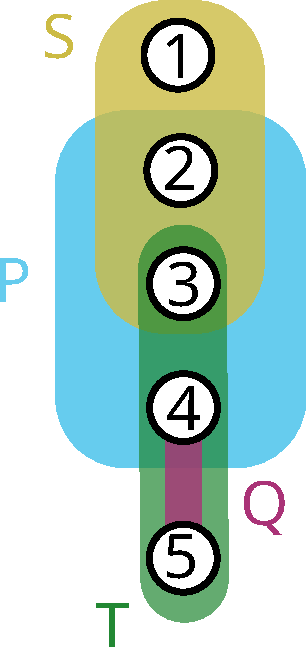
\includegraphics[scale=0.5]{res/example-struct-1}
    \end{minipage}
    \hspace{4em}
    \begin{minipage}[t]{0.6\textwidth}
      {%
      \newcommand{\tups}{{\color{tolbrightYellowDarker}\elemtuples}}%
      \newcommand{\tupp}{{\color{tolbrightCyanDarker}\elemtuplep}}%
      \newcommand{\tupt}{{\color{tolbrightGreen}\elemtuplet}}%
      \newcommand{\tupq}{{\color{tolbrightPurple}\elemtupleq}}%
      The picture on the left shows a structure with the relations: $(1,2,3) \in \relS^{\str{A}}$, $(2,3,4) \in \relP^{\str{A}}$, $(3,4,5) \in \relT^{\str{A}}$, $(4,5) \in \relQ^{\str{A}}$.

      \vspace{1ex}
      Let $\tups = (1, 2, 3), \tupp = (2, 3, 4), \tupt = (3, 4, 5), \tupq = (4,5)$.

      \vspace{1ex}
      Some examples of biseqs in this structure are:
      \begin{itemize}
          \item $\tups(3,3)\tupt$,
          \item $\tups(2,3)\tupp(2,3)\tupt$.
      \end{itemize}

      Biseqs are not required to use maximal infixes, so the following are also valid biseqs:
      \begin{itemize}
          \item $\tups(2,2)\tupp$,
          \item $\tups(3,3)\tupt(2,2)\tupq$.
      \end{itemize}
      }
    \end{minipage}
    \caption{Examples of biseqs.}%
    \label{fig:biseq-examples}
\end{figure}

Let $\Seq{\str{A}}$ be the set of all biseqs for a structure $\str{A}$.
There is a natural projection $\Pi$ from a biseq $\sigma \in \Seq{A}$ to tuples of $\str{A}$: for $\sigma = \cdots (i,j) \elemtuples$, we define $\Pi(\sigma)$ as $\Pi(\sigma) = \elemtuples$.
Intuitively, this projection gives the tuple of selected elements in structure $\str{A}$ in the bisimulation game after playing the moves of $\sigma$.
We now introduce ``bipoints'', which instead of tuples, project to individual selected elements (``points'') of $\str{A}$.
A \emph{bipoint} of a structure $\str{A}$ is a tuple $(\sigma, k) \in \Seq{A} \times \mathbb{N}$ such that
\begin{itemize}
  \item $\sigma = \elemtuplea$, $k \ge 1$ and $k \le |\elemtuplea|$ for some $\elemtuplea \sqin A$, or
  \item $\sigma = \cdots (i,j) \elemtuplea$, $k \ge (j-i+1) + 1$ and $k \le |\elemtuplea|$ for some $\elemtuplea \sqin A$.
\end{itemize}
For a bipoint $e$ of a structure $A$ that can be decomposed as $e = (\rho, k)$, we use the notation $\seq{e} = \rho$ and $\ctr{e} = k$ to denote the biseq and the counter of this bipoint, respectively.
The counter of the bipoint identifies one component of the tuple of elements that the biseq projects to.
We define the projection $\pi$ from bipoints of a structure $\str{A}$ to elements of $\str{A}$ as: if $e = (\sigma, k)$ is a bipoint, then $\pi(e) = {\Pi(\sigma)}_{k}$ (= $\elema_{k}$ for $\sigma = \cdots\elemtuplea$).
The condition that ``$k \ge (j-i+1) + 1$'' ensures that we do not have more than one bipoint for the shared elements in a move in the bisimulation game.
\cref{ex:bipoints} shows a concrete application for this condition.

\begin{example}\label{ex:bipoints}
   {%
     \newcommand{\tups}{{\color{tolbrightYellowDarker}\elemtuples}}%
     \newcommand{\tupt}{{\color{tolbrightGreen}\elemtuplet}}%
     \newcommand{\es}{{\color{tolbrightYellowDarker}s}}%
     \newcommand{\et}{{\color{tolbrightGreen}t}}%
     Consider the biseqs from \cref{fig:biseq-examples}.
     The bipoints for the 0-biseq $\sigma$ with $\sigma = \tups$ are: $a = (\sigma, 1)$, $b = (\sigma, 2)$ and $c = (\sigma, 3)$.
     These project to the components of the tuple $\tups$: $\pi(a) = \es_{1} = 1$, $\pi(b) = \es_{2} = 2$ and $\pi(c) = \es_{3} = 3$.
     Now consider the 1-biseq $\rho$ with $\rho = \tups(3,3)\tupt$.
     Regarded in terms of the game, this sequence represents the move from $\tups$ to $\tupt$, sharing the element ``3''.
     There are bipoints $d = (\rho, 2)$ and $e = (\rho, 3)$ which project to the domain elements ``4'' and ``5''.
     However, there is no bipoint for the sequence $\rho$ that projects to ``3''.
     While $(\rho, 1)$ projects to ``3'' according to the definition of $\pi$, it is not a bipoint as it violates the ``$k \ge (j-i+1) + 1$'' condition in the above definition.
     Note that $c = (\sigma, 3)$ projects to ``3'', so there already is a bipoint that projects to ``3'', using the sequence $\sigma$.
     In fact, bipoints correspond one-to-one to unshared elements of moves in the bisimulation game.
     From the point of view of the biseq $\sigma$, the element ``3'' is not shared with previously selected elements (there are none, since $\sigma$ represents the start of the game at tuple $\tups$), while relative to the biseq $\rho$, the element ``3'' is among the shared elements.
     Hence, $(\sigma, 3)$ is a bipoint, while $(\rho ,1)$ is not.
   }
\end{example}

%!TEX root = ../main.tex
\chapter{Expressive Completeness}\label{chap:expressivity}
Expressive completeness of a fragment $\logicL$ of $\FO$ means that this fragment is complete with respect to some class of properties, \ie{} that for any property of this class, there is a formula in $\logicL$ that expresses this property.
Here, we focus on the special class of properties expressible as \emph{bisimulation-invariant} first-order formulae, which are formulae that do not distinguish between bisimilar structures.
More precisely, a first-order formula $\varphi$ is $\bisimto_{\logicL}$-invariant for a given notion of bisimulation $\bisimto_{\logicL}$ if whenever $\str{A}, \elemtuplea \bisimto_{\logicL} \str{B}, \elemtupleb$, then $\str{A}, \elemtuplea \models \varphi \Leftrightarrow \str{B}, \elemtupleb \models \varphi$.
Similarly, a formula $\varphi$ of $\FO$ is \emph{$\bisimto_{\logicL}$-invariant in the finite} if it does not distinguish between bisimilar structures which are finite (it may however distinguish between \emph{infinite} bisimilar structures, which makes this different from the general, infinite case).
We say that $\logicL$ is \emph{expressively complete} (in the finite) with respect to $\bisimto_{\logicL}$-invariant first-order properties if every $\bisimto_{\logicL}$-invariant formula is equivalent (in the finite) to some formula of $\logicL$.
In this chapter, we show that $\FGF$ is expressively complete with respect to $\bisimto_{\FGF}$-invariant first-order properties, both in the classical sense and in the finite.
We first present a short review of related preservation theorems in \cref{sec:related-work} and then prove a van Benthem theorem for $\FGF$.
We give the high-level structure of the proof, leaving concrete details to be filled in by later chapters.

We already saw in the previous chapter (in \cref{lem:FGF-bisimulations-work-well}) that every $\FGF$ formula is invariant under $\FGF$-bisimulation.
Combined with the result of this chapter, this means that the properties expressible as $\FGF$-formula are precisely those first-order properties that are $\bisimto_{\FGF}$-invariant.
In general, we say that a logic $\logicL$ is the \emph{$\bisimto_{\logicL}$-invariant fragment} of $\FO$ (in the finite) if all formulae of $\logicL$ are $\bisimto_{\logicL}$-invariant and every $\bisimto_{\logicL}$-invariant first-order formula is equivalent (in the finite) to some formula of $\logicL$.
This allows us to formulate the central theorem of this thesis, which we prove at the end of this chapter.
\begin{restatable*}{maintheorem}{vanbenthemFGF}\label{thm:main}
The forward guarded fragment is the $\bisimto_{\FGF}$-invariant fragment of $\FO$, both in the sense of classical model theory and in the finite.
\end{restatable*}

\section{Related Work}\label{sec:related-work}
We focus on \emph{preservation theorems}, which characterize a logic $\logicL$ as a fragment of a richer logic $\logicL'$ as exactly the fragment that is able to express all properties preserved under some form of structural equivalence.
Other ways of measuring the expressive power of logics, such as Lindström theorems~\cite{lindstrom1969, benthem2009} which characterize $\logicL$ as being the maximally expressive logic that still has certain model-theoretic properties are out of scope for this work.

There is a large body of work extending van Benthem's classical result for basic modal logic~\cite{van1983modal} to other variants of modal logic.
Examples of this include:
\begin{itemize}
  \item Rosen's result shows that van Benthem's theorem also works in the finite~\cite{Rosen97}.
  \item Modal logics with multiple, global and inverse modalities are bisimulation invariant fragments of $\FO$ for notions of bisimulation, over both finite and infinite structures~\cite{Otto04}.
  \item Graded modal logic characterized as the counting bisimulation invariant fragment of $\FO$, over both finite and infinite relational structures \cite{derijke2000,otto2023}.
  \item $\GF$ is the $\GF$-bisimulation invariant fragment of $\FO$, both in the classical~\cite{AndrekaNB98} and finite setting~\cite{Otto2012}.
  \item Modal logic extended with fixed point operators ($\mu\ML$) is the bisimulation-invariant fragment of monadic second-order logic ($\Logic{MSO}$) (Janin-Walukiwicz theorem)~\cite{janin1996}, and similar for the guarded fragment extended with fixed point operators~\cite{gradel2002}.
        However, whether this is true in the finite as well is a long-standing open question.
  \item First-order logic restricted to two variables ($\FO{}2$) is the two-pebble game invariant fragment of $\FO$~\cite{gradel1999}, but not in the finite~\cite{otto2017}.
        This shows that the notion of being $\bisimto_{\logicL}$-invariant and being $\bisimto_{\logicL}$-invariant in the finite do not coincide.
  \item Sabotage modal logic, which extends modal logic with an ``edge-deletion'' operator, is the sabotage-bisimulation invariant fragment of $\FO$~\cite{aucher2015}.
  \item Coalgebaric modal logic is, under some constraints, the behavioral-equivalence invariant fragment of Coalgebaric Predicate Logic~\cite{litak2012}, both in the finite and the classical sense.
  \item Concept expressions of different description logics including \Logic{FL^{-}}, \Logic{FLU^-}, \Logic{ALC}, \Logic{ALCQIO}, \Logic{DL{-}Lite} and others are fragments of $\FO$ invariant under corresponding equivalence relations~\cite{kurtonina1999, lutz2011, piro2013}.
  \item $\Logic{XPath}_{=}$, a logic able to express (parts of) the navigational aspect of the XPath XML query language, is a $\FO$ fragment invariant under a corresponding notion of bisimulation for different navigational axes (child, descendant)~\cite{figueira2015}.
  \item \Logic{HornALC} is the Horn-simulation invariant fragment of $\FO$~\cite{jung2019}.
  \item Weakly Aggregative Modal Logic, a polyadic modal logic, is the $wa$-bisimulation invariant fragment of $\FO$~\cite{liu2019}.
\end{itemize}
With the exception of the guarded fragments and the last example, all these results are for logics where predicates have an arity of at most two or allow for at most two variables.
Van Benthem characterizations of logics that allow higher-arity predicates or more than two variables are rarely found.
Two notable examples are the unary negation fragment ($\Logic{UNFO}$)~\cite{segoufin2013} together with its extension, the guarded negation fragment ($\Logic{GNFO}$)~\cite{barany2015}, and the forward fragment ($\Logic{FF}$)~\cite{BednarczykJ22}, which all have a van Benthem characterization in terms of a corresponding notion of bisimulation.
In the case of $\Logic{UNFO}$, this characterization works also in the finite, while in the case of $\Logic{GNFO}$, a finite version is only known for a restricted version limited to $k$ variables.
In the case of the forward fragment, a characterization in the finite is an open problem.

A possible reason for the popularity of logics without higher-arity relations may be that higher-arity relations are difficult to work with, as demonstrated by the proof of the van Benthem characterization of $\GF$~\cite{Otto2012}.
Compared to an earlier result for $\GF$ with relations of arity at most 2~\cite{Otto04}, the details of this proof are much more complex.
Luckily, since $\FGF$ is a subset of $\GF$ and any formula preserved under $\FGF$-bisimulation is also preserved under $\GF$-bisimulation, we can focus on characterizing $\FGF$ as a subset of $\GF$ here.
The full van Benthem theorem for $\FGF$ then follows from Otto's van Benthem theorem for $\GF$.

The proof technique in this thesis closely follows the approach taken by Otto to prove van Benthem theorems for variations of modal logic~\cite{Otto04, otto2004a}.
The central part of this technique is the construction of structures called ``finite companions''.
Like Otto, we construct these companions by stopping the infinite unraveling at some depth and then relinking edges to roots, to preserve similarity with the original structure.
The method of unraveling that we employ is inspired by the construction that Bednarczyk used to show the $\ExpTime$-completeness of $\FGF$~\cite{Bednarczyk21}.
Bednarczyk's construction however is not sufficient to construct the finite companions.
Our new method turns out to be similar to a method of unraveling already described by Andréka et al. when introducing the guarded fragment~\cite{AndrekaNB98}.
We present a comparison to these two existing methods of unraveling in \cref{sec:existing-unravelings}.
In the next section, we introduce our approach to prove van Benthem for $\FGF$ following Otto in detail.

\section{Van Benthem for $\FGF$}\label{sec:van-benthem-theorem}
The high-level idea for the proof of the van Benthem theorem for $\FGF$ is to show that for any given $\bisimto_{\FGF}$ first-order formula $\varphi$, there is some number $\ell \in \N$ such that $\varphi$ is $\bisimto_{\FGF}^{\ell}$ invariant.
An observation by Otto~\cite[Obs.~13]{Otto04} then implies the above theorem.
In the following, we present this observation in full for $\FGF$.
First, we can see that every $\bisimto_{\FGF}^{\ell}$ equivalence class is characterized by an $\FGF_{\ell}$ formula, as stated in the following lemma:
\begin{lemma}
  For any structure $(\str{A}, \elemtuplea)$ and $\ell \in \N$, there is a formula $\chi_{(\str{A}, \elemtuplea)} \in \FGF_{\ell}$ such that $(\str{A}, \elemtuplea) \models \chi_{(\str{A}, \elemtuplea)}$, but $(\str{B}, \elemtupleb) \not\models \chi_{\str{A}, \elemtuplea}$ for every structure $(\str{B}, \elemtupleb) \nsim^{\ell}_{\FGF} (\str{A}, \elemtuplea)$.
\end{lemma}
\begin{proof}
  Let $\Gamma$  be the set of all $\FGF_{\ell}$ formulae which are satisfied in $(\str{A}, \elemtuplea)$, so
  \begin{equation*}
    \Gamma = \{ \psi:\, \psi \in \FGF_{\ell} \text{ and } (\str{A}, \elemtuplea) \models \psi \}.
  \end{equation*}
  Since the number of logically inequivalent $\FGF_{\ell}$ formula is finite, there is a set $\Delta$ that is finite and logically equivalent to $\Gamma$.
  We show that $\chi_{(\str{A}, \elemtuplea)} = \bigwedge \Delta$ satisfies the above lemma.
  For any structure $(\str{B}, \elemtupleb)$ with $(\str{B}, \elemtupleb) \nsim_{\FGF}^{\ell} (\str{A}, \elemtuplea)$, by \cref{lem:FGF-bisimulations-work-well} there is a formula $\varphi$ in $\FGF_{\ell}$ such that $(\str{A}, \elemtuplea) \models \varphi$ but $(\str{B}, \elemtupleb) \not\models \varphi$.
  But $(\str{A}, \elemtuplea) \models \varphi$ means that $\varphi \in \Gamma$ and hence $\chi_{(\str{A},\elemtuplea)} \to \varphi$.
  Since $(\str{B}, \elemtupleb) \not\models \varphi$, we have $(\str{B}, \elemtupleb) \not\models \chi_{(\str{A}, \elemtuplea)}$ as required.
\end{proof}
Because the characteristic formula $\chi_{(\str{A}, \elemtuplea)}$ is an $\FGF_{\ell}$ formula, there are only a finite number of logically inequivalent characteristic formulae.
It follows that $\bisimto_{\FGF}^{\ell}$ has a finite number of equivalence classes.
For a $\bisimto_{\FGF}^{\ell}$-invariant formula $\varphi$, we can hence enumerate all equivalence classes of $\bisimto_{\FGF}^{\ell}$ in which $\varphi$ is satisfied, and take the disjunction of their characteristic formulae to obtain an equivalent $\FGF_{\ell}$ formula.
This leads to the following corollary:
\begin{corollary}\label{cor:ell-invariant-has-ell-formula}
  For any $\ell \in \N$, every $\bisimto_{\FGF}^{\ell}$-invariant $\FO$ formula $\varphi$ is equivalent to some formula in $\FGF_{\ell}$.
\end{corollary}

\noindent
Our proof for the van Benthem characterization of $\FGF$ relies on the van Benthem characterization of $\GF$ provided by Otto~\cite{Otto2012}.
For convenience, we restate this result here, in the form of the following theorem.
\begin{theorem}[Theorem 4.7 by Otto~\cite{Otto2012}]\label{thm:vanBenthem-for-GF}
  The guarded fragment is the $\bisimto_{\GF}$-invariant fragment of $\FO$, both in the sense of classical model theory and in the finite.
  More specifically, there is a computable function $\homof \colon \N \to \N$ such that every $\FO$-formula $\varphi$ of quantifier rank $q$ that is $\bisimto_{\GF}$-invariant (in the finite) is also $\bisimto^{\homof(q)}_{\GF}$-invariant (in the finite) and logically equivalent (in the finite) to a $\GF$-formula of quantifier rank at most $\homof(q)$.
\end{theorem}
Additionally, we state the following theorem, which is the main technical theorem whose proof we develop through \cref{chap:unraveling} and \cref{chap:finite}.
\begin{restatable*}{theorem}{maintechnicalthm}\label{thm:main-technical-thm}
  There exists a positive polynomial function~$\homop$ such that for every $\ell$ and every pair of $\homop(\ell)$-$\FGF$-bisimilar pointed structures, there exists $\FGF$-bisimilar companions $(\str{A}', \elemtuplea')$ and $(\str{B}', \elemtupleb')$ (that are finite if $\str{A}$ and $\str{B}$ are) of $(\str{A}, \elemtuplea)$ and $(\str{B}, \elemtupleb)$ such that $(\str{A}', \elemtuplea') \bisimto^{\ell}_{\GF} (\str{B}', \elemtupleb')$.
\end{restatable*}

\noindent
Note that the companions from \cref{thm:main-technical-thm} are not only $\ell$-$\FGF$-bisimilar, but even $\ell$-$\GF$ bisimilar. Finally, we show how these two theorems combined imply our main theorem, the van Benthem characterization of $\FGF$.
\ifmainpart
\vanbenthemFGF
\else
  \section{Main Theorem}
  \vanbenthemFGF*
\fi
\ifmainpart
\newsavebox{\diagupgrading}
\begin{lrbox}{\diagupgrading}{
  \begin{tikzpicture}
    \matrix[row sep=2em, column sep=3em]
    {
        \node (a) {$(\str{A}, \elemtuplea)$}; &
         \node[font=\large] (sim_ab) {$\bisimto_{\FGF}^{\homop(\mathit{g})}$}; &
        \node (b) {$(\str{B}, \elemtupleb)$}; &
        \node[anchor=west] {}; \\

        \node[font=\large] (sim_a_unravel) {$\bisimto_{\FGF}$}; &
        \node {}; &
        \node[font=\large] (sim_b_unravel) {$\bisimto_{\FGF}$}; &
        \node[anchor=west] {}; \\

        \node (a_unravel) {$(\str{A}', \elemtuplea')$}; &
        \node[font=\large] (sim_unravel) {$\bisimto_{\GF}^{\mathit{g}}$}; &
        \node (b_unravel) {$(\str{B}', \elemtupleb')$};
        \node[anchor=west] {}; \\
    };

    \draw[->] (a) -- (sim_ab) -> (b);
    \draw[dashed,->] (a) -- (sim_a_unravel) -> (a_unravel);
    \draw[->] (a_unravel) -- (sim_unravel) -> (b_unravel);
    \draw[dashed,->] (b_unravel) -- (sim_b_unravel) -> (b);
  \end{tikzpicture}
}
\end{lrbox}
\begin{proofsketch}
  The invariance of $\FGF$ under $\bisimto_{\FGF}$ was already shown in \cref{lem:FGF-bisimulations-work-well}, hence what is left to show is the expressive completeness.
  By \cref{cor:ell-invariant-has-ell-formula}, it suffices to show that for every first-order formula that is $\bisimto_{\FGF}$-invariant (in the finite) is also $\bisimto_{\FGF}^{\ell}$-invariant (in the finite) for some $\ell \in \N$.
  Like Otto, we employ an``upgrading'' to show this.
  For structures $\str{A}, \elemtuplea$ and $\str{B}, \elemtupleb$, the upgrading is shown in the following diagram:
  \begin{center}%
    \usebox{\diagupgrading}
  \end{center}
  where $\str{A'}, \elemtuplea'$, $\str{B'}, \elemtupleb'$ are the companions and $\homop$ is the polynomial function as given by \cref{thm:main-technical-thm}.
  For every $\bisimto_{\FGF}$-invariant (and hence also $\bisimto_{\GF}$-invariant) $\FO$-formula $\phi$, there is a $g$ such that $\phi$ is $\bisimto_{\GF}^{g}$ invariant (\cref{thm:vanBenthem-for-GF}).
  By the above diagram, this implies that $\phi$ is $\bisimto_{\FGF}^{\homop(g)}$ invariant.
  Since all the structures involved in the proof are finite if $\str{A}, \elemtuplea$ and $\str{B},  \elemtupleb$ are finite, this works for both classical model theory and in the finite, concluding the proof.
\end{proofsketch}
\else
\begin{proof}
  The invariance of $\FGF$ under $\bisimto_{\FGF}$ was already shown in \cref{lem:FGF-bisimulations-work-well}, hence what is left to show is the expressive completeness.
By \cref{cor:ell-invariant-has-ell-formula}, it suffices to show that for every first-order formula that is $\bisimto_{\FGF}$-invariant (in the finite) is also $\bisimto_{\FGF}^{\ell}$-invariant (in the finite) for some $\ell \in \N$.

Take any such first-order formula $\varphi$, and let $\homop$ be the function provided by~\cref{thm:main-technical-thm}.
As $\FGF$ is a fragment of $\GF$ (and hence $\bisimto_{\FGF}$-invariance implies $\bisimto_{\GF}$-invariance), we know that $\varphi$ is $\bisimto_{\GF}$-invariant (in the finite).
Thus $\varphi$ is also $\bisimto_{\GF}^{\mathit{g}}$-invariant (in the finite) for certain threshold $\mathit{g} \in \N$ provided by~\cref{thm:vanBenthem-for-GF}.
We aim to show that $\varphi$ is $\bisimto_{\FGF}^{\homop(\mathit{g})}$-invariant (in the finite).
To do so, let $(\str{A}, \elemtuplea)$ and $(\str{B}, \elemtupleb)$ be $\homop(\mathit{g})$-$\FGF$-bisimilar pointed structures, and suppose that $(\str{A}, \elemtuplea) \models \varphi$. It remains to show that $(\str{B}, \elemtupleb) \models \varphi$.
From~\cref{thm:main-technical-thm} we infer the existence of $\FGF$-bisimilar companions $(\str{A}', \elemtuplea')$ and $(\str{B}', \elemtupleb')$, that are finite if $\str{A}$ and $\str{B}$ are, for which $(\str{A}', \elemtuplea') \bisimto^{\mathit{g}}_{\GF} (\str{B}', \elemtupleb')$ holds.
The following diagram depicts what will happen next.
\begin{figure}[H]
  \centering
  \usebox{\diagupgrading}
  % \caption{Upgrading $\bisimto_{\FGF}^{\ell}$-bisimulation to $\bisimto_{\GF}^{\mathit{g}}$-bisimulation.}
\end{figure}

It is now clear that:
(i) $(\str{A}, \elemtuplea) \models \varphi$ (by assumption),
(ii) $(\str{A}', \elemtuplea') \models \varphi$ (by $\FGF$-bisimilarity and $\bisimto_{\FGF}$-invariance of $\varphi$),
(iii) $(\str{B}', \elemtupleb') \models \varphi$ (by $\bisimto_{\GF}^{\mathit{g}}$-invariance of $\varphi$),
(iv) $(\str{B}, \elemtupleb) \models \varphi$ (by $\FGF$-bisimilarity and $\bisimto_{\FGF}$-invariance of $\varphi$).
This concludes the proof.
\end{proof}
\fi


%!TEX root = ../main.tex
\chapter{Tree Unravelings}\label{chap:unraveling}
A fundamental property of modal logics is that their models are tree-like, which roughly speaking means they look like trees as known from graph theory (we give an exact definition later).
We show in this chapter that a special form of tree models can be characterized unusually well by $\FGF$ formulae (they provide logically tractable models for $\FGF$, in the sense of~\cite{otto2013}).
In this class of models, the weak form of $\bisimto_{\FGF}$-equivalence coincides with the stronger notion of $\bisimto_{\GF}$-equivalence.
To obtain such models, we introduce a new notion of tree unraveling for $\FGF$, which takes an arbitrary model and constructs a structure which is bisimilar to this model but additionally is tree-like.
An explanation for why we need a new unraveling is provided in the first section of this chapter, where we give a short review of existing notions of unraveling for $\FGF$ and $\GF$.
In essence, the tree model obtained via our new method of unraveling provides a representative for a $\bisimto_{\FGF}$ equivalence class, which is unique up to $\bisimto_{\GF}$-equivalence.
This is the first step towards the construction of finite companions as required for \cref{thm:main-technical-thm}.
The following theorem highlights the main property of our new notion of unraveling for $\FGF$, developed in this chapter:
\begin{restatable*}{theorem}{thminfupgrading}\label{thm:inf-bisim-upgrading}
  For unravelings $(\unravel{A}, \elemtuptuplea)$ and $(\unravel{B}, \elemtuptupleb)$  of two structures $(\str{A}, \elemtuplea)$ and $(\str{B}, \elemtupleb)$, if $(\unravel{A}, \elemtuptuplea) \bisimto_{\FGF} (\unravel{B}, \elemtuptupleb)$ then $(\unravel{A}, \elemtuptuplea) \bisimto_{\GF} (\unravel{B}, \elemtuptupleb)$.
\end{restatable*}%

For structures $\str{A}$ with a distinguished binary predicate $\relNext$, we employ tailored terminology from graph theory.
For instance, whenever $(\eleme_1, \eleme_2) \in \relNext^{\str{A}}$, we call the element $\eleme_2$ a \emph{child} of $\eleme_1$. Respectively, we call $\eleme_1$ a \emph{parent} of $\eleme_2$.
A \emph{root} is an element without parents.
The set of \emph{descendants} of an element $\eleme$ is the smallest set containing $\eleme$ that is closed under taking children (\ie{} if an element is in the set then so are its children).
We call a structure $\str{A}$ a \emph{forest} if every element has at most one parent and is a descendant of some root.
A forest is a \emph{tree} if it has exactly one root.
We say that a model is a \emph{forest model} (or \emph{tree model}) if its restriction to $\relNext$ is a forest (or tree).

\section{Existing notions of unraveling for $\FGF$ and $\GF$}\label{sec:existing-unravelings}
In this section, we review two existing notions of tree unraveling, one for $\FGF$ and one for $\GF$.
This is helpful to understand the motivation for our new unraveling.
Readers who are only interested in the new unraveling may safely skip this section.

We focus on structures $\str{A}$ without distinguished elements here, to simplify the definitions.
However, extending these definitions to pointed structures $(\str{A}, \elemtuplea)$ is not difficult.
We start with the definitions, and show some examples afterwards.
We begin with the unraveling for $\GF$, as described by Andréka et al.~\cite[Sec 4.3, p. 247]{AndrekaNB98}.
\begin{definition}[$\GF$-unraveling]
  The domain of the \emph{$\GF$-unraveling} $\gfunravel{A}$ of a structure $\str{A}$ consists of pairs $(\rho, a)$ where $\rho$ is a finite sequence of guarded sets and $a \in A$ is an element which is ``new'' in $\rho$: it occurs in the last set of $\rho$, but not in the one before that.
  Every relation $\relR \in \Sigma$ is interpreted in $\gfunravel{A}$ as follows: for a tuple $\gfunraveltup{a} = ((\rho_{1}, a_{1}), \ldots, (\rho_{n}, a_{n}))$ with $n \in \N$, we let $\gfunraveltup{a} \in \relR^{\gfunravel{A}}$ if:
  \begin{enumerate}
    \item $(a_{1}, \ldots, a_{n}) \in \relR^{\str{A}}$, \ie{} the ``new'' elements of each pair are related by $\relR$ in the base structure,
    \item there is a maximal sequence $p_{j}$: for some $j \in [1,n]$, every $\rho_{i}$ for $i \in [1,n]$ is a prefix of $\rho_{j}$,
    \item the new elements $a_{i}$ remain present in each guarded set from $\rho_{i}$ to the end of $\rho_{j}$.
  \end{enumerate}
\end{definition}
As expected, the $\GF$-unraveling $\gfunravel{A}$ is $\GF$-bisimilar to the original structure $\str{A}$~\cite[Proposition 4.3.1]{AndrekaNB98}.

For comparison, we now present the \emph{HAF-unraveling}, an unraveling for $\FGF$ introduced by Bednarczyk~\cite[Sec 3.3]{Bednarczyk21}.
Our presentation here is based on a later version of this unraveling, the \emph{HAH-unraveling}~\cite[Appendix C.4, Definition 20]{BednarczykJ22}, which is the same as the HAF-unraveling for signatures without constants.
\begin{definition}[HAH-unraveling]
  The domain of the \emph{HAH-unraveling} $\hatunravel{A}$ of a structure $\str{A}$ contains all finite sequences $\rho = a_{1}\cdots{}a_{n}$ of elements from $A$ for all $n \in \N^{+}$, with the following additional property:
  For every $i \in [1,n-1]$, the elements $a_{i}, a_{i+1}$ appear consecutively in some relation, \ie{} there are tuples $\elemtuplee, \elemtuplef \sqin A$  of elements from $\str{A}$ such that, for some relation $\relR \in \Sigma$:
  \begin{equation*}
    \elemtuplee{}\,a_{i}\,a_{i+1}\,\elemtuplef{} \in \relR^{\str{A}}.
  \end{equation*}
  For each sequence $\rho$ in the domain, we define $\mathrm{last}(\rho) = a$ where $a$ is the last element of $\rho$, \ie{} $\rho = \cdots a$.
  Every relation $\relR \in \Sigma$ is interpreted in $\hatunravel{A}$ as follows: for a tuple $\hatunraveltup{a} = (\rho_{1}, \ldots, \rho_{n})$ with $n \in \N$, we let $\hatunraveltup{a} \in \relR^{\hatunravel{A}}$ if:
  \begin{enumerate}
    \item $(\mathrm{last}(\rho_{1}), \ldots, \mathrm{last}(\rho_{n})) \in \relR^{\str{A}}$, \ie{} the last elements of each sequence are related by $\relR$ in the base structure, and
    \item there are elements $e_{2}, \ldots, e_{n} \in A$ such that $\rho_{i} = \rho_{1}e_{1}\cdots{}e_{i}$ for all $i \in [2,n]$.
  \end{enumerate}
\end{definition}
Similarly to the case for $\GF$, the HAH-unraveling $\hatunravel{A}$ is $\FGF$-bisimilar to the original structure $\str{A}$~\cite[Appendix C.4, Lemma 23]{BednarczykJ22}.

\begin{example}
  \newlength\figindent\setlength\figindent{7em}%
  \newlength\figdist\setlength\figdist{2em}%
  To demonstrate the above definitions, consider the following structure $\str{A}$:\\[1ex]
  \begin{minipage}{\figindent}
    \raggedleft
    \vphantom{$A = \{1,2,3,4\}$}\\[0.7ex]
    {\Huge{$\str{A}$}}\\[0.5ex]
    {$A = \{1,2,3,4\}$}
  \end{minipage}
  \hspace{\figdist}
  \begin{tikzpicture}[baseline]
  \tikzset{el/.style={circle,draw,fill=white,minimum width=2em,minimum height=2em}};
  \tikzset{relP/.style={tolhighcontrastBlue, line width=0.4em, -{Stealth[round]}, shorten >= 0.4em}};
  \tikzset{relE/.style={tolhighcontrastYellow, line width=0.25em, -{Stealth[round]}, shorten >= 0.2em}};
  \tikzset{relS/.style={tolhighcontrastRed, line width=0.15em, -{Stealth[round]}, shorten >= 0.2em}};
  \def\radiusP{0.7em};
  \def\radiusE{0.4em};
  \def\radiusS{0.2em};

  \matrix[matrix of nodes, every node/.style={el}, column sep=4em] {
    |(n1)| 1 & |(n2)| 2 & |(n3)| 3 & |(n4)| 4  \\
  };

  \begin{scope}[on background layer]
    % 1 2 3
    \fill[relP] (n1.north) circle[radius=\radiusP] coordinate (p1);
    \fill[relP] (n2.north) circle[radius=\radiusP] coordinate (p2);
    \fill[relP] (n3.north west) circle[radius=\radiusP] coordinate (p3);
    \draw[relP] (p1) to[out=30,in=150] (p2) to[out=30,in=150] (p3);

    % 4 3 2
    \fill[relP] (n4.south) circle[radius=\radiusP] coordinate (p1);
    \fill[relP] (n3.south) circle[radius=\radiusP] coordinate (p2);
    \fill[relP] (n2.south) circle[radius=\radiusP] coordinate (p3);
    \draw[relP] (p1) to[in=-30,out=-150] (p2) to[in=-30,out=-150] (p3);

    % 3 4
    \fill[relE] ($(n3.east) + (0,-0.2em)$) circle[radius=\radiusE] coordinate (p1);
    \fill[relE] (n4.west) circle[radius=\radiusE] coordinate (p2);
    \draw[relE] (p1) to (p2);

    % 1 3
    \fill[relE] (n1.west) circle[radius=\radiusE] coordinate (p1);
    \fill[relE] (n3.north east) circle[radius=\radiusE] coordinate (p2);
    \draw[relE] (p1) to[out=140,in=north] (p2);

    % 1 2
    \fill[relS] (n1.east) circle[radius=\radiusS] coordinate (p1);
    \fill[relS] (n2.west) circle[radius=\radiusS] coordinate (p2);
    \draw[relS] (p1) to[out=east,in=west] (p2);

    \fill[relS] (n2.east) circle[radius=\radiusS] coordinate (p1);
    \fill[relS] ($(n3.west) + (0,-0.2em)$) circle[radius=\radiusS] coordinate (p2);
    \draw[relS] (p1) to[out=east,in=west] (p2);
  \end{scope}

  \begin{scope}[on background layer]
    %\tikzdbg
  \end{scope}
\end{tikzpicture}
\\

  \noindent
  We first draw unravelings and explain some details.
  For the $\GF$-unraveling, the guarded sets of $\str{A}$ are:
  \begin{equation*}
    s_{1} = \{1,2\}\quad
    s_{2} = \{1,3\}\quad
    s_{3} = \{1,2,3\}\quad
    s_{4} = \{2,3,4\}\quad
    s_{5} = \{2,3\}\quad
    s_{6} = \{3,4\}\quad
  \end{equation*}
  Since we can form elements of the $\GF$-unraveling from any finite sequence of those sets, the $\GF$-unraveling is infinite.
  The following figure shows a substructure of the full unraveling.
  For better readability, we use $\rho / a$ to denote the pair $(\rho, a)$ for a sequence $\rho$ and an element $a \in A$.\\[2ex]
  \begin{minipage}{\figindent}
    \raggedleft
    part of \Huge{$\gfunravel{A}$}
  \end{minipage}
  \hspace{\figdist}
  \begin{tikzpicture}
  \tikzset{el/.style={rectangle,rounded corners=10pt,draw,fill=white,minimum width=2em,minimum height=2em,font=\small}};
  \tikzset{relP/.style={tolhighcontrastBlue, line width=0.4em, -{Stealth[round]}, shorten >= 0.4em}};
  \tikzset{relE/.style={tolhighcontrastYellow, line width=0.25em, -{Stealth[round]}, shorten >= 0.2em}};
  \tikzset{relS/.style={tolhighcontrastRed, line width=0.15em, -{Stealth[round]}, shorten >= 0.2em}};
  \def\radiusP{0.7em};
  \def\radiusE{0.4em};
  \def\radiusS{0.2em};

  \matrix[matrix of nodes, every node/.style={el}, column sep=2em, row sep=2em] {
    |(s1s23)| $s_{1}s_{2} / 3$ & |(s1s5s31)| $s_{1}s_{5}s_{3} / 1$ & & |(s1s44)| $s_{1}s_{4}/4$ \\
    |(s11)| $s_{1} / 1$ & |(s12)| $s_{1} / 2$ & |(s1s53)| $s_{1}s_{5} / 3$ & |(s1s43)| $s_{1}s_{4}/3$   \\
    & |(s1s33)| $s_{1}s_{3} / 3$ & &  \\
  };

  \begin{scope}[on background layer]
    \fill[relS] (s11.east) circle[radius=\radiusS] coordinate (p1);
    \fill[relS] (s12.west) circle[radius=\radiusS] coordinate (p2);
    \draw[relS] (p1) to[out=east,in=west] (p2);

    \fill[relS] ($(s12.east)+(-0.1em,0.4em)$) circle[radius=\radiusS] coordinate (p1);
    \fill[relS] (s1s53.west) circle[radius=\radiusS] coordinate (p2);
    \draw[relS] (p1) to[out=-20,in=west] (p2);

    \fill[relS] ($(s12.east)+(0em,-0.1em)$) circle[radius=\radiusS] coordinate (p1);
    \fill[relS] ($(s1s43.south)+(-1em,0em)$) circle[radius=\radiusS] coordinate (p2);
    \draw[relS] (p1) to[out=-30,in=south west] (p2);

    \fill[relS] ($(s1s5s31.south)+(-1em,0em)$) circle[radius=\radiusS] coordinate (p1);
    \fill[relS] ($(s12.west)+(0.1em,0.4em)$) circle[radius=\radiusS] coordinate (p2);
    \draw[relS] (p1) to[out=south west,in=north west] (p2);

    \fill[relS] (s12.south) circle[radius=\radiusS] coordinate (p1);
    \fill[relS] (s1s33.north) circle[radius=\radiusS] coordinate (p2);
    \draw[relS] (p1) to[out=south,in=north] (p2);

    \fill[relP] (s11.south) circle[radius=\radiusP] coordinate (p1);
    \fill[relP] (s12.south west) circle[radius=\radiusP] coordinate (p2);
    \fill[relP] (s1s33.west) circle[radius=\radiusP] coordinate (p3);
    \draw[relP] (p1) to (p2) to (p3);

    \fill[relP] (s1s5s31.south) circle[radius=\radiusP] coordinate (p1);
    \fill[relP] (s12.north) circle[radius=\radiusP] coordinate (p2);
    \fill[relP] (s1s53.north west) circle[radius=\radiusP] coordinate (p3);
    \draw[relP] (p1) to (p2) to (p3);

    \fill[relP] (s1s44.east) circle[radius=\radiusP] coordinate (p1);
    \fill[relP] (s1s43.south east) circle[radius=\radiusP] coordinate (p2);
    \fill[relP] (s12.south east) circle[radius=\radiusP] coordinate (p3);
    \draw[relP] (p1) to[out=-60,in=60] (p2) to[out=-150,in=south east] (p3);

    \fill[relE] (s1s43.north) circle[radius=\radiusE] coordinate (p1);
    \fill[relE] (s1s44.south) circle[radius=\radiusE] coordinate (p2);
    \draw[relE] (p1) to (p2);

    \fill[relE] (s1s5s31.east) circle[radius=\radiusE] coordinate (p1);
    \fill[relE] (s1s53.north) circle[radius=\radiusE] coordinate (p2);
    \draw[relE] (p1) to[out=-30,in=120] (p2);

    \fill[relE] (s11.north) circle[radius=\radiusE] coordinate (p1);
    \fill[relE] (s1s23.south) circle[radius=\radiusE] coordinate (p2);
    \draw[relE] (p1) to (p2);

    \fill[relE] (s11.west) circle[radius=\radiusE] coordinate (p1);
    \fill[relE] (s1s33.south) circle[radius=\radiusE] coordinate (p2);
    \draw[relE] (p1) to[out=-120,in=-120] (p2);

  \end{scope}
\end{tikzpicture}
\\[1ex]

  \noindent
  Next, we construct the HAH-unraveling $\hatunravel{A}$. First, let us draw the graph of elements which appear consecutively in relations, which gives the following picture:\\[1ex]
  \begin{minipage}{\figindent}
    \mbox{}
  \end{minipage}
  \hspace{\figdist}
  \begin{tikzpicture}
  \tikzset{adj/.style={densely dashed,thick,draw}};
  \tikzset{el/.style={circle,draw,fill=white,minimum width=2em,minimum height=2em}};

  \matrix[matrix of nodes, every node/.style={el}, column sep=4em] {
    |(n1)| 1 & |(n2)| 2 & |(n3)| 3 & |(n4)| 4 \\
  };

  \graph[use existing nodes, edges=adj] {
    (n1) -> (n2),
    (n1) ->[bend left] (n3),
    (n2) -> (n3),
    (n3) -> (n4),
    (n4) ->[bend left] (n3),
    (n3) ->[bend left] (n2)
  };
\end{tikzpicture}
\\[1ex]
  The elements of the HAH-unraveling correspond to paths in this graph.
  The following picture shows a part of the unraveling, focusing on paths starting from the element $1$:\\[1ex]
  \begin{minipage}{\figindent}
    \raggedleft
    part of \Huge{$\hatunravel{A}$}
  \end{minipage}
  \hspace{\figdist}
  \begin{tikzpicture}
  \tikzset{el/.style={ellipse,draw,fill=white,minimum width=2.5em,minimum height=2em}};
  \tikzset{adj/.style={densely dashed,thick,draw,opacity=0.8}};
  \tikzset{relP/.style={tolhighcontrastBlue, line width=0.4em, -{Stealth[round]}, shorten >= 0.4em}};
  \tikzset{relE/.style={tolhighcontrastYellow, line width=0.25em, -{Stealth[round]}, shorten >= 0.2em}};
  \tikzset{relS/.style={tolhighcontrastRed, line width=0.15em, -{Stealth[round]}, shorten >= 0.2em}};
  \def\radiusP{0.7em};
  \def\radiusE{0.4em};
  \def\radiusS{0.2em};

  \matrix[matrix of nodes, every node/.style={el}, column sep=2em, row sep=1.2em] {
    & |(n2)| 1\textbf{2} & |(n3)| 12\textbf{3} & |(n4)| 123\textbf{4} & |(n5)| 1234\textbf{3} & |(n6)| 12343\textbf{2} & |[draw=none] (n7)| $\cdots{}$ \\
|(n1)| \textbf{1}  & & & & & & \\
    & |(nx3)| 1\textbf{3} & |(nx4)| 13\textbf{4} & |(nx5)| 134\textbf{3} & |(nx6)| 1343\textbf{2} & |(nx7)| 13434\textbf{3} & |[draw=none] (nx8)| $\cdots{}$ \\
  };
  % extra out of grid nodes
  \begin{scope}[every node/.style={el}]
    \node[above right=2em of nx3,xshift=-1em] (nx32) { 13\textbf{2} };
    \node[above right=2em of nx5,xshift=-2em] (nx54) { 1343\textbf{4} };
    \node[above right=2em of n3,xshift=-1em] (n32) { 123\textbf{2} };
    \node[above right=2em of n5,xshift=-1em] (n54) { 12343\textbf{4} };

    \node[right=1em of nx32,draw=none] (ex32) {$\cdots{}$};
    \node[right=1em of nx54,draw=none] (ex54) {$\cdots{}$};
    \node[right=1em of n32,draw=none] (e32) {$\cdots{}$};
    \node[right=1em of n54,draw=none] (e54) {$\cdots{}$};
  \end{scope}

  \begin{scope}[on background layer]
    \graph[use existing nodes, edges=adj] {
      (n1) -> (n2) -> (n3) -> (n4) -> (n5) -> (n6) -> (n7),
      (n1) -> (nx3) -> (nx4) -> (nx5) -> (nx6) -> (nx7) -> (nx8),
      (n3) -> (n32) -> (e32),
      (n5) -> (n54) -> (e54),
      (nx3) -> (nx32) -> (ex32),
      (nx5) -> (nx54) -> (ex54),
    };
  \end{scope}

  \begin{scope}[on background layer]
    % 1 2 3
    \fill[relP] (n1.north) circle[radius=\radiusP] coordinate (p1);
    \fill[relP] (n2.north) circle[radius=\radiusP] coordinate (p2);
    \fill[relP] (n3.west) circle[radius=\radiusP] coordinate (p3);
    \draw[relP] (p1) to[out=30,in=150] (p2) to[out=30,in=150] (p3);

    % 3 4
    \fill[relE] (n3.east) circle[radius=\radiusE] coordinate (p1);
    \fill[relE] (n4.west) circle[radius=\radiusE] coordinate (p2);
    \draw[relE] (p1) to[out=30,in=150] (p2);

    % 4 3 2
    \fill[relP] (n4.south) circle[radius=\radiusP] coordinate (p1);
    \fill[relP] (n5.south) circle[radius=\radiusP] coordinate (p2);
    \fill[relP] (n6.south) circle[radius=\radiusP] coordinate (p3);
    \draw[relP] (p1) to[out=-30,in=-150] (p2) to[out=-30,in=-150] (p3);

    % x3 x4
    \fill[relE] (nx3.east) circle[radius=\radiusE] coordinate (p1);
    \fill[relE] (nx4.west) circle[radius=\radiusE] coordinate (p2);
    \draw[relE] (p1) to[out=30,in=150] (p2);

    % x4 x3 x2
    \fill[relP] (nx4.south) circle[radius=\radiusP] coordinate (p1);
    \fill[relP] (nx5.south) circle[radius=\radiusP] coordinate (p2);
    \fill[relP] (nx6.south) circle[radius=\radiusP] coordinate (p3);
    \draw[relP] (p1) to[out=-30,in=-150] (p2) to[out=-30,in=-150] (p3);

    % 1 x3
    \fill[relE] (n1.south) circle[radius=\radiusE] coordinate (p1);
    \fill[relE] (nx3.west) circle[radius=\radiusE] coordinate (p2);
    \draw[relE] (p1) to[out=south,in=west] (p2);

    % 1 2
    \fill[relS] (n1.east) circle[radius=\radiusS] coordinate (p1);
    \fill[relS] (n2.south) circle[radius=\radiusS] coordinate (p2);
    \draw[relS] (p1) to[out=east,in=south west] (p2);

    \fill[relS] (n2.south east) circle[radius=\radiusS] coordinate (p1);
    \fill[relS] (n3.south) circle[radius=\radiusS] coordinate (p2);
    \draw[relS] (p1) to[out=south east,in=south west] (p2);

    \fill[relS] (nx6.north east) circle[radius=\radiusS] coordinate (p1);
    \fill[relS] (nx7.north west) circle[radius=\radiusS] coordinate (p2);
    \draw[relS] (p1) to[out=north east,in=north west] (p2);

    \fill[relS] (n6.east) circle[radius=\radiusS] coordinate (p1);
    \draw[relS] (p1) to[out=north east,in=north west] (n7);

    % x7 x8
    \fill[relE] (nx7.east) circle[radius=\radiusE] coordinate (p1);
    \draw[relE] (p1) to[out=30,in=120] (nx8.north west);

    \fill[relE] (n5.north) circle[radius=\radiusE] coordinate (p1);
    \fill[relE] (n54.west) circle[radius=\radiusE] coordinate (p2);
    \draw[relE] (p1) to[out=north,in=west] (p2);

    \fill[relE] (nx5.north west) circle[radius=\radiusE] coordinate (p1);
    \fill[relE] (nx54.west) circle[radius=\radiusE] coordinate (p2);
    \draw[relE] (p1) to[out=north,in=west] (p2);

    \fill[relP] (n54.north east) circle[radius=\radiusP] coordinate (p1);
    \draw[relP,tips=never] (p1) to[out=north east] (e54);

    \fill[relP] (nx54.south east) circle[radius=\radiusP] coordinate (p1);
    \draw[relP,tips=never] (p1) to[out=south east, in=south west] (ex54);

  \end{scope}

\end{tikzpicture}
\\[2ex]
  The black, dashed edges show the underlying tree structure of this unraveling.

  Observe how in the HAH-unraveling, all the relations are perfectly aligned to edges of the tree, \ie{} the tuples in relations are paths in the underlying tree.
  For example, $(1, 123) \notin \textcolor{tolhighcontrastRed}{\relS}^{\hatunravel{A}}$.
  This is because of condition (2) in the definition of the HAH-unraveling.
  The same is not true in the $\GF$-unraveling, since the $\GF$-unraveling does not fix the order of elements in tuples of relations.
  An example are the elements $s_{1}s_{2}s_{6}s_{4}/2$ and $s_{1}s_{5}/3)$ which are related by $\textcolor{tolhighcontrastRed}{\relS}^{\hatunravel{A}}$, even though the sequence in the first element is longer than the sequence in the second.
  The $\GF$-unraveling allows this, since condition (2) only asserts the existence of some maximal sequence $\sigma_{j}$ among the elements of the tuple, which does not need to come from the last element.

  To see the effect of condition (3) for relations in the $\GF$-unraveling, consider the relation $\textcolor{tolhighcontrastBlue}{\relP}^{\gfunravel{A}}$ and the tuple of elements $s_{1}/1, s_{1}/2, s_{1}s_{4}/3$.
  For this tuple, $\sigma_{3} = s_{1}s_{4}$ is a maximal sequence and the elements $(1,2,3)$ are in the relation $\textcolor{tolhighcontrastBlue}{\relP}^{\str{A}}$ in the base structure.
  Hence, the first two conditions are satisfied.
  However, the element $1$ is not in $s_{4}$, so it is not present in all guarded sets from $s_{1}$ to the maximal sequence $s_{1}s_{4}$, violating condition (3).
  Therefore, the elements $s_{1}/1, s_{1}/2, s_{1}s_{4}/3$ are not in~$\textcolor{tolhighcontrastBlue}{\relP}^{\hatunravel{A}}$.

  One interesting detail is that the HAH-unraveling preserves some first-order properties which are not preserved by the $\GF$-unraveling, and vice-versa.
  For the first direction, take the $\FO$-formula $\varphi := \forall{x_{1}x_{2}x_{3}}\; ((\textcolor{tolhighcontrastRed}{\relS}(x_{1},x_{2}) \land \textcolor{tolhighcontrastRed}{\relS}(x_{2},x_{3})) \to \textcolor{tolhighcontrastBlue}{\relP}(x_{1}, x_{2}, x_{3}))$.
  This formula is true in $\str{A}$ and $\hatunravel{A}$, but not in $\gfunravel{A}$.
  For the converse, take the $\GF$-formula $\psi = \exists{x_{1}x_{2}x_{3}}\; (\textcolor{tolhighcontrastBlue}{\relP}(x_{1},x_{2},x_{3}) \land \exists{x_{4}}\textcolor{tolhighcontrastBlue}{\relP}(x_{4},x_{3},x_{2}))$.
  This formula is true in $\str{A}$ and $\gfunravel{A}$, but not in $\hatunravel{A}$.
\end{example}

In both definitions, the domain of the unraveling is constructed from sequences.
In the guarded case, these sequences consist of guarded sets, with an additional distinguished element from the last guarded set in the sequence.
In the case for $\FGF$, because of the forwardness, we do not need the power to arbitrary chose a distinguished element among a set of elements.
Instead, it is sufficient to consider sequences consisting of single elements only, with the distinguished element fixed to the last element of the sequence.
This difference also shows in condition (2) of the above definitions.
In the guarded case, condition (2) does not impose an ordering on the elements of tuples, it simply asserts the existence of some maximial sequence $p_{j}$ among all the available sequences $p_{i}$.
In contrast, condition (2) in the forward case says that the last sequence is maximal and contains all the other sequences as prefixes.
In fact, it is even more strict: for any live tuple $\hatunraveltup{a}$ from the HAH-unraveling, the sequence $a_{i}$ is not just required to be a prefix of the sequence $a_{i+1}$, but instead it is \emph{exactly} the sequence obtained by dropping the last element of the sequence $a_{i+1}$.

We now show that the notion of HAH-unraveling does not satisfy \cref{thm:inf-bisim-upgrading}.
Consider the following two structures, with the relational symbols $\textcolor{tolhighcontrastYellow}{\relE}$ of arity two and $\textcolor{tolhighcontrastBlue}{\relP}$ of arity 3:
\begin{center}
\begin{tikzpicture}
  \tikzset{el/.style={circle,draw,fill=white,minimum width=2em,minimum height=2em}};
  \tikzset{relP/.style={tolhighcontrastBlue, line width=0.4em, -{Stealth[round]}, shorten >= 0.4em}};
  \tikzset{relE/.style={tolhighcontrastYellow, line width=0.25em, -{Stealth[round]}, shorten >= 0.2em}};
  \tikzset{relS/.style={tolhighcontrastRed, line width=0.15em, -{Stealth[round]}, shorten >= 0.2em}};
  \def\radiusP{0.7em};
  \def\radiusE{0.4em};
  \def\radiusS{0.2em};

  \matrix[matrix of nodes, every node/.style={el},name=n,column sep=2em, row sep=2em]  {
    1 & 2 & 3 &[8em] a & b & c \\
     & &  &  & d &  \\
  };

  \begin{scope}[on background layer]
    \fill[relP] (n-1-1.north) circle [radius=\radiusP] coordinate (p1);
    \fill[relP] (n-1-2.north) circle [radius=\radiusP] coordinate (p2);
    \fill[relP] (n-1-3.north) circle [radius=\radiusP] coordinate (p3);
    \draw[relP] (p1) to[out=30,in=150] (p2) to[out=30,in=150] (p3);

    \fill[relP] (n-1-4.north) circle [radius=\radiusP] coordinate (p1);
    \fill[relP] (n-1-5.north) circle [radius=\radiusP] coordinate (p2);
    \fill[relP] (n-1-6.north) circle [radius=\radiusP] coordinate (p3);
    \draw[relP] (p1) to[out=30,in=150] (p2) to[out=30,in=150] (p3);

    \fill[relE] (n-1-2.east) circle [radius=\radiusE] coordinate (p1);
    \fill[relE] (n-1-3.west) circle [radius=\radiusE] coordinate (p2);
    \draw[relE] (p1) to (p2);

    \fill[relE] (n-1-5.east) circle [radius=\radiusE] coordinate (p1);
    \fill[relE] (n-1-6.west) circle [radius=\radiusE] coordinate (p2);
    \draw[relE] (p1) to (p2);

    \fill[relE] (n-1-5.south) circle [radius=\radiusE] coordinate (p1);
    \fill[relE] (n-2-5.north) circle [radius=\radiusE] coordinate (p2);
    \draw[relE] (p1) to (p2);
  \end{scope}

  \node[above=3ex of n-1-2] {\huge{$\str{A}$}};
  \node[above=3ex of n-1-5] {\huge{$\str{B}$}};
  \node at ($(n-1-3.east)!.5!(n-1-4.west)$) {\huge{$\bisimto_{\FGF}$}};

\end{tikzpicture}

\end{center}
These structures are $\FGF$-bisimilar, with a bisimulation that relates $1$ with $a$, $2$ with $b$ and $3$ with $c$ and $d$ (and similar for tuples of elements).
This means that their HAH-unravelings are also $\FGF$-bisimilar, since they are bisimilar to the original structure and $\bisimto_{\FGF}$ is transitive.
The unravelings are shown in the following picture:
\begin{figure}[H]
\begin{center}
\begin{tikzpicture}
  \tikzset{el/.style={rectangle,rounded corners=10pt,draw,fill=white,minimum width=2em,minimum height=2em,font=\small}};
  \tikzset{relP/.style={tolhighcontrastBlue, line width=0.4em, -{Stealth[round]}, shorten >= 0.4em}};
  \tikzset{relE/.style={tolhighcontrastYellow, line width=0.25em, -{Stealth[round]}, shorten >= 0.2em}};
  \tikzset{relS/.style={tolhighcontrastRed, line width=0.15em, -{Stealth[round]}, shorten >= 0.2em}};
  \def\radiusP{0.7em};
  \def\radiusE{0.4em};
  \def\radiusS{0.2em};

  \matrix[matrix of nodes, every node/.style={el},name=n,column sep=2em, row sep=2em]  {
    1 & 12 & 123 &[8em] a & ab & abc & b & bc \\
    3 & 2 & 23 & c & abd &  & bd & d \\
  };

  \begin{scope}[on background layer]
    \fill[relP] (n-1-1.north) circle [radius=\radiusP] coordinate (p1);
    \fill[relP] (n-1-2.north) circle [radius=\radiusP] coordinate (p2);
    \fill[relP] (n-1-3.north) circle [radius=\radiusP] coordinate (p3);
    \draw[relP] (p1) to[out=30,in=150] (p2) to[out=30,in=150] (p3);

    \fill[relP] (n-1-4.north) circle [radius=\radiusP] coordinate (p1);
    \fill[relP] (n-1-5.north) circle [radius=\radiusP] coordinate (p2);
    \fill[relP] (n-1-6.north) circle [radius=\radiusP] coordinate (p3);
    \draw[relP] (p1) to[out=30,in=150] (p2) to[out=30,in=150] (p3);

    \fill[relE] (n-1-2.east) circle [radius=\radiusE] coordinate (p1);
    \fill[relE] (n-1-3.west) circle [radius=\radiusE] coordinate (p2);
    \draw[relE] (p1) to (p2);

    \fill[relE] (n-2-2.east) circle [radius=\radiusE] coordinate (p1);
    \fill[relE] (n-2-3.west) circle [radius=\radiusE] coordinate (p2);
    \draw[relE] (p1) to (p2);

    \fill[relE] (n-1-5.east) circle [radius=\radiusE] coordinate (p1);
    \fill[relE] (n-1-6.west) circle [radius=\radiusE] coordinate (p2);
    \draw[relE] (p1) to (p2);

    \fill[relE] (n-1-5.south) circle [radius=\radiusE] coordinate (p1);
    \fill[relE] (n-2-5.north) circle [radius=\radiusE] coordinate (p2);
    \draw[relE] (p1) to (p2);

    \fill[relE] (n-1-7.east) circle [radius=\radiusE] coordinate (p1);
    \fill[relE] (n-1-8.west) circle [radius=\radiusE] coordinate (p2);
    \draw[relE] (p1) to (p2);

    \fill[relE] (n-1-7.south) circle [radius=\radiusE] coordinate (p1);
    \fill[relE] (n-2-7.north) circle [radius=\radiusE] coordinate (p2);
    \draw[relE] (p1) to (p2);
  \end{scope}

  \node[above=3ex of n-1-2] {\huge{$\hatunravel{A}$}};
  \node[above=3ex of n-1-6] {\huge{$\hatunravel{B}$}};
  \node at ($(n-1-3.east)!.5!(n-1-4.west)$) {\huge{$\bisimto_{\FGF}$}};
\end{tikzpicture}

\caption{$\FGF$-bisimilar HAH-unravelings which are not $\GF$-bisimilar.}%
\label{fig:hat-not-gf-unravel}
\end{center}
\end{figure}

\noindent
However, $\hatunravel{A}$ and $\hatunravel{B}$ can be distinguished by a $\GF$ sentence $\exists{x_{2}x_{3}}\,( \textcolor{tolhighcontrastYellow}{\relE}(x_{2},x_{3}) \land \lnot (\exists x_{1} \textcolor{tolhighcontrastBlue}{\relP}(x_{1},x_{2},x_{3})))$.
Hence, the unravelings are not $\GF$-bisimilar.
This shows that \cref{thm:inf-unraveling-upgrading} fails for the HAH-unraveling, even in the finite case.
To fix this, we develop a new unraveling for $\FGF$.

\section{A new unraveling for $\FGF$}
Our new notion of unraveling employs concepts from the $\FGF$-game as introduced in \cref{sec:biseqs-and-bipoints}.
The \emph{domain of the unraveling} for a structure $\str{A}$, denoted by $\unraveldom{A}$, is simply the set of all bipoints of the structure $\str{A}$.
We first introduce a relation $\relNext$ and show that it defines a forest on this set and then specify how to interpret relations in this domain.

\begin{definition}[$\relNext$ relation]
On the domain of the unraveling $\unravel{A}$, the binary relation $\relNext \subseteq \unraveldom{A} \times \unraveldom{A}$ is defined such that $(s, t) \in \relNext$ if either:
\begin{description}
  \item[\desclabel{(addCtr)}{next:addctr}] $s = (\sigma, k)$ and $t = (\sigma, k + 1)$ for some $\sigma \in \Seq{A}$ and $k \in \N$, or
  \item[\desclabel{(addSeq)}{next:addseq}] $s = (\sigma, j)$ and $t = (\sigma(i,j)\elemtuplea, (j-i+1) + 1)$ for some $\sigma \in \Seq{A}$, $\elemtuplea \sqin A$ and $i,j \in \N$.
\end{description}
\end{definition}
\begin{example}\label{ex:unravel-dom}
  The following picture shows a subset of the domain of the unraveling of the structure $\str{E}$ and the $\relNext$ relation on this domain.

\begin{figure}[H]
  \centering
  {
\newcommand{\tupp}{{\color{tolbrightGreenDarker}\elemtuplep}}%
\newcommand{\tupe}{{\color{tolbrightYellowDarker}\elemtuplee}}%

\begin{tikzpicture}
  \draw[tolbrightGreen, line cap=round, line width=2em] (-0em,8em) -- ++(0,-8em);
  \draw[tolbrightYellow, line cap=round, line width=0.5em, -{Latex[length=2em]}] (0,4em) -- (0,0em);

  \draw [black, line width=0.1em, fill=white] (0em, 8em) circle [radius=0.8em] node[anchor=center] {1};
  \draw [black, line width=0.1em, fill=white] (0em, 4em) circle [radius=0.8em] node[anchor=center] {2};
  \draw [black, line width=0.1em, fill=white] (0em, 0em) circle [radius=0.8em] node[anchor=center] {3};

  \node[anchor=base] at (0em,-4em) {{\Huge $\str{E}$}};
  \node at (3.5em, 4em) { {\Huge $\leadsto$} };

  \node[anchor=south west] at (4em, 10em) { $\tupp = (1,2,3)$ and $\tupe = (2,3)$ };

  \begin{scope}[xshift=7em, yshift=8em]
    \tikzset{element/.style = {
        inner sep=0.25em, fill=white, rounded corners=0.7em, draw=black
      }};
    \tikzset{edge from parent/.style = {draw,->}};
    \node[element] (p1) {$(\tupp, 1)$}
      [level distance=4em, grow=down, sibling distance=7em]
      child[missing]
      child[grow=down] { node[element] (p2) {$(\tupp, 2)$}
        child [missing]
        child [grow=down] { node[element] (p3) {$(\tupp, 3)$}
        }
        child [] { node[element] (p22e2) {$(\tupp(2,2)\tupe, 2)$} }
      }
      child { node[element] (p11p2) {$(\tupp(1,1)\tupe, 2)$}
        child [missing]
        child [missing]
        child { node[element] (p11p3) {$(\tupp(1,1)\tupp, 3)$} }
      }
    ;

    \node[anchor=center] (d2) at ($(p3.east)!0.5!(p22e2.west)$) { \ldots };
    \node[anchor=center] (dside) at (13em, -5em) { \ldots };

    \draw[-{Straight Barb[]}, loosely dotted, thick] (p2) -- (d2);
    \draw[-{Straight Barb[]}, loosely dotted, thick] (p11p2) -- (dside);

    \node[text width=15em, align=left, anchor=base west] at (0em,-12em) {{\hspace{2em}\huge$\unraveldom{E}$} \\ (domain of the unraveling)};

    \node[text width=25em, align=left, anchor=south west] at (12em, -3em) {
      \small
      $((\tupp, 1), (\tupp, 2)) \in \relNext$ by~\ref{next:addctr}

      \vspace{1ex}
      $((\tupp, 2), (\tupp(2,2)\tupe, 2)) \in \relNext$ by~\ref{next:addseq}

      \vspace{1ex}
      $((\tupp, 1), (\tupp(1,1)\tupp, 3)) \notin \relNext$ by~\ref{next:addseq} eq. 1

      \vspace{1ex}
      $((\tupp, 2), (\tupp(1,1)\tupp, 3)) \notin \relNext$ by~\ref{next:addseq} eq. 2
    };
  \end{scope}

\end{tikzpicture}
}

\end{figure}

\noindent{%
\newcommand{\tupp}{{\color{tolbrightGreenDarker}\elemtuplep}}%
\newcommand{\tupe}{{\color{tolbrightYellowDarker}\elemtuplee}}%
The relation $\relNext$ links elements which represent consecutive components within a tuple of the base structure, but following the structure imposed by the biseqs, as explained below.
There are two cases.
In the~\ref{next:addctr} case we keep the biseq the same and increase the counter by one.
This case is represented by vertical arrows in the above picture.
For example, the elements $(\tupp, 1)$ and $(\tupp, 2)$ represent the elements $1$ and~$2$ which are consecutive elements of the tuple $\tupp$, so $((\tupp, 1), (\tupp, 2)) \in \relNext$.
In the~\ref{next:addseq} case, we extend the biseq with one more bisimulation move.
This case is represented by arrows that branch sideways in the above picture.
If the biseq is extended during a transation along a $\relNext$ edge, then the start of the edge is the last (with the highest counter) shared element and the end of the edge is the first (with the lowest counter) unshared element for the new biseq.
As an example, consider the element $(\tupp, 2)$.
The biseq $\tupp(2,2)\tupe$ represents the move from $\tupp$ to $\tupe$, while keeping the second element of $\tupp$ fixed.
Thus, the last shared element is $(\tupp, 2)$ and the first unshared element is $(\tupp(2,2)\tupe, 2)$, so those two elements are in $\relNext$.
Now consider the element $(\tupp(1,1)\tupp, 3)$.
Its biseq $\tupp(1,1)\tupp$ is also an extension of the biseq of $(\tupp, 2)$.
However, it represents a move from $\tupp$ to $\tupp$ sharing only the first element.
The last (and only) shared element in this move is $(\tupp, 1)$, so there is no edge from $(\tupp, 2)$ to $(\tupp(1,1)\tupp, 3)$.
Similarly, there is no edge from $(\tupp, 1)$ to $(\tupp(1,1)\tupp, 3)$, as $(\tupp(1,1)\tupp, 3)$ is not the first unshared element.
}
\end{example}
\begin{lemma}
  For any structure $\str{A}$, the domain of the unraveling $\unraveldom{A}$ together with the relation $\relNext$ is a forest. The roots are the elements composed of a 0-biseq and a counter equal to 1.
\end{lemma}
\begin{proof}
  The counter of an element $t \in \unraveldom{A}$ is \emph{minimal} if the counter is the smallest among elements of the domain with the same biseq as $t$.
  The key observation now is that if $(s,t) \in \relNext$ because of case~\ref{next:addseq}, then the counter of $t$ is minimal, while if $(s,t) \in \relNext$ because of case~\ref{next:addctr}, then the counter of $t$ cannot be minimal (since $s$ is witness that there are elements with a smaller counter).
  Take an element $t \in \unraveldom{A}$ with $(s, t) \in \relNext$ for some element $s \in \unraveldom{A}$.
  If the counter is not minimal, then the unique parent $s$ is element obtained by decreasing the counter by one.
  If the counter is minimal and cannot be further decreased, then the unique parent $s$ is the element with the biseq reduced by one move and counter equal to the index $j$ as specified in the~\ref{next:addseq} case of the definition of $\relNext$.
  We observe that the parent of an element either has a biseq with a decreased level or it has a biseq with the same level but a decreased counter.
  Thus, taking parents repeatedly must end in a root at some point.
  Therefore every element is a descendant of some root and has at most one parent, proving that $\relNext$ forms a forest.
  The only elements without a parent are those composed of a 0-biseq and a minimal counter.
  Since $(\sigma, 1) \in \unraveldom{A}$ for any 0-biseq $\sigma \in \Seq{A}$, the roots are exactly the elements composed of a 0-biseq and a counter equal to 1.
\end{proof}

\noindent
The above example highlights an important property of $\relNext$.
If we have elements $s,t \in \unraveldom{A}$ which are linked by $\relNext$ then they appear as consecutive elements in a tuple of a relation in the base structure.
In fact, they appear as consecutive elements in the tuple equal to the last tuple of the biseq of t (\ie $\Pi(\seq{t})$), as stated in the following lemma:
\ifmainpart
\begin{restatable}{lemma}{lemNextIsConsecutive}\label{lem:next-is-consecutive}
For elements $s, t \in \unraveldom{A}$ with $\ctr{t} \ge 2$ and $(s,t) \in \relNext$, if $\elemtuplea \sqin \unraveldom{A}$ is the tuple such that $\seq{t} = \cdots \elemtuplea$, then $\pi(s) = a_{k-1}$ and $\pi(t) = a_{k}$ for $k = \ctr{t}$.
\end{restatable}
\else
  \section{Lemma~\ref{lem:next-is-consecutive}}
  \lemNextIsConsecutive*
\fi
\ifmainpart
\begin{proofsketch}
  Let $\seq{s} = \cdots \elemtupleb$.
  Since $(s,t) \in \relNext$, the biseq $\seq{t}$ extends $\seq{s}$.
  Thus, $\elemtupleb$ and $\elemtuplea$ must an share an infix (by definition of biseqs).
  The definition of $\relNext$ restricts the counters $\ctr{s}$ and $\ctr{t}$ such that the equality $b_{\ctr{s}} = a_{\ctr{t}-1}$ holds, implying the property of the lemma.
\end{proofsketch}
\else
\begin{proof}
  Note that $\pi(t) = a_{\ctr{t}} = a_{k}$ by definition of the projection $\pi$.
  We prove that $\pi(s) = a_{k-1}$ by case analysis on the two cases of $\relNext$.
  The~\ref{next:addctr} case is simple: in this case $\seq{s} = \seq{t}$ and $\ctr{s} = k - 1$, so the property follows directly from the definition of $\pi$.
  For the~\ref{next:addseq} case, let $\seq{t} = \seq{s} (i,j) \elemtuplea$ and $\seq{s} = \cdots \elemtupleb$.
  Further, in this case $k = (j - i + 1) + 1$ and $\ctr{s} = j$.
  By the fact that $\seq{t}$ is a biseq, we know that $\elemtupleafromto{1}{j-i+1} = \elemtuplebfromto{i}{j}$.
  In particular, it follows that $\pi(s) = b_{j} = a_{j-i+1} = a_{k-1}$, concluding the proof.
\end{proof}
\fi


\noindent
We now give a formal definition of the tree unraveling for a structure, followed by examples to explain this definition.
Let $\str{A}, \elemtuplea$ be a structure, $\unraveldom{A}$ be the domain of the unraveling and $\elemtuplee$ a tuple of elements $(e_{1}, \ldots, e_{n}) \sqin \unraveldom{A}$..
The tuple $\elemtuplee$ is a \emph{next-chain} if consecutive elements are related by $\relNext$, namely $(e_{i}, e_{i+1}) \in \relNext$ for all $i < n$.
If we think of $\relNext$ as representing edges in a tree, then next-chains are precisely the paths in this tree.
We define the \emph{bound} of $\elemtuptuplee$ (denoted by $\bound{\elemtuptuplee}$) as the counter of its last element, expressed formally as $\bound{\elemtuptuplee} = \ctr{e_{|\elemtuptuplee|}} = \ctr{e_{n}}$.
\begin{definition}[Tree Unraveling]\label{def:tree-unraveling}
The \emph{tree unraveling} $\unravel{A}, \elemtuptuplea$ of $\str{A}, \elemtuplea$ is the structure with the forest $\unraveldom{A}$ as domain and $\elemtuptuplea = ((\elemtuplea, 1), \ldots, (\elemtuplea, |\elemtuplea|))$.
For each relation $\relR \in \Sigma$, a tuple $\elemtuptupler \in \relR^{\unravel{A}}$ if and only if:
\begin{enumerate}
  \item $\pi[\elemtuptupler] \in \relR^{\str{A}}$,
  \item $\bigwedge_{k=1}^{|\elemtuptupler|-1}{(\elemr_{k},\elemr_{k+1}) \in \relNext}$, and
  \item $|\elemtuptupler| \le \bound{\elemtuptupler}$.
\end{enumerate}
\end{definition}
This means that in the unraveling, the members of a relation $\relR^{\unravel{A}}$ are those next-chains (condition~2) which project to members of the relation in the base structure $\relR^{\str{A}}$ (condition 1) and have a length bounded by the counter of the last element in the chain (condition 3).
This definition is best illustrated with an example, which also helps to understand condition 3:

\begin{example}
The picture below shows a subtree of the tree unraveling $\unravel{E}$ of the structure $\str{E}$ from the previous example (\cref{ex:unravel-dom}) with root $(\elemtuplep, 1)$, where again $\elemtuplep = (1,2,3)$ and $\elemtuplee = (2,3)$.
\begin{figure}[H]
  \centering
  \begin{tikzpicture}
  \tikzset{element/.style = {inner sep=0.25em, fill=white, solid, rounded corners=0.7em, draw=black}};
  \tikzset{edge from parent/.style = {draw, thick}};

  \begin{scope}[xshift=-14em, yshift=2.5em]
    \draw[tolbrightGreen, line width=0.4em, -{Stealth[round]}] (0,0) -- +(3em, 0) node[anchor=west] { $P$ };
    \draw[tolbrightYellow, line width=0.25em, -{Stealth[round]}] (0,-1.5em) -- +(3em, 0) node[anchor=west] { $E$ };
    \draw[black, thick] (0,-3em) -- +(3em, 0) node[anchor=west] { $\relNext$ };
  \end{scope}

  \node[element] (p1) {$(\elemtuplep, 1)$}
    [level distance=5em]
    child[grow=220, every child node/.style={anchor=east}] {
      node[element] (p2) {$(\elemtuplep, 2)$} edge from parent [draw=none]
      %
      child[grow=190]  {node[element]              (p12p3) {$(\elemtuplep(1,2)\elemtuplep, 3)$}}
      child[grow=240]  {node[element]              (p22e2) {$(\elemtuplep(2,2)\elemtuplee, 2)$}}
      child[grow=down] {node[element,anchor=north] (p3)    {$(\elemtuplep, 3)$}}
    }
    child[grow=-50, every child node/.style={anchor=west}] {
      node[element] (p11p2) {$(\elemtuplep(1,1)\elemtuplep, 2)$} edge from parent [draw=none]
      %
      child[grow=-100] { node[element, anchor=north] (p11p12p3) {$(\elemtuplep(1,1)\elemtuplep(1,2)\elemtuplep, 3)$} }
      child[grow=-45]  { node[element]               (p11p22e2){$(\elemtuplep(1,1)\elemtuplep(2,2)\elemtuplee, 2)$} }
      child[grow=-10]  { node[element]               (p11p3) {$(\elemtuplep(1,1)\elemtuplep, 3)$} }
    };

    \begin{scope}[text opacity=1]
      \begin{scope}[every path/.style={draw}, black, thick]
        \draw (p1.west) to (p2);
        \draw (p1.east) to (p11p2);
      \end{scope}

      \tikzset{green/.style={fill opacity=0.4, tolbrightGreen}};
      \tikzset{yellow/.style={fill opacity=0.5, tolbrightYellow}};

      \fill[green] ($(p1.center) + (1em, 1em)$) circle[radius=0.7em] coordinate (p1c1);
      \fill[green] ($(p1.center) + (-1em, 1em)$) circle[radius=0.7em] coordinate (p1c2);
      \fill[green] ($(p1.center) + (-1em, -1em)$) circle[radius=0.7em] coordinate (p1c3);
      \fill[green] ($(p1.center) + (1em, -1em)$) circle[radius=0.7em] coordinate (p1c4);

      \fill[green] ($(p2.center) + (-1em,0.5em)$) circle[radius=0.7em] coordinate (p2c1);
      \fill[green] ($(p2.center) + (1.3em,0.3em)$) circle[radius=0.7em] coordinate (p2c2);
      \fill[yellow] ($(p2.center) + (0.5em,-1em)$) circle[radius=0.4em] coordinate (p2c3);
      \fill[yellow] ($(p2.center) + (-0.4em,-0.8em)$) circle[radius=0.4em] coordinate (p2c4);
      \fill[yellow] ($(p2.west) + (0.1em,-0.4em)$) circle[radius=0.4em] coordinate (p2c5);

      \fill[green] ($(p3.center) + (1.3em, 0)$) circle[radius=0.7em] coordinate (p3c1);
      \fill[yellow] ($(p3.center) + (0.6em, 0.8em)$) circle[radius=0.4em] coordinate (p3c2);

      \fill[yellow] ($(p22e2.center) + (2em, 0.8em)$) circle[radius=0.4em] coordinate (p22e2c1);

      \fill[green] ($(p12p3.north) + (1em, 0em)$) circle[radius=0.7em] coordinate (p12p3c1);
      \fill[yellow] ($(p12p3.east) + (0em, -0.5em)$) circle[radius=0.4em] coordinate (p12p3c2);

      \fill[green] ($(p11p2.north) + (0,0)$) circle[radius=0.7em] coordinate (p11p2c1);
      \fill[green] ($(p11p2.south west) + (0,0)$) circle[radius=0.7em] coordinate (p11p2c2);
      \fill[yellow] ($(p11p2.east) + (0,0)$) circle[radius=0.4em] coordinate (p11p2c3);
      \fill[yellow] ($(p11p2.center) + (1em,-0.9em)$) circle[radius=0.4em] coordinate (p11p2c4);
      \fill[yellow] ($(p11p2.south) + (-0.9em,-0.1em)$) circle[radius=0.4em] coordinate (p11p2c5);

      \fill[green] ($(p11p3.north) + (0,0)$) circle[radius=0.7em] coordinate (p11p3c1);
      \fill[yellow] ($(p11p3.north west) + (0.2em,-0.2em)$) circle[radius=0.4em] coordinate (p11p3c2);

      \fill[green] ($(p11p12p3.north) + (-2em,0)$) circle[radius=0.7em] coordinate (p11p12p3c1);
      \fill[yellow] ($(p11p12p3.north) + (-0.5em,0)$) circle[radius=0.4em] coordinate (p11p12p3c2);

      \fill[yellow] ($(p11p22e2.north) + (-3.5em,0)$) circle[radius=0.4em] coordinate (p11p22e2c1);

      \begin{scope}[tolbrightGreen, line width=0.4em, relation/.style={
          -{Stealth[round]}, shorten >= 0.4em
        }]
        \draw[relation] (p1c2) to (p2c1) to (p12p3c1);
        \draw[relation] (p1c3) to[out=-130, in=30] (p2c2) to[out=-60, in=60] (p3c1);
        \draw[relation] (p1c1) to (p11p2c1) to[out=20, in=160] (p11p3c1);
        \draw[relation] (p1c4) to (p11p2c2) to (p11p12p3c1);
      \end{scope}

      \begin{scope}[tolbrightYellow, line width=0.25em, relation/.style={
          -{Stealth[round]}, shorten >= 0.2em
        }]
        \draw[relation] (p2c3) to (p3c2);
        \draw[relation] (p2c4) to[out=-135,in=45] (p22e2c1);
        \draw[relation] (p2c5) to (p12p3c2);
        \draw[relation] (p11p2c3) to (p11p3c2);
        \draw[relation] (p11p2c4) to (p11p22e2c1);
        \draw[relation] (p11p2c5) to (p11p12p3c2);
      \end{scope}
    \end{scope}
\end{tikzpicture}

\end{figure}

\noindent
The example highlights the tree-like property of the tree unraveling.
As tuples in a relation are next-chains, they follow along the tree edges specified by the $\relNext$ relation (the black edges in the picture).
By the definition of the tree unraveling, elements from the tree unraveling which are related by a relation $\relR$ are mapped by the projection $\pi$ to elements from the base structure which are also related by $\relR$.
For example, $(\elemtuplep, 2)$ and $(\elemtuptuplep, 3)$ are related by $\relE$ in the unraveling, and so are their projections $2$ and $3$ in the base structure.
This means that $\pi$ preserves $\FGF$-types for live tuples.
It is easy to verify that it also satisfies the back-and-forth conditions for this example, so there exists an $\FGF$-bisimulation between $\unravel{E}$ and $\str{E}$.
Observe how condition 3 of the definition applies in this example.
Consider the tuples $\elemtuptuplea = ((\elemtuplep, 1), (\elemtuplep, 2), (\elemtuplep, 3))$ and $\elemtuptupleb = ((\elemtuplep, 1), (\elemtuplep, 2), (\elemtuplep(2,2)\elemtuplee, 2))$.
These tuples have equal projections: $\pi(\elemtuptuplea) = \pi(\elemtuptupleb) = \elemtuplep$ and are next-chains.
But $\elemtuptuplea \in \relP^{\unravel{A}}$ while $\elemtuptupleb \notin \relP^{\unravel{A}}$.
This is because $\bound{\elemtuptupleb} = 2$ and $|\elemtuptupleb| = 3$, so the bound for $\elemtuptupleb$ is not large enough.
\end{example}

Intuitively, the unraveling $\unravel{E}$ can be seen as extending the structure $\str{E}$ with additional structure that $\GF$ can distinguish but $\FGF$ cannot.
For example, we saw in \cref{fig:hat-not-gf-unravel} that there is an $\FGF$-bisimilar structure to $\str{E}$ satisfying the $\GF$ sentence $\exists{xy}\,(\relE(x,y) \land \lnot (\exists z \relP(x,y,z)))$, which is not satisfied in $\str{E}$.
But the unraveling $\unravel{E}$ has added the necessary extra elements so that this sentence is satisfied in the unraveling.
Observe that the unraveling mainly depends on the behavior of the original structure in the $\FGF$-game, not on concrete details of its representation.
To make this claim precise, we show that if we take two structures which behave the same in the $\FGF$-game (\ie{} they are $\FGF$-bisimilar), this new notion of unraveling yields structures which are indistinguishable by $\GF$.
Hence, the unraveling of a structure is a characterization of its behavior in the $\FGF$-game, up to $\GF$-equivalence. The following theorem makes this claim more concrete.
\begin{restatable}{theorem}{thminfunraveling}\label{thm:inf-unraveling-upgrading}
  Let $\str{A}, \elemtuplea \bisimto_{\FGF} \str{B}, \elemtupleb$ for two pointed structures.
  Then there are forest models $\unravel{A}, \elemtuptuplea$ and $\unravel{B}, \elemtuptupleb$ which are both:
  \begin{itemize}
    \item $\FGF$-similar to the original structures: $\unravel{A}, \elemtuptuplea \bisimto_{\FGF} \str{A}, \elemtuplea$ and $\unravel{B}, \elemtuptupleb \bisimto_{\FGF} \str{B}, \elemtupleb$
    \item $\GF$-bisimilar: $\unravel{A}, \elemtuptuplea \bisimto_{\GF} \unravel{B}, \elemtuptupleb$.
  \end{itemize}
\end{restatable}
\begin{proofsketch}
  The unraveling is a forest model.
  The set $\{(\pi[\elemtuptuplex], \elemtuptuplex):\, \elemtuptuplex\ \text{is a live tuple in}\ \unravel{A} \}$ is an $\FGF$-bisimulation between $\unraveldom{A}, \elemtuptuplea$ and $\str{A}, \elemtuplea$.
  To construct a $\GF$-bisimulation between $\unravel{A}, \elemtuptuplea$ and $\unravel{B}, \elemtuptupleb$, we employ the auxiliary notion of ``histories'': for an element $e \in \unraveldom{A}$ with $\seq{e} = \elemtuples^{(0)}\cdots(i^{(n)}, j^{(n)})\elemtuples^{(n)}$, we define $\mathsf{hist}(e) = \tp{\FGF}{\str{A}}{\elemtuples^{(0)}} \cdots (i^{(n)}, j^{(n)}) \tp{\FGF}{\str{B}}{\elemtuples^{(n)}})$.
  Now let $\bisimZ \subseteq \PartIso{\unravel{A}}{\unravel{B}}$ be the set such that $(\elemtuptuples, \elemtuptuplet) \in \bisimZ$ if:
  \begin{itemize}
    \item $\elemtuptuples$, $\elemtuptuplet$ are live tuples of size $k$ from $\unravel{A}$, $\unravel{B}$, and
    \item $\mathsf{hist}(s_{i}) = \mathsf{hist}(t_{i})\text{ and }\ctr{s_{i}} = \ctr{t_{i}}\text{ for all }i \in [1, k]$
  \end{itemize}
  This set is a $\GF$-bisimulation.
  A detailed proof of this is given later for the finite case.
\end{proofsketch}

Now, the theorem stated in the introduction of this chapter is a simple corollary:
\thminfupgrading
\begin{proof}
Since unravelings are $\FGF$-bisimilar to their base structure, if $(\unravel{A}, \elemtuptuplea) \bisimto_{\FGF} (\unravel{B}, \elemtuptupleb)$, then also $(\str{A}, \elemtuplea) \bisimto_{\FGF} (\str{B}, \elemtupleb)$ by transitivity of bisimilarity.
The claim then follows directly from \cref{thm:inf-unraveling-upgrading}.
\end{proof}

%!TEX root = ../main.tex

\section{Finite Companions}\label{sec:finite}
Let $\unravel{A}, \elemtuptuplea$ be a tree unraveling of a finite structure $\str{A}, \elemtuplea$ over a signature $\sigma$.
We describe the finite unraveling $\unravel{A}_{\ell}, \elemtuptuplea_{\ell}$ which will be $\ell$-$\FGF$-bisimilar to $\unravel{A}, \elemtuptuplea$ (and also to $\str{A}, \elemtuplea$ by transitivity of bisimilarity).
For an element $r \in \unraveldom{A}$, we construct the finite tree $\mathcal{T}_{r,\ell}(\unravel{A})$ as follows:
\begin{equation*}
  \mathcal{T}_{r,\ell}(\unravel{A}) = \left\{ e \in \unraveldom{A}:\, e\ \text{is a descendant of $r$ and the length of $\seq{e}$ is at most $2 * \ell$} \right\}\bbe{.}
\end{equation*}
Note that this is a tree since for elements $a$ and $b$, if $b$ is a descendant of $a$ then the length of $\seq{b}$ is never less than that of $\seq{a}$.
Recall that a bisimulation sequence of length $\ell$ is just a word in $A^*{(\N\N{}A^{*})}^{\ell}$.
If $A$ is finite, then there are only a finite number of bisimulation sequences of length $\ell$ because the indices chosen from $\N$ are bounded by the maximum size of live tuples in $\str{A}$, which is not larger than the (finite) maximum arity of any relation $\relR \in \sigma$.
Thus, the number of different bisimulation sequences of length $\ell$ for the finite structure $\str{A}$ is finite.
For a given sequence, there are only a finite number of elements in the domain of the unraveling.
Because the sequence length of elements in $\mathcal{T}_{r,\ell}$ is bounded by $2 * \ell$, it follows that $\mathcal{T}_{r, \ell}$ is finite.
Now consider the set $S$ composed of trees for roots $r$ where the length of $\seq{r}$ is at most $\ell$.
An element $b$ is called a \emph{cut element} of a tree in $S$ if it itself is not part of the tree but $(a,b) \in \relNext$ for some $a$ in the tree.
Let $M \in \mathbb{N}$ be such that each cut element of a tree in $S$ can be assigned an index from $1, \ldots, M$, which is possible since the trees in $S$ are finite.
The domain of the structure $\unravel{A}_{\ell}$ consists of $m$ copies of each tree in $S$.
The relations are defined as in $\unravel{A}$, but with the relation $\relNext$ replaced by by its finitary variant $\relNext_{\ell}$, where $(a,b) \in \relNext_{\ell}$ if:
\begin{itemize}
  \item $(a,b) \in \relNext$, or
  \item $(a,a') \in \relNext$ where $a'$ is a cut element with associated index $m$, and all of the following are true:
        \begin{enumerate}
          \item $b$ is the root of the $m$-th copy of tree in $S$,
          \item $\ctr{b} = \ctr{a'}$,
          \item $\seq{b}$ is the length-$\ell$ suffix of $\seq{a'}$.
        \end{enumerate}
\end{itemize}

\noindent
The structure $\unravel{A}_{\ell}$ is tree-like, in the sense of the following lemma:
\begin{lemma}\label{lem:companion-tree-like}
  Let $D_{a, \ell}(\unravel{A}_{\ell})$ be the set of elements $b$ for which there exists a next-chain starting from $a$ and ending in $b$ of length at most $\ell$.
  For any element $a \in \unraveldom{A}_{\ell}$, the set $D_{a, \ell}$ is a tree.
\end{lemma}
\begin{proof}
  \bfbox{write proof}
\end{proof}
Let $\unravel{A}_{\ell}$ and $\unravel{B}_{\ell}$ be finite unravelings of some $\sigma$-structures $\str{A}$ and $\str{B}$.
We employ the tree-like property of the unraveling to show that for sufficient large $\ell$, there is a partial isomorphism between any two $\sigma$-live tuples of the same size and with the same $\FGF$-type from $\unravel{A}_{\ell}$ and $\unravel{B}_{\ell}$, respectively.
Let $W$ be the maximal arity of symbols from $\sigma$.
Let $\ell > W$ and consider tuples $\elemtuptuples \sqin \unraveldom{A}_{\ell}$ and $\elemtuptuplet \sqin \unraveldom{B}_{\ell}$ with equal $\FGF$-types and equal size $k$.
We claim that the map $\mu_{(\elemtuptuples, \elemtuptuplet)}$, that maps $s_{i}$ to $t_{i}$ for all $i \in [1, k]$, is a partial isomorphism.
Let $\elemtuptupler$ be a tuple with $\elemtuptupler \sqin \set(\elemtuptuples)$ and $\elemtuptupler \in \relR^{\str{A}}$ for some relation $\relR \in \sigma$.
We first show that $\elemtuptupler$ is an infix of $\elemtuptuples$.
Suppose to the contrary that $\elemtuptupler$ is not an infix of $\elemtuptuples$, thus there is an $i$ such that $r_{i} = s_{v}$ and $r_{i+1} = s_{w}$ with $v \ne w - 1$.
But then both $(s_{v}, s_{w}) \in \relNext_{\ell}$ and $(s_{w-1}, s_{w}) \in \relNext_{\ell}$ since $\elemtuptupler$ and $\elemtuptuples$ are $\sigma$-live.
This is a contradiction, since $D_{s_{1}, W}$ defined in \cref{lem:companion-tree-like} includes $s_{v}, s_{w-1}$ and $s_{w}$ but cannot be a tree since $s_{w}$ would have two parents $s_{v}$ and $s_{w-1}$.
Therefore, $\elemtuptupler$ is an infix of $\elemtuptuples$.
It follows from equality of $\FGF$-types that $\mu_{(\elemtuptuples, \elemtuptuplet)}[\elemtuptupler] \in \relR^{\str{B}}$.
Since the argument is symmetric, we conclude that elements of $\elemtuptuples$ and $\elemtuptuplet$ satisfy the same relations and so $\mu_{(\elemtuptuples, \elemtuptuplet)}$ is a partial isomorphism.

Next, we show that the finite unravelings $\unravel{A}_{\ell}$ and $\unravel{B}_{\ell}$ are $n$-$\GF$-bisimilar given that the base structures $\str{A}$ and $\str{B}$ are $m$-$\FGF$-bisimilar for sufficient large $m$.
To prove this, we construct a $\GF$-bisimulation based on a notion of ``similar'' elements.
We start with an intuitive explanation, which is followed by a formal definition.
Let $e \in \unravel{A}_{\ell}$ and $\seq{e} = \elemtuples^{(0)}\cdots(i^{(k)}, j^{(k)})\elemtuples^{(k)}$.
Recall that $\seq{e}$ represents the moves of Spoiler in a play of the $\FGF$-bisimulation game.
Because $\str{B}$ is $m$-$\FGF$-bisimilar to $\str{A}$, if $k < m$, Duplicator must provide tuples $\elemtuplet^{(0)}$, \ldots, $\elemtuplet^{{k}}$ in response to the moves of Spoiler.
This yields a bisimulation sequence $\sigma$ with $\sigma = \elemtuplet^{(0)}\cdots(i^{(k)}, j^{(k)})\elemtuplet^{(k)}$ in $\str{B}$.
We say that the bisimulation sequence $\sigma$ is ``similar'' to the sequence $\seq{e}$, since it mirrors the moves of $\seq{e}$ from the structure $\str{A}$ in the structure $\str{B}$.
Analogously, the element $f$ in $\unravel{B}_{\ell}$ with $\seq{f} = \sigma$ and $\ctr{f} = \ctr{e}$ is said to be ``similar'' to the element $e$, because it has a similar sequence and the same counter.
Because sequences in the finite unraveling are of bounded length, we introduce a relaxed form of similarity, where only the suffixes containing the last $z$ moves of both sequences need to be similar.
This notion is captured by the relation $\approx_{z}$, defined as follows.
For elements $e \in \unraveldom{A}_{\ell}$ and $f \in \unraveldom{B}_{\ell}$ with $\seq{e} = \elemtuples^{(0)}\cdots(i^{(n)}, j^{(n)})\elemtuples^{(n)}$ and $\seq{f} = \elemtuplet^{(0)}\cdots(v^{(m)}, w^{(m)})\elemtuplet^{(m)}$, let $e \approx_{z} f$ if:
\begin{enumerate}
  \item $\ctr{e} = \ctr{f}$
  \item $i^{(n-x)} = v^{(m-x)} \wedge j^{(n-x)} = w^{(m-x)}$ for $x \le z$ (last $z$ indices are equal)
  \item $\elemtuples^{(n-x)} \bisimto_{\FGF}^{z} \elemtuplet^{(m-x)}$ for $x \le z$ (last $z$ tuples are $z$-$\FGF$-bisimilar)
\end{enumerate}

The relation ``$\approx_{z}$'' has the following properties:

\begin{description}
  \item[\desclabel{(harmony)}{elemeq:harmony}] If $e_{i} \approx_{z} f_{i}$ for all indices $i$ of live tuples $\elemtuptuplee$ and $\elemtuptuplef$ of equal size, then $\elemtuptuplee$ and $\elemtuptuplef$ have the same $\FGF$-type.
  \item[\desclabel{(global)}{elemeq:global}] If $\str{A} \bisimto_{\FGF}^{2*z + 1} \str{B}$, then for any $e \in \unraveldom{A}_{\ell}$, there is $f \in \unraveldom{B}_{\ell}$ such that $e \approx_{z} f$.
  \item[\desclabel{(succ)}{elemeq:succ}] For $1 \le z$ and $z \le \ell$, if $(e, e') \in \relNext_{\ell}$ and $e \approx_{z} f$, then there is $f'$ with $e' \approx_{z-1} f'$ and $(f, f') \in \relNext_{\ell}$.
  \item[\desclabel{(pred)}{elemeq:pred}] For $1 \le z$ and $z \le \ell$, if $(e, e') \in \relNext_{\ell}$ and $e' \approx_{z} f'$, then there is $f$ with $e \approx_{z-1} f$ and $(f, f') \in \relNext_{\ell}$.
\end{description}

\begin{proof}\mbox{}

\noindent
\textbf{\ref{elemeq:harmony}}
Let $\elemtuptuplee = (e_{1}, \ldots, e_{n})$ and $\elemtuptuplef = (f_{1}, \ldots, f_{n})$.
Let $\elemtuples$ and $\elemtuplet$ be the tuples of $\str{A}$ and $\str{B}$ such that $\seq{e_{n}} = \cdots \elemtuples$ and $\seq{f_{n}} = \cdots \elemtuplet$.
Since $\elemtuplee \approx_z \elemtuplef$, we know that $\elemtuples \bisimto_{\FGF}^{z} \elemtuplet$ which in particular means that $\elemtuples$ and $\elemtuplet$ have the same $\FGF$-type.
By the properties of $\relNext$, we also know that $\pi[\elemtuplee] = \elemtuples_{\ctr{e_{n}}-n\ldots{}\ctr{e_{n}}}$ and $\pi[\elemtuplet] = \elemtuplet_{\ctr{f_{n}}-n\ldots{}\ctr{f_{n}}}$.
As $\ctr{e_{n}} = \ctr{f_{n}}$, both $\elemtuptuplee$ and $\elemtuptupleb$ project to infixes of $\elemtuples_{i\ldots{}j}$ and $\elemtuplet_{i\ldots{}j}$ over the common range $i = \ctr{e_{n}} - n$ and $j = \ctr{e_{n}}$.
Hence, $\FGF$-types of $\pi[\elemtuptuplee]$ and $\pi[\elemtuptuplef]$ are also equal.
Now consider an infix $\elemtuptuplee_{i\ldots{}j}$ and the corresponding infix $\elemtuptuplef_{i\ldots{}j}$.
We show that the three conditions of the definition of relations in the unraveling are satisfied for $\elemtuptuplee_{i\ldots{}j}$ exactly if they are satified for $\elemtuptuplef_{i\ldots{}j}$:
\begin{enumerate}
  \item $\pi[\elemtuptuplee_{i\ldots{}j}] \in \relR^{\str{A}}$ if and only if $\pi[\elemtuptuplef_{i\ldots{}j}] \in \relR^{\str{B}}$, because $\pi[\elemtuptuplee]$ and $\pi[\elemtuptuplef]$ have equal $\FGF$-types,
  \item $\elemtuptuplee_{i\ldots{}j}$ is a next-chain if and only if $\elemtuptuplef_{i\ldots{}j}$ is a next-chain, because both infixes are always next-chains since $\elemtuptuplee$ and $\elemtuptuplef$ are next-chains,
  \item $|\elemtuptuplee_{i\ldots{}j}| \le \mathtt{bound}(\elemtuptuplee_{i\ldots{}j})$ if and only if $|\elemtuptuplef_{i\ldots{}j}| \le \mathtt{bound}(\elemtuptuplef_{i\ldots{}j})$ because both infixes are of length $j-i+1$, and $\mathtt{bound}$ is equal since the precondition $e_{j} \approx_{z} f_{j}$ implies $\ctr{e_{j}} = \ctr{f_{j}}$.
\end{enumerate}
Therefore, infixes of $\elemtuptuplee$ and $\elemtuptuplef$ realize the same relations.
We conclude that $\elemtuptuplee$ and $\elemtuptuplef$ have equal $\FGF$-types.

\noindent
\textbf{\ref{elemeq:global}}
Let $e \in \unraveldom{A}_{\ell}$ with $\seq{e} = \elemtuples^{(0)}\cdots{}(i^{(n)}, j^{(n)})\elemtuples^{(n)}$.
Let $\bisimZ_{0}, \ldots, \bisimZ_{2*z + 1}$ be the bisimulation between $\str{A}$ and $\str{B}$.
Let $m$ be the smaller of $z$ and $n$.
Using~\ref{bisim:fforth} $m$ times, we obtain live tuples $\elemtuplet^{(0)}, \ldots, \elemtuplet^{(m)}$ with $(\elemtuples^{(n-m)}, \elemtuplet^{(0)}) \in \bisimZ_{2*z}, \ldots, (\elemtuples^{(n)}, \elemtuplet^{(m)}) \in \bisimZ_{2*z - m}$ such that $\elemtuplet^{(0)}(i^{(n-m+1)}, j^{(n-m+1)})\elemtuplet^{(1)}\cdots{}\elemtuplet^{(m)}$ is a bisimulation sequence.
For any bisimulation it holds that $\bisimZ_{0} \supseteq \bisimZ_{1} \supseteq \cdots{} \supseteq \bisimZ_{2*z+1}$, thus
$(\elemtuples^{(n-m+x)}, \elemtuplet^{(x)}) \in \bisimZ_{2*z - m}$ for all $x$.
Hence, since $z \le 2*z - m$, the tuples $\elemtuples^{(n-m+x)}$ and $\elemtuplet^{(x)}$ are $z$-$\FGF$-bisimilar for any $x$.
We let $f$ be the element of $\unraveldom{B}_{\ell}$ with $\seq{f} = \elemtuplet^{(0)}(i^{(n-m+1)}, j^{(n-m+1)})\elemtuplet^{(1)}\cdots{}\elemtuplet^{(m)}$ and $\ctr{f} = \ctr{e}$.
This satisfies $e \approx_{z} f$ as required.

\noindent
\textbf{\ref{elemeq:succ}}
Let $(e, e') \in \relNext_{\ell}$ and $e \approx_{z} f$ for some $f \in \unraveldom{B}_{\ell}$.
We proceed by case analysis on the definition of $\relNext_{\ell}$.
The~\ref{next:addctr}~case has $\seq{e'} = \seq{e}$ and $\ctr{e'} = \ctr{e} + 1$.
We set $f'$ such that $\seq{f'} = \seq{f}$ and $\ctr{f'} = \ctr{f} + 1$, so clearly $(f, f') \in \relNext_{\ell}$.
Additionally, if $e \approx_{z} f$, then also $e' \approx_{z} f'$, which implies $e' \approx_{z-1} f'$ as wanted.
In the~\ref{next:addseq}~case, the sequence $\seq{e'}$ is equal to $\seq{e} (i, j) \elemtuples$ or the $\ell$-length suffix of that sequence.
Let $\elemtupleo$ and $\elemtuplep$ be tuples such that $\seq{e} = \cdots \elemtupleo$ and $\seq{f} = \cdots \elemtuplep$.
By $e \approx_{z} f$, we know that $\elemtupleo \bisimto_{\FGF}^{z} \elemtuplep$.
It follows from the laws of forward guarded bisimulation that there is a tuple $\elemtuplet$ such that $\elemtuples \bisimto_{\FGF}^{z-1} \elemtuplet$ and $\seq{f} (i,j) \elemtuplet$ is a bisimulation sequence.
Let $\seq{f'}$ be equal to $\seq{f} (i,j) \elemtuplet$ or if that sequence is longer than $2 * \ell$, to the length-$\ell$ suffix of that sequence.
Let $\ctr{f'} = (j-i+1) + 1$, which is equal to $\ctr{e'}$.
By construction $(f, f') \in \relNext_{\ell}$.
Next, we show that $f \approx_{z-1} f'$.
First, consider the length of $\seq{e'}$ and $\seq{f'}$.
We need to show that if either sequence has length less than $z-1$, then the other sequence has the same length.
So suppose that one of the sequences is shorter than $z-1$.
Since $z - 1 < \ell$, this is only possible if $\seq{e}$ or $\seq{f}$ is shorter than $z-1$.
Since $e \approx_{z} f$, the length of $\seq{e}$ must be equal to $\seq{f}$ in this case.
But then both $\seq{e} (i,j) \elemtuples$ and $\seq{f} (i,j) \elemtuplet$ have equal lengths shorter than $2 * \ell$, so the lengths of $\seq{e'}$ and $\seq{f'}$ are equal.
Finally, observe that the conditions for $e' \approx_{z-1} f'$ all carry over from $e \approx_{z} f$, except for the last step of the sequence in $\seq{e'}$ and $\seq{f'}$.
But we chose $\elemtuplet$ such that $\elemtuples \bisimto_{\FGF}^{z-1} \elemtuplet$, so the conditions also hold for the last step.
Therefore $e' \approx_{z-1} f'$ as required.

\noindent
\textbf{\ref{elemeq:pred}}
Let $(e, e') \in \relNext_{\ell}$ and $e' \approx_{z} f'$ for some $f' \in \unraveldom{B}_{\ell}$.
If $\seq{e'} = \seq{e}$, then $\ctr{e} = \ctr{e'} - 1$ and we can set $f = (\seq{f'}, \ctr{f} - 1)$ which has the required properties.
Otherwise, $\seq{e'} = \sigma (i,j) \elemtuples$ where $\sigma$ is equal to either $\seq{e}$ or the length $\ell-1$ suffix of $\seq{e}$.
Since $e' \approx_{z} f'$, first $\ctr{e'} = \ctr{f'} = (j-i+1) + 1$ and second there must be a tuple $\elemtuplet$ and a sequence $\theta$ such that $\seq{f'} = \theta (i,j) \elemtuplet$.
With $f = (\theta, j)$, we have $(f, f') \in \relNext_{\ell}$ and $(\sigma, j) \approx_{z-1} f$.
If $\sigma$ is not equal to $\seq{e}$, it is of length $\ell-1$ so it still contains the last $z-1$ elements of $\seq{e}$ since $z \le \ell$.
Therefore, the required property $e \approx_{z-1} f$ follows from $(\sigma, j) \approx_{z-1} f$.
\end{proof}

We claim that the following sequence of sets $\bisimZ_{0}, \ldots, \bisimZ_{\ell} \subseteq \PartIso{\unravel{A}_{W * \ell}}{\unravel{B}_{W * \ell}}$ is a $\ell$-$\GF$-bisimulation:
\begin{equation*}
  \bisimZ_{k} = \left\{
    \mu_{(\elemtuptuples, \elemtuptuplet)}:\,
    \elemtuptuples\ \text{and}\ \elemtuptuplet\ \text{are live and}\ \
    s_{i} \approx_{W * k} t_{i}\ \text{for all indices $i$}
  \right\}
\end{equation*}
\begin{proof}
\end{proof}

%!TEX root = ../main.tex
\chapter{Conclusion}\label{chap:conclusion}
The construction of finite $\ell$-unravelings in \cref{chap:finite} completes the proof of the main theorem of this work, the van Benthem characterization of $\FGF$ over finite models.
This solves the open question of whether the van Benthem characterization of $\FGF$ works in the finite setting as well.
For this proof, we introduced a new form of unraveling for $\FGF$.
We saw that this unraveling has the nice property of allowing $\FGF$-bisimilarity to be ``upgraded'' to $\GF$-bisimilarity.

One corollary of this result is a decision procedure to decide whether some $\GF$ formula is expressible in $\FGF$.
This procedure works as follows.
If $\varphi \in \GF$, then it is invariant under $\ell$-$\GF$-bisimulation for some $\ell \in \N$, by Otto's result on the van Benthem theorem for $\GF$.
If there is any $\psi \in \FGF$ which is equivalent to $\varphi$, then $\psi$ is also invariant under $\ell$-$\GF$-bisimulation.
With the result of this thesis, we further know that $\psi$ is then also invariant under $\homop(\ell)$-$\FGF$-bisimulation, for a polynomial function $\homop$ of $\ell$, and logically equivalent to a $\FGF_{\homop(\ell)}$-formula.
We can now enumerate all logically distinct $\FGF_{\homop(\ell)}$ formulae, and check whether one of them is equivalent to $\varphi$, employing the fact that the $\GF$ entailment is decidable and $\FGF \subseteq \GF$.

There are three main directions for future work.
The first is to see if the techniques employed here are useful to derive van Benthem characterizations for other higher-arity fragments of $\FO$.
For example, the uniform one-dimensional fragment ($\Logic{UF_{1}}$) studied by Hella et al.~\cite{hella2014} like $\FGF$ allows an unbounded number of variables.
Kierónski et al. recently described an Ehrenfeucht-Fraïssé (EF) game for $\Logic{UF_{1}}$~\cite{kieronski2015}, which is similar to the notion of bisimulation.
However, they only prove the easier direction of van Benthem's theorem: that $\Logic{UF_{1}}$  is preserved under the equivalence defined by this game.
A proof or a failure for the converse is not found in the literature at this time.

A related, second possible direction is to take the unraveling and generalize the construction to not depend on the particular details of $\FGF$.
In fact, our construction here is already derived directly from the $\FGF$-game.
It would be interesting to see if there is a similar unraveling for more abstract games, such as the comonadic game described by Bedncarczyk et al.~\cite{bednarczyk2022a}, or if the $\FGF$-game can be generalized in such a way.

Finally, the van Benthem theorem for $\FGF$ is only one model-theoretic question regarding $\FGF$.
Other questions, such as a Lindström theorem for $\FGF$, remain open.


\clearpage
\bibliography{references}

\clearpage
\appendix
\addtocontents{toc}{\protect\setcounter{tocdepth}{0}}
\addcontentsline{toc}{chapter}{Appendix}
\mainpartfalse
\chapter{Extended proofs of theorems in the main text}
%\minitoc
%!TEX root = ../main.tex

\begin{proof}
  A proof for condition \textbf{(a)} is provided in~\cite[Lemma 3]{BednarczykJ22}, and thus we proceed with condition \textbf{(b)}.
  We start from the ``if'' direction. 
  Let us fix $\sigma$-structures $\str{A}$ and $\str{B}$.
  We want to establish that for all $\ell \in \N$, $\elemtuplea$ in $\str{A}$, and $\elemtupleb$ in $\str{B}$ the following condition holds:
  \[
    (\heartsuit_\ell)(\elemtuplea, \elemtupleb){:} \ \ \ \  (\str{A}, \elemtuplea) \bisimto_{\FGF[\sigma]}^{\ell} (\str{B}, \elemtupleb) \ \text{implies} \ (\str{A}, \elemtuplea) \equiv_{\FGF_\ell[\sigma]} (\str{B}, \elemtupleb).
  \]
  We proceed by induction. 
  For the inductive base, take any $\elemtuplea$ from $\str{A}$, any $\elemtupleb$ from $\str{B}$, and suppose that the antecedent of $(\heartsuit_0)(\elemtuplea,\elemtupleb)$ holds.
  Thus, by \ref{bisim:atomiceq} we know that $\elemtuplea$ and~$\elemtupleb$ have equal $\FGF[\sigma]$-types.
  This means that for all atomic $\varphi$ of $\FGF[\sigma]$ we have $\str{A} \models \varphi[\elemtuplea]$ if and only if $\str{B} \models \varphi[\elemtupleb]$.
  Hence, by a routine case analysis employing obvious properties of $\models$ relation, the above equivalence is lifted to the case of all quantifier-free $\FGF[\sigma]$-formulae, establishing the consequent of $(\heartsuit_0)(\elemtuplea,\elemtupleb)$.
  For the inductive step, fix any positive $\ell$ and assume that for all $k$ smaller than $\ell$ and the condition $(\heartsuit_k)(\elemtuplea,\elemtupleb)$ is satisfied for all tuples $\elemtuplea$ and $\elemtupleb$.
  Now take any tuple $\elemtuplea$ from $\str{A}$ and $\elemtupleb$ from $\str{B}$.
  To show the consequent of $(\heartsuit_\ell)(\elemtuplea,\elemtupleb)$, we take any formula $\varphi(x_1, \ldots, x_n) \in \FGF_\ell[\sigma]$.
  If the quantifier rank of $\varphi$ is smaller than $\ell$, then we are done by $(\heartsuit_{\ell{-}1})(\elemtuplea,\elemtupleb)$.
  Hence, suppose that the quantifier rank of $\varphi$ is precisely~$\ell$.
  By structural induction (relying on properties of $\models$ relation) it amounts to establish the equivalence for $\varphi$ in one of the following forms: 
  \begin{itemize}\itemsep0em

  \item $\varphi$ is of the form $\exists{\vartuplexfromto{n{+}1}{m}}\ \relR(\vartuplexfromto{i}{j}) \land \psi(\vartuplexfromto{i}{j})$, where a predicate $\relR$ serves as a guard, $i \geq 1$ and $j \leq m$.
  Note that the quantifier rank of $\relR(\vartuplexfromto{i}{j}) \land \psi(\vartuplexfromto{i}{j})$ is less than $\ell$.
  Suppose that $\str{A} \models \varphi[\elemtuplea]$ (the case of $\str{B} \models \varphi[\elemtupleb]$ is symmetric).
  Let $\elemtuplec$ be the (possibly empty) infix $\elemtupleafromto{i}{n}$ of~$\elemtuplea$.
  Then there exists a (possibly empty) tuple $\elemtuplee$ in $\str{A}$ such that $\str{A} \models \relR[\elemtuplec\elemtuplee] \land \psi[\elemtuplec\elemtuplee]$.
  Note that $\elemtuplec\elemtuplee$ is $\sigma$-live. 
  By~\ref{bisim:fforth}\bfside{This requires that $\elemtuplea$ is live. Is this true? Example: $\varphi = \relS(x_{1}, x_{2}) \land \relT(x_{3}) \land \exists{x_{4}} (\relH(x_{2}, x_{3}, x_{4}))$ (according to our definitions, this should be an FGF-formula with free variables $x_{1}, x_{2}, x_{3}$, right?) could be satisfied at an $\elemtuplea$ that is not guarded. Perhaps we want to require that the free variables of formulae are guarded as well?} we can find a (possibly empty) tuple $\elemtuplef$ in $\str{B}$ such that $(\str{A}, \elemtuplec\elemtuplee) \bisimto_{\FGF[\sigma]}^{\ell{-}1} (\str{B}, \elemtupled\elemtuplef)$ for~$\elemtupled$ equal to $\elemtuplebfromto{i}{n}$.
  Applying inductive hypothesis, namely $(\heartsuit_{\ell{-}1})(\elemtuplec\elemtuplee,\elemtupled\elemtuplef)$, we know that the consequent of $(\heartsuit_{\ell{-}1})(\elemtuplec\elemtuplee,\elemtupled\elemtuplef)$ holds true.
  This clearly implies $\str{B} \models \relR[\elemtupled\elemtuplef] \land \psi[\elemtupled\elemtuplef]$, which finally lead us to $\str{B} \models \varphi[\elemtupleb]$.

  \item $\varphi$ is of the form $\exists{x_{1}} \psi(x_1)$. Then the quantifier rank of $\psi$ is less than $\ell$.
  Suppose that $\str{A} \models \varphi[\elemtuplea]$ (the case of $\str{B} \models \varphi[\elemtupleb]$ is symmetric).
  Then there exists an element $\elem{c}$ in $\str{A}$ for which $\str{A} \models \psi[\elem{c}]$.
  As $\elem{c}$ is trivially guarded, we apply~\ref{bisim:fforth} to find $\elem{d}$ in $\str{B}$ for which $(\str{A}, \elem{c}) \bisimto_{\FGF[\sigma]}^{\ell{-}1} (\str{B}, \elem{d})$.
  Note that $\ell{-}1$ is non-negative by positivity of $\ell$. 
  Thus, by $(\heartsuit_{\ell{-}1})(\elem{c},\elem{d})$ we know that $(\str{A}, \elem{c}) \equiv_{\FGF_{\ell{-}1}[\sigma]} (\str{B}, \elem{d})$ holds. 
  In particular, this implies $\str{B} \models \psi[\elem{d}]$, concluding the proof.
\end{itemize}

For the opposite direction, take $\ell \in \N$ and a pair of $\omega$-saturated pointed $\sigma$-structures $(\str{A}, \elemtuplea)$ and $(\str{B}, \elemtupleb)$.
Suppose that $(\str{A}, \elemtuplea) \equiv_{\FGF_\ell[\sigma]} (\str{B}, \elemtupleb)$.
We construct a family $\bisimZ_0, \ldots, \bisimZ_\ell$ of systems of forward partial maps as follows:
\[
  \bisimZ_\mathit{k} \coloneqq \{ (\elemtuplec, \elemtupled) \in \bigcup_{i=0}^{\infty} (A^i \times B^i) \mid  (\str{A}, \elemtuplec) \equiv_{\FGF_\mathit{k}[\sigma]} (\str{B}, \elemtupled), \ \text{and} \ \elemtuplec, \elemtupled \ \text{are $\sigma$-live} \}. 
\]
We claim that such a family is an $\ell$-$\FGF[\sigma]$-bisimulation between $(\str{A}, \elemtuplea)$ and $(\str{B}, \elemtupleb)$. 
Note that the condition \ref{bisim:atomiceq} is trivially satisfied by all the $\bisimZ_\mathit{k}$ above, and that $(\elemtuplea, \elemtupleb)$ belongs to all the sets $\bisimZ_\mathit{k}$ by design.
Thus it suffices to show that for all $\mathit{k} \in \{ 1, 2, \ldots, \ell\}$ that the system of forward partial
maps $\bisimZ_\mathit{k}$ satisfies \ref{bisim:fforth} and \ref{bisim:fback} for $\bisimZ_{\mathit{k}{-}1}$.
Hence, take any such $j$ and let us proceed with a proof of \ref{bisim:fforth} (the case of \ref{bisim:fback} is symmetric). 
Let $(\elemtuplec, \elemtupled) \in \bisimZ_\mathit{k}$, $\elemtuplecfromto{i}{j}$ be a (possibly empty) infix of $\elemtuplec$
and $\elemtuplee$ be any tuple in $\str{A}$ such that $\elemtuplecfromto{i}{j}\elemtuplee$ is $\sigma$-live.
We are going to show that the set 
\[
  \Gamma \deff \{ \varphi \mid \str{A} \models \varphi[\elemtuplecfromto{i}{j}\elemtuplee], \varphi \in \FGF_{\mathit{k}{-}1}[\sigma] \}
\] 
is realized in $\str{B}$ by $\elemtupledfromto{i}{j}\elemtuplef$ for some $|\elemtuplee|$-tuple $\elemtuplef$ from $\str{B}$.
By $\omega$-saturation of $\str{B}$ it suffices
to establish that any finite subset of $\Gamma$ is realized by $\elemtupledfromto{i}{j}\elemtupleh$ for some $|\elemtuplee|$-tuple $\elemtupleh$. 
Let $\Delta$ be a finite subset of $\Gamma$.
By design, we have 
$(\str{A}, \elemtuplecfromto{i}{j}) \models \exists{\vartuplex} \textstyle\bigwedge \Delta$.\bbeside{Change $\bar{x}$... Btw, why is this in $\FGF$? Explain. use the guard of $\bar{c}\bar{e}$.}
Moreover, as $\exists{\vartuplex} \textstyle\bigwedge \Delta$ is an $\FGF_\mathit{k}$-formula,
we can invoke $\mathit{k}$-$\FGF$-equivalence of $(\str{A}, \elemtuplec)$ and $(\str{B}, \elemtupled)$ to deduce~$(\str{B}, \elemtupledfromto{i}{j}) \models \exists{\vartuplex} \textstyle\bigwedge \Delta$.
This implies that $\Gamma$ is indeed realized in $\str{B}$, and let $\elemtupledfromto{i}{j}\elemtuplef$ be a tuple witnessing this fact.
By the choice of $\Gamma$, we know that  $(\str{A}, \elemtuplecfromto{i}{j}\elemtuplee) \equiv_{\FGF_{\mathit{k}{-}1}[\sigma]} (\str{B}, \elemtupledfromto{i}{j}\elemtuplef)$, and hence
$(\elemtuplecfromto{i}{j}\elemtuplee, \elemtupledfromto{i}{j}\elemtuplef) \in \bisimZ_{\mathit{k}{-}1}$. 
This concludes the proof of that $\bisimZ_{\mathit{k}}$ satisfies \ref{bisim:fforth}, and thus concludes the proof that the family $\bisimZ_0, \ldots, \bisimZ_\ell$ is an $\ell$-$\FGF[\sigma]$-bisimulation between $(\str{A}, \elemtuplea)$ and $(\str{B}, \elemtupleb)$. 
\end{proof}
\clearpage
\ifmainpart
\vanbenthemFGF
\else
  \section{Main Theorem}
  \vanbenthemFGF*
\fi
\ifmainpart
\newsavebox{\diagupgrading}
\begin{lrbox}{\diagupgrading}{
  \begin{tikzpicture}
    \matrix[row sep=2em, column sep=3em]
    {
        \node (a) {$(\str{A}, \elemtuplea)$}; &
         \node[font=\large] (sim_ab) {$\bisimto_{\FGF}^{\homop(\mathit{g})}$}; &
        \node (b) {$(\str{B}, \elemtupleb)$}; &
        \node[anchor=west] {}; \\

        \node[font=\large] (sim_a_unravel) {$\bisimto_{\FGF}$}; &
        \node {}; &
        \node[font=\large] (sim_b_unravel) {$\bisimto_{\FGF}$}; &
        \node[anchor=west] {}; \\

        \node (a_unravel) {$(\str{A}', \elemtuplea')$}; &
        \node[font=\large] (sim_unravel) {$\bisimto_{\GF}^{\mathit{g}}$}; &
        \node (b_unravel) {$(\str{B}', \elemtupleb')$};
        \node[anchor=west] {}; \\
    };

    \draw[->] (a) -- (sim_ab) -> (b);
    \draw[dashed,->] (a) -- (sim_a_unravel) -> (a_unravel);
    \draw[->] (a_unravel) -- (sim_unravel) -> (b_unravel);
    \draw[dashed,->] (b_unravel) -- (sim_b_unravel) -> (b);
  \end{tikzpicture}
}
\end{lrbox}
\begin{proofsketch}
  The invariance of $\FGF$ under $\bisimto_{\FGF}$ was already shown in \cref{lem:FGF-bisimulations-work-well}, hence what is left to show is the expressive completeness.
  By \cref{cor:ell-invariant-has-ell-formula}, it suffices to show that for every first-order formula that is $\bisimto_{\FGF}$-invariant (in the finite) is also $\bisimto_{\FGF}^{\ell}$-invariant (in the finite) for some $\ell \in \N$.
  Like Otto, we employ an``upgrading'' to show this.
  For structures $\str{A}, \elemtuplea$ and $\str{B}, \elemtupleb$, the upgrading is shown in the following diagram:
  \begin{center}%
    \usebox{\diagupgrading}
  \end{center}
  where $\str{A'}, \elemtuplea'$, $\str{B'}, \elemtupleb'$ are the companions and $\homop$ is the polynomial function as given by \cref{thm:main-technical-thm}.
  For every $\bisimto_{\FGF}$-invariant (and hence also $\bisimto_{\GF}$-invariant) $\FO$-formula $\phi$, there is a $g$ such that $\phi$ is $\bisimto_{\GF}^{g}$ invariant (\cref{thm:vanBenthem-for-GF}).
  By the above diagram, this implies that $\phi$ is $\bisimto_{\FGF}^{\homop(g)}$ invariant.
  Since all the structures involved in the proof are finite if $\str{A}, \elemtuplea$ and $\str{B},  \elemtupleb$ are finite, this works for both classical model theory and in the finite, concluding the proof.
\end{proofsketch}
\else
\begin{proof}
  The invariance of $\FGF$ under $\bisimto_{\FGF}$ was already shown in \cref{lem:FGF-bisimulations-work-well}, hence what is left to show is the expressive completeness.
By \cref{cor:ell-invariant-has-ell-formula}, it suffices to show that for every first-order formula that is $\bisimto_{\FGF}$-invariant (in the finite) is also $\bisimto_{\FGF}^{\ell}$-invariant (in the finite) for some $\ell \in \N$.

Take any such first-order formula $\varphi$, and let $\homop$ be the function provided by~\cref{thm:main-technical-thm}.
As $\FGF$ is a fragment of $\GF$ (and hence $\bisimto_{\FGF}$-invariance implies $\bisimto_{\GF}$-invariance), we know that $\varphi$ is $\bisimto_{\GF}$-invariant (in the finite).
Thus $\varphi$ is also $\bisimto_{\GF}^{\mathit{g}}$-invariant (in the finite) for certain threshold $\mathit{g} \in \N$ provided by~\cref{thm:vanBenthem-for-GF}.
We aim to show that $\varphi$ is $\bisimto_{\FGF}^{\homop(\mathit{g})}$-invariant (in the finite).
To do so, let $(\str{A}, \elemtuplea)$ and $(\str{B}, \elemtupleb)$ be $\homop(\mathit{g})$-$\FGF$-bisimilar pointed structures, and suppose that $(\str{A}, \elemtuplea) \models \varphi$. It remains to show that $(\str{B}, \elemtupleb) \models \varphi$.
From~\cref{thm:main-technical-thm} we infer the existence of $\FGF$-bisimilar companions $(\str{A}', \elemtuplea')$ and $(\str{B}', \elemtupleb')$, that are finite if $\str{A}$ and $\str{B}$ are, for which $(\str{A}', \elemtuplea') \bisimto^{\mathit{g}}_{\GF} (\str{B}', \elemtupleb')$ holds.
The following diagram depicts what will happen next.
\begin{figure}[H]
  \centering
  \usebox{\diagupgrading}
  % \caption{Upgrading $\bisimto_{\FGF}^{\ell}$-bisimulation to $\bisimto_{\GF}^{\mathit{g}}$-bisimulation.}
\end{figure}

It is now clear that:
(i) $(\str{A}, \elemtuplea) \models \varphi$ (by assumption),
(ii) $(\str{A}', \elemtuplea') \models \varphi$ (by $\FGF$-bisimilarity and $\bisimto_{\FGF}$-invariance of $\varphi$),
(iii) $(\str{B}', \elemtupleb') \models \varphi$ (by $\bisimto_{\GF}^{\mathit{g}}$-invariance of $\varphi$),
(iv) $(\str{B}, \elemtupleb) \models \varphi$ (by $\FGF$-bisimilarity and $\bisimto_{\FGF}$-invariance of $\varphi$).
This concludes the proof.
\end{proof}
\fi
\clearpage
\ifmainpart
\begin{restatable}{lemma}{lemNextIsConsecutive}\label{lem:next-is-consecutive}
For elements $s, t \in \unraveldom{A}$ with $\ctr{t} \ge 2$ and $(s,t) \in \relNext$, if $\elemtuplea \sqin \unraveldom{A}$ is the tuple such that $\seq{t} = \cdots \elemtuplea$, then $\pi(s) = a_{k-1}$ and $\pi(t) = a_{k}$ for $k = \ctr{t}$.
\end{restatable}
\else
  \section{Lemma~\ref{lem:next-is-consecutive}}
  \lemNextIsConsecutive*
\fi
\ifmainpart
\begin{proofsketch}
  Let $\seq{s} = \cdots \elemtupleb$.
  Since $(s,t) \in \relNext$, the biseq $\seq{t}$ extends $\seq{s}$.
  Thus, $\elemtupleb$ and $\elemtuplea$ must an share an infix (by definition of biseqs).
  The definition of $\relNext$ restricts the counters $\ctr{s}$ and $\ctr{t}$ such that the equality $b_{\ctr{s}} = a_{\ctr{t}-1}$ holds, implying the property of the lemma.
\end{proofsketch}
\else
\begin{proof}
  Note that $\pi(t) = a_{\ctr{t}} = a_{k}$ by definition of the projection $\pi$.
  We prove that $\pi(s) = a_{k-1}$ by case analysis on the two cases of $\relNext$.
  The~\ref{next:addctr} case is simple: in this case $\seq{s} = \seq{t}$ and $\ctr{s} = k - 1$, so the property follows directly from the definition of $\pi$.
  For the~\ref{next:addseq} case, let $\seq{t} = \seq{s} (i,j) \elemtuplea$ and $\seq{s} = \cdots \elemtupleb$.
  Further, in this case $k = (j - i + 1) + 1$ and $\ctr{s} = j$.
  By the fact that $\seq{t}$ is a biseq, we know that $\elemtupleafromto{1}{j-i+1} = \elemtuplebfromto{i}{j}$.
  In particular, it follows that $\pi(s) = b_{j} = a_{j-i+1} = a_{k-1}$, concluding the proof.
\end{proof}
\fi
\clearpage
\ifmainpart
\begin{restatable}{lemma}{boundedTreesAreFinite}\label{lem:bounded-trees-are-finite}
  If $\unravel{A}$ is the unraveling of a finite structure $\str{A}$, then $\mathcal{T}_{r,\ell}(\unravel{A})$ is finite for every choice of $\ell \in \N$ and $r \in \unraveldom{A}$.
\end{restatable}
\else
  \section{Lemma~\ref{lem:bounded-trees-are-finite}}
  \boundedTreesAreFinite*
\fi
\ifmainpart
\begin{proofsketch}
  For a finite structure, there are only a finite number of live tuples and thus for any fixed $k$, there are only a finite number of $k$-biseqs in this structure.
  Hence, the number of elements where the level of $\seq{e}$ is at most $2 * \ell$ is also finite, so $\mathcal{T}_{r,\ell}(\str{A})$ is finite.
\end{proofsketch}
\else
\begin{proof}
If $A$ is finite, then there are only a finite number of live tuples in $A$.
Recall that an $\ell$-biseq is just a word in $A^*{(\N\N{}A^{*})}^{\ell}$, consisting of live tuples from $A^{*}$ and indices into those tuples from $\N\N$.
Let $W$ be the maximum size of a live tuple.
Then an index into a live tuple must be in the range $[1,W]$, which is finite, so the set of possible indices is finite.
Thus there are only a finite number of $\ell$-biseqs, since both the set of live tuples and the set of indices is finite.
If $e \in \mathcal{T}_{r,\ell}(\str{A})$ with $\seq{e} = \sigma$, then the level of $\sigma$ is at most $2 * \ell$.
Thus, there are only a finite number of choices for $\sigma$.
For every $\sigma$, there are only a finite number of elements $e \in \unraveldom{A}$ with $\seq{e} = \sigma$.
It follows that there are only finitely many $e$ with $e \in \mathcal{T}_{r,\ell}(\str{A})$, so $\mathcal{T}_{r,\ell}(\str{A})$ is finite.
\end{proof}
\fi
\clearpage
\ifmainpart
\begin{restatable}{lemma}{companionTreeLike}\label{lem:companion-tree-like}
  Let $D_{a, \ell}(\unravel{A}_{\ell})$ be the set of elements $b$ for which there exists a $\relNext_{\ell}$-chain of length at most $\ell$ starting from $a$ and ending in $b$.
  For any element $a \in \unraveldom{A}_{\ell}$, the set $D_{a, \ell}$ is a tree rooted at $a$.
\end{restatable}
% \else
%   \section{Lemma~\ref{lem:companion-tree-like}}
%   \companionTreeLike*
\fi
\ifmainpart
% \begin{proofsketch}
%   Towards a contradiction, suppose that $D_{a,\ell}$ is not a tree.
%   Since all elements in $D_{a,\ell}$ are descendants of $a$, the only case in which $D_{a,\ell}$ is not a tree is if some element $e \in D_{a,\ell}$ has at least two parents $p_{1}, p_{2} \in D_{a,\ell}$.
%   In this case, $p_{1}$ and $p_{2}$ must be leaves of different subtrees $\mathcal{T}_{r_{1},\ell}$ and $\mathcal{T}_{r_{2},\ell}$ of the structure $\unravel{A}_{\ell}$ and both have sequences with level $2 * \ell$.
%   Now, at least one of $p_{1}$ or $p_{2}$ must be in a different subtree than $a$.
%   Reaching the root of that subtree from $a$ requires traversing at least one $\relNext$-edge.
%   Then, to reach the leaf $p_{1}$ or $p_{2}$ from the root requires an additional next-chain of length at least $\ell$ by \cref{lem:bounded-trees-shortest-next-path}.
%   In total, this is a next chain of length at least $\ell + 1$ and hence the element does not belong to $D_{a,\ell}$, a~contradiction.
% \end{proofsketch}
% \else
\begin{proof}
  Towards a contradiction, suppose that $D_{a,\ell}$ is not a tree.
  Since all elements in $D_{a,\ell}$ are descendants of $a$, the only case in which $D_{a,\ell}$ is not a tree is if some element $e \in D_{a,\ell}$ has at least two parents $p_{1}, p_{2} \in D_{a,\ell}$.
  Recall that the structure $\unravel{A}_{\ell}$ consists of subtrees $\mathcal{T}_{r,\ell}$.
  By construction, the only elements which have more than one parent in a finite $\ell$-unraveling are roots of such subtrees.
  Additionally, the parents of roots are leaves of other subtrees and have sequences with level $2 * \ell$.
  Hence, if $e$ has two different parents, we know that $e$ is a root of a subtree and the parents $p_{1}$ and $p_{2}$ are leaves of subtrees $\mathcal{T}_{r_{1},\ell}$ and $\mathcal{T}_{r_{2},\ell}$ of the structure $\unravel{A}_{\ell}$.
  Furthermore, both of those leaves $p_{1}$ and $p_{2}$ have sequences with level $2 * \ell$.

  The parents are leaves of \emph{different} subtrees since no two leaves of any subtree link to the same root.
  At least one of the elements $p_{1}$ and $p_{2}$ must therefore be in a different subtree than $a$.
  By symmetry, let us assume that $p_{1}$ is not in the same subtree as $a$.
  Reaching the root of that subtree from $a$ requires traversing at least one $\relNext_{\ell}$-edge.
  Then, to reach the leaf $p_{1}$ from the root requires an additional $\relNext_{\ell}$-chain of length at least $\ell$ by \cref{lem:bounded-trees-shortest-next-path}.
  In total, this is a $\relNext_{\ell}$-chain of length at least $\ell + 1$ and hence the element does not belong to $D_{a,\ell}$, a~contradiction.
\end{proof}
\fi
\clearpage
\ifmainpart
\begin{restatable}{lemma}{fgfTypeIso}\label{lem:fgf-type-iso}
  Let $\elemtuptuplea$ and $\elemtuptupleb$ be live tuples in finite $\ell$-unravelings $\unravel{A}_{\ell}$ and $\unravel{B}_{\ell}$ of structures $\str{A}$ and $\str{B}$ for a parameter $\ell$.
  If $\ell > \arity(\Sigma)$, then $\atp{\FGF}{\unravel{A}_{\ell}}{\elemtuptuplea} = \atp{\FGF}{\unravel{B}_{\ell}}{\elemtuptupleb}$ implies $\elemtuptuplea \isoeq \elemtuptupleb$, as witnessed by the isomorphism $\mu_{(\elemtuptuplea, \elemtuptupleb)}\colon\, a_{i} \mapsto b_{i}$ for every $i \in [1, k]$.
\end{restatable}
% \else
%   \section{Lemma~\ref{lem:fgf-type-iso}}
%   \fgfTypeIso*
% \fi
% \ifmainpart
% \begin{proofsketch}
%   If $\elemtuptuplea = (a_{1}, \ldots, a_{n})$, then any tuple $\elemtuptupleb$ with the same elements as $\elemtuplea$, but in a different order, cannot be live.
%   To see why, suppose that such a tuple is live.
%   Then this implies that there is $\relNext_{\ell}$-edge from $a_{i}$ to $a_{j}$ for some $j < i$.
%   However, that implies the existence of a $\relNext_{\ell}$-cycle of length at most $\arity(\Sigma)$ in $\unravel{A}_{\ell}$, which is impossible by \cref{lem:companion-tree-like}.
%   Similarly, all live tuples consisting of a subset of the elements of $\elemtuptuplea$ must be infixes of $\elemtuptuplea$.
%   Hence, the atomic-$\FGF$-type fully characterizes the atomic relations among the set of elements in $\elemtuptuplea$.
%   Therefore, equivalence of atomic-$\FGF$-types is sufficient to ensure isomorphism in tree unravelings.
% \end{proofsketch}
% \else
\begin{proof}
Let $l \in \N$ with $\ell > \arity(\Sigma)$ and consider live tuples $\elemtuptuplea \sqin \unraveldom{A}_{\ell}$ and $\elemtuptupleb \sqin \unraveldom{B}_{\ell}$ with equal atomic-$\FGF$-types and equal size $k$.
We claim that the map $\mu_{(\elemtuptuplea, \elemtuptupleb)}:\, a_{i} \mapsto b_{i}$ for all $i \in [1, k]$, is an isomorphism between $\restr{\str{\unravel{A}_{\ell}}}{\set(\elemtuptuplea)}$ and $\restr{\str{\unravel{B}_{\ell}}}{\set(\elemtuptupleb)}$.
Let $\elemtuptupler$ be a tuple with $\elemtuptupler \sqin \set(\elemtuptuplea)$ and $\elemtuptupler \in \relR^{\str{A}}$ for some predicate $\relR \in \Sigma$.
We first show that $\elemtuptupler$ is an infix of $\elemtuptuplea$.
Suppose to the contrary that $\elemtuptupler$ is not an infix of $\elemtuptuplea$, thus there is an $i$ such that $r_{i} = a_{v}$ and $r_{i+1} = a_{w}$ with $w \ne v + 1$.
But then both $(a_{v}, a_{w}) \in \relNext_{\ell}$ and $(a_{w-1}, a_{w}) \in \relNext_{\ell}$ since $\elemtuptupler$ and $\elemtuptuplea$ are live.
This is a contradiction since $D_{a_{1}, \arity(\Sigma)}$ defined in \cref{lem:companion-tree-like} includes $a_{v}, a_{w-1}$ and $a_{w}$ but cannot be a tree since $a_{w}$ would have two parents $a_{v}$ and $a_{w-1}$.
Therefore, $\elemtuptupler$ is an infix of $\elemtuptuplea$.
It follows from equality of atomic-$\FGF$-types that $\mu_{(\elemtuptuplea, \elemtuptupleb)}[\elemtuptupler] \in \relR^{\str{B}}$.
Since the argument is symmetric, we conclude that elements of $\elemtuptuplea$ and $\elemtuptupleb$ satisfy the same relations so $\mu_{(\elemtuptuplea, \elemtuptupleb)}$ is an isomorphism and $\elemtuptuplea \simeq \elemtuptupleb$.
\end{proof}
\fi
\clearpage
\ifmainpart
\begin{restatable}{lemma}{lemApproxNext}\label{lem:approx-next}
  Let $\str{A}_{\ell}$ and $\str{B}_{\ell}$ be the finite unravelings of structures $\str{A}$ and $\str{B}$ for some parameter $\ell \in \N$.
  For elements $a \in \unraveldom{A}_{\ell}$ and $b \in \unraveldom{B}_{\ell}$, if $a \approx_{z} b$ for some $z \in [1,\ell]$, then:
  \begin{description}
    \item[\desclabel{(succ)}{elemeq:succ}] If $(a, c) \in \relNext_{\ell}$ for $c \in \unraveldom{A}_{\ell}$, then there is $d \in \unraveldom{B}_{\ell}$ with $(b, d) \in \relNext_{\ell}$ and $c \approx_{z-1} d$.
    \item[\desclabel{(pred)}{elemeq:pred}] If $(c, a) \in \relNext_{\ell}$ for $c \in \unraveldom{A}_{\ell}$, then there is $d \in \unraveldom{B}_{\ell}$ with $(d, b) \in \relNext_{\ell}$ and $c \approx_{z-1} d$.
  \end{description}
\end{restatable}
\else
  \section{Lemma~\ref{lem:approx-next}}
  \lemApproxNext*
\fi
% \ifmainpart
% \begin{proofsketch}
%   Since $(a,c) \in \relNext_{\ell}$ or $(c,a) \in \relNext_{\ell}$, we have three cases:
%   \begin{romanenumerate}
%     \item only counter changed: $\seq{a} = \seq{c}$ and $\ctr{c} = \ctr{a} \pm 1$,
%     \item sequence extended: $\seq{c} = \mathsf{trunc}_{\ell}[\seq{a} (i,j) \elemtuples]$ and $\ctr{c} = j-i+1$, or
%     \item sequence reduced: $\seq{c}$ is such that $\seq{a} = \mathsf{trunc}_{\ell}[\seq{c} (i,j) \elemtuples]$.
%   \end{romanenumerate}
%   where
%   \begin{displaymath}
%     \mathsf{trunc}_{\ell} =
%     \begin{cases}
%       \sigma & \text{if $\sigma$ has level at most $2 * \ell$} \\
%       \text{level-$\ell$ suffix of $\sigma$} & \text{if $\sigma$ has level greater than $2 * \ell$.}
%     \end{cases}
%   \end{displaymath}
%   Note that case (\romannumeral2) is possible only for~\ref{elemeq:succ} and (\romannumeral3) only for~\ref{elemeq:pred}.

%   In case (\romannumeral1), $a$ and $c$ have the same history.
%   We can find an element $d$ with $(b,d) \in \relNext_{\ell}$ (or $(d,b) \in \relNext_{\ell}$) by incrementing (or decrementing) the counter of $b$ accordingly, keeping the history the same, thus $c \approx_{z-1} d$ (in fact, even $c \approx_{z} d$).
%   It can be seen that $\hist{1}{a} = \hist{1}{b}$ and $c \in \unraveldom{A}_{\ell}$ implies $d \in \unraveldom{B}_{\ell}$.

%   In case (\romannumeral2), we employ the fact that the last tuples of $\seq{a}$ and $\seq{b}$ have the same $\FGF_{z}$-type.
%   Thus, we can find a tuple $\elemtuplet$ such that $\seq{b} (i,j) \elemtuplet$ is a biseq and $\elemtuplet$ has the same $\FGF_{z{-}1}$-type as $\elemtuples$.
%   Next, we construct the element $d$ with $\seq{d} = \mathsf{trunc}_{\ell}[\seq{b}(i,j)\elemtuplet]$ and $\ctr{d} = (j-i+1) + 1$.
%   Cleary, $d \in \unraveldom{B}_{\ell}$ and $(b,d) \in \relNext_{\ell}$.
%   The function $\mathsf{trunc}_{\ell}$ preserves suffixes with level $z$ since $z \le \ell$, so it does not affect $z$-histories.
%   By our choice of $\elemtuplet$, we have $\hist{z-1}{c} = \hist{z-1}{d}$.
%   It follows that $c \approx_{z-1} d$, as wanted.

%   In case (\romannumeral3), by equivalence of $z$-histories, we know that $\seq{b} = \mathsf{trunc}_{\ell}[\sigma \cdots(i,j)\elemtuplet]$ for some tuple $\elemtuplet$ and a bismimulation sequence $\sigma$ with level at most $2 * \ell$.
%   Further, by equivalence of counters, $\ctr{b} = \ctr{a} = (j-i+1) + 1$.
%   By definition of the unraveling, there is an element $d \in \unraveldom{B}_{\ell}$ with $(d,b) \in \relNext_{\ell}$, which has $\seq{d} = \sigma$.
%   This element satisfies $c \approx_{z-1} d$.
% \end{proofsketch}
% \else
\begin{proof}
  We start with the simple case, where $\seq{a} = \seq{c}$ (Case \romannumeral1).
  We then consider the case of $\seq{a} \ne \seq{c}$ separately for~\ref{elemeq:succ} (Case \romannumeral2) and \ref{elemeq:pred} (Case \romannumeral3).

  \paragraph{Case \romannumeral1: $\seq{a} = \seq{c}$.}
  Let $a$ and $c$ be elements with $\seq{a} = \seq{c}$ and $(a,c) \in \relNext_{\ell}$ (or $(c,a) \in \relNext$ for the proof of~\ref{elemeq:pred}).
  By definition of $\relNext_{\ell}$, then $\ctr{c} = \ctr{a} + 1$ (or $\ctr{c} = \ctr{a} - 1$ for the proof of~\ref{elemeq:pred}).
  Construct the element $d = (\seq{b}, \ctr{b} + 1)$ (or $d = (\seq{b}, \ctr{b} - 1)$ for the proof of~\ref{elemeq:pred}).
  Note that by construction, $\ctr{c} = \ctr{d}$ and $\hist{z}{c} = \hist{z}{a} = \hist{z}{b} = \hist{z}{d}$.
  It follows that $c \approx_{z-1} d$ (in fact, even $c \approx_{z} d$).
  It remains to be shown that $d \in \unraveldom{B}_{\ell}$, \ie{} that $d$ is a bipoint and the level of $\seq{d}$ is less or equal to $2 * \ell$.
  The latter condition follows immediately from the fact that $b \in \unraveldom{B}_{\ell}$ and $\seq{d} = \seq{b}$.
  To show that $d$ is a bipoint, observe that $\seq{c}$ and $\seq{d}$ ``look similar'', since the $z$-histories of $c$ and $d$ are equal.
  This means that either $\seq{c} = \elemtuples$ and $\seq{d} = \elemtuplet$ or $\seq{c} = \cdots(i,j)\elemtuples$ and $\seq{d} = \cdots(i,j)\elemtuplet$, for tuples $\elemtuples \sqin A$ and $\elemtuplet \sqin B$ with $|\elemtuples| = |\elemtuplet|$ and a pair of indices $(i,j)$.
  Further, we have $\ctr{c} = \ctr{d}$.
  Inspecting the conditions from the definition of a bipoint, we see that in this case, $d$ is a bipoint exactly if $c$ is a bipoint.
  Therefore, as $c \in \unraveldom{A}_{\ell}$, it follows that $d$ is a bipoint.
  Hence $d \in \unraveldom{B}_{\ell}$.

  For the remaining two cases, we make use of the following auxillary function which \emph{truncates} a biseq $\sigma$ to level at most $2 * \ell$, by only keeping a suffix of $\sigma$ if its level is too large.
  It is defined as follows:
  \begin{displaymath}
    \mathsf{trunc}_{\ell}[\sigma] =
    \begin{cases}
      \sigma & \text{if $\sigma$ has level at most $2 * \ell$,} \\
      \text{suffix of $\sigma$ with level $\ell$} & \text{if $\sigma$ has level greater than $2 * \ell$.}
    \end{cases}
  \end{displaymath}

  \paragraph{Case \romannumeral2: $\seq{a} \ne \seq{c}$, for~\ref{elemeq:succ}.}
  Let $a$ and $c$ be elements with $\seq{a} \ne \seq{c}$ and $(a,c) \in \relNext_{\ell}$.
  By definition of $\relNext_{\ell}$, this means that $\seq{c} = \mathsf{trunc}_{\ell}[\sigma]$ with $\sigma = \seq{a}(i,j)\elemtuples$ and $\ctr{c} = (j-i+1)+1$, for some tuple $\elemtuples \sqin A$ and indices $(i,j)$.
  We now employ the fact that the last tuples of $\seq{a}$ and $\seq{b}$ have the same $\FGF_{z}$-type.
  This is implied by the precondition $\hist{z}{a} = \hist{z}{b}$ of the lemma.
  Thus, we can find a tuple $\elemtuplet$ such that $\theta = \seq{b} (i,j) \elemtuplet$ is a biseq and $\elemtuplet$ has the same $\FGF_{z{-}1}$-type as $\elemtuples$.
  We claim that the bipoint $d = (\mathsf{trunc}_{\ell}[\theta], k)$ with $k = (j-i+1)+1$ satisfies the lemma.
  First, by construction $d \in \unraveldom{B}_{\ell}$ and $(b,d) \in \relNext_{\ell}$.
  Recall that $\ctr{c} = (j-i+1)+1$ and thus $\ctr{c} = \ctr{d}$.
  It remains to be shown that $d$ has the same $(z-1)$-history as $c$.
  Recall that $\seq{c} = \mathsf{trunc}_{\ell}[\sigma]$ and $\seq{d} = \mathsf{trunc}_{\ell}[\theta]$.
  Let us first consider the bipoints with untrucated biseqs, namely $c' = (\sigma, \ctr{c})$ and $d' = (\theta, \ctr{d})$.
  Note that these are not necessarily elements of $\str{A}_{\ell}$ or $\str{B}_{\ell}$, since their biseqs may have a level greater than $2 * \ell$.
  However, observe that since $\hist{z}{a} = \hist{z}{b}$ and we chose $\elemtuplet$ such that it has the same $\FGF_{z-1}$-type as $\elemtuplet$, we have that $\hist{z-1}{c'} = \hist{z-1}{d'}$.
  Furthermore, if $\sigma$ has some biseq $\rho$ of level $z-1$ as suffix, then $\mathsf{trunc}_{\ell}(\sigma)$ also has $\rho$ as suffix, since $z-1 \le \ell$ by the precondition $z \le \ell$ of the lemma.
  Since we have $\hist{z-1}{c'} = \hist{z-1}{d'}$, it follows that also $\hist{z-1}{c} = \hist{z-1}{d}$.
  Hence $c \approx_{z-1} d$ as wanted.

  \paragraph{Case \romannumeral3: $\seq{a} \ne \seq{c}$, for~\ref{elemeq:pred}.}
  Let $a$ and $c$ be elements with $\seq{a} \ne \seq{c}$ and $(c,a) \in \relNext_{\ell}$.
  By definition of $\relNext_{\ell}$, this means that $\seq{a} = \mathsf{trunc}_{\ell}[\sigma]$ with $\sigma = \seq{c}(i,j)\elemtuples$ and $\ctr{a} = (j-i+1)+1$, for some tuple $\elemtuples \sqin A$ and indices $(i,j)$.
  Let $b \in \unraveldom{B}_{\ell}$ be an element with $a \approx_{z} b$
  Due to equivalence of $z$-histories, it follows that $\seq{b} = \cdots (i,j) \elemtuplet$ for some indices $(i,j)$ and a tuple $\elemtuplet$.
  Importantly, this shows that the level of $\seq{b}$ is greater than 1.
  Recall that by definition of $\ell$-unravelings (\cref{def:finite-tree-unraveling}), all elements in an $\ell$-unraveling are reachable via a $\relNext_{\ell}$-chain from elements with a sequence level equal to 1.
  Since the level of $\seq{b}$ is greater than 1, the element $b$ must have at least one $\relNext_{\ell}$-parent in $\unraveldom{B}_{\ell}$.
  Let $d \in \unraveldom{B}_{\ell}$ be any $\relNext_{\ell}$-parent of $b$, \ie{} we have $(d,b) \in \relNext_{\ell}$.

  We claim that $c \approx_{z-1} d$.
  First, recall that $\ctr{a} = \ctr{b} = (j-i+1)+1$ and $\seq{b} = \cdots(i,j) \elemtuplet$.
  Remember that $(\seq{b}, j-i+1)$ is not a bipoint, since all bipoints with a sequence equal to $\seq{b}$ have a counter of at least $(j-i+1)+1$.
  Hence, if $(d,b) \in \relNext_{\ell}$, then $\seq{d} \ne \seq{b}$.

  At this point, we know that:
  \begin{enumerate}
    \item $(c,a) \in \relNext$ with $\seq{c} \ne \seq{a}$,
    \item $(d,b) \in \relNext$ with $\seq{d} \ne \seq{b}$,
    \item $\seq{a} = \mathsf{trunc}_{\ell}[\sigma]$ with $\sigma = \seq{c}(i,j)\elemtuples$, and
    \item $\seq{b} = \mathsf{trunc}_{\ell}[\theta]$ with $\theta = \seq{d}(i,j)\elemtuplet$.
  \end{enumerate}
  Items (1) and (2) imply $\ctr{c} = j = \ctr{d}$.
  Because of the precondition $a \approx_{z} b$ of the lemma, the elements $a$ and $b$ have equal $z$-histories.
  Since $\mathsf{trunc}_{\ell}$ preserves suffixes of level $z-1$ (see Case \romannumeral2), from items (3) and (4) above it follows that $c$ and $d$ have the same $(z-1)$-history.
  Therefore, $a \approx_{z-1} b$, as wanted.
\end{proof}
%\fi
\clearpage
\ifmainpart
\begin{restatable}{lemma}{finiteUnravelGfBisim}\label{lem:finite-unravel-gf-bisim}
  Let $\str{A}$ and $\str{B}$ be structures and $W = \arity(\Sigma)$.
  If $\str{A} \bisimto_{\FGF}^{2 * W * n} \str{B}$, then there is a $n$-$GF$-bisimulation between $\unravel{A}_{W * n}$ and $\unravel{B}_{W * n}$, given by the sequence of sets $\bisimZ_{0}, \ldots, \bisimZ_{n} \subseteq \PartIso{\unravel{A}_{W * n}}{\unravel{B}_{W * n}}$ defined as:
  \begin{equation*}
    \bisimZ_{k} = \left\{
      \mu_{(\elemtuptuples, \elemtuptuplet)}:\,
      \elemtuptuples\ \text{and}\ \elemtuptuplet\ \text{are live and}\ \
      s_{i} \approx_{W * k} t_{i}\ \text{for all indices $i$}
    \right\}
  \end{equation*}
  where $\mu_{(\elemtuptuples, \elemtuptuplet)}$ is the isomorphism between $\elemtuptuples$ and $\elemtuptuplet$ as in \cref{cor:tuple-similar-iso}.
\end{restatable}
\else
  \section{Lemma~\ref{lem:finite-unravel-gf-bisim}}
  \finiteUnravelGfBisim*
\fi
\ifmainpart
\begin{proofsketch}
  We show that $\bisimZ_{k-1}$ satisfies~\ref{bisim:forth} for $\bisimZ_{k}$, the proof for the condition~\ref{bisim:back} is symmetric.
  Let $\elemtuptuplea$ be a live tuple in $\unravel{A}_{W * n}$ and $\mu_{(\elemtuptuples, \elemtuptuplet)} \in \bisimZ_{k}$.
  We differentiate between two cases: (i) $\elemtuptuplea$ and $\elemtuptuples$ have at least one common element and (ii) $\elemtuptuplea$ and $\elemtuptuples$ have no common elements.
  \begin{romanenumerate}
    \item
    If there are common elements, then due to the tree-like nature of the unraveling, there are indices $i$ and $j$ such that the infix $\elemtuptuples_{i\ldots{}j}$ contains all the common elements of $\elemtuptuplea$ and $\elemtuptuples$, and the remaining elements $s_{1}, \ldots s_{i-1}, s_{j+1}, \ldots, s_{|\elemtuptuples|}$ are all distinct from elements of $\elemtuptuplea$.
    These common elements are also an infix of $\elemtuptuplea$, so there are indices $v$ and $w$ such that $\elemtuptuplea_{v\ldots{}w} = \elemtuptuples_{i\ldots{}j}$ and the remaining elements $a_1, \ldots, a_{v-1}, a_{w+1}, \ldots, a_{|\elemtuptuplea|}$ are all distinct from elements of $\elemtuptuples$.
    We iteratively apply~\ref{elemeq:pred} and~\ref{elemeq:succ} from \cref{lem:approx-next} to find elements $b_{1}, \ldots, b_{v-1}$ and $b_{w+1}, \ldots, b_{|\elemtuptuplea|}$ from $\unravel{B}_{W * n}$ such that $\elemtuptupleb$ with $\elemtuptupleb = b_{1}\cdots{}b_{v-1}\elemtuptuplet_{i\ldots{}j}b_{w+1}\cdots{}b_{|a|}$ is a tuple of elements that are each $(W*(k-1))$-similar to the corresponding elements of $\elemtuptuplea$.
    Additionally, $\elemtuptupleb$ is live since $\elemtuptuplea$ is live and they have the same atomic-$\FGF$-type.
    Thus the isomorphism $\mu_{(\elemtuptuplea,\elemtuptupleb)}$ is in $Z_{k-1}$.
    The common domain of $\mu_{(\elemtuptuples,\elemtuptuplet)}$ and $\mu_{(\elemtuptuplea,\elemtuptupleb)}$ is $\set(\elemtuptuplea_{v\ldots{}w})$, on which $\mu_{(\elemtuptuples,\elemtuptuplet)}$ and $\mu_{(\elemtuptuplea,\elemtuptupleb)}$ agree since $\elemtuptuplea_{v\ldots{}w} = \elemtuptuples_{i\ldots{}j}$ and $\elemtuptupleb_{v\ldots{}w} = \elemtuptuplet_{i\ldots{}j}$.
    This satsifies the requirements for~\ref{bisim:forth}.

    \item
    If $\elemtuptuplea$ and $\elemtuptuples$ have no common elements, then we first find an element $b_{1} \in \unraveldom{B}_{W * n}$ that is $(W * k)$-similar to $a_{1}$.
    We can find such an element by employing~\ref{bisim:forth} $W * k$ times, ``replaying'' the $(W*k)$-history of $a_{1}$ in the structure $\unravel{B}_{W * n}$.
    Similar to case (i), we now use~\ref{elemeq:succ} to find elements $b_{2}, \ldots, b_{|\elemtuptuplea|} \in \unraveldom{B}_{W * n}$ such that the tuple $\elemtuptupleb$ with $\elemtuptupleb = (b_{1}, \ldots, b_{|\elemtuptuplea|})$ is $W * (k - 1)$-similar to $\elemtuptuplea$.
    Now $\mu_{(\elemtuptuplea, \elemtuptupleb)} \in Z_{k-1}$ satisfies the requirements for~\ref{bisim:forth}.
  \end{romanenumerate}
\end{proofsketch}
\else
\begin{proof}
  We show that $\bisimZ_{k-1}$ satisfies~\ref{bisim:forth} for $\bisimZ_{k}$, the proof for the condition~\ref{bisim:back} is symmetric.
  Let $\elemtuptuplea$ be a live tuple in $\unravel{A}_{W * n}$ and $\mu_{(\elemtuptuples, \elemtuptuplet)} \in \bisimZ_{k}$.
  We differentiate between two cases: (i) $\elemtuptuplea$ and $\elemtuptuples$ have at least one common element and (ii) $\elemtuptuplea$ and $\elemtuptuples$ have no common elements.
  \begin{romanenumerate}
    \item
    If there are common elements, then we claim that due to the tree-like nature of the unraveling, there are indices $i$ and $j$ such that the infix $\elemtuptuples_{i\ldots{}j}$ contains all the common elements of $\elemtuptuplea$ and $\elemtuptuples$, and the remaining elements $s_{1}, \ldots s_{i-1}, s_{j+1}, \ldots, s_{|\elemtuptuples|}$ are all distinct from elements of $\elemtuptuplea$.
    Assume by contradiction that this is not the case, thus there are elements $s_{x}, s_{y} \in \set(\elemtuptuplea)$ with $x < y$ and $s_{y-1} \notin \set(\elemtuptuplea)$.
    Since $s_{x}, s_{y} \in \set(\elemtuptuplea)$ and $\elemtuptuplea$ is live, either $s_{x} a_{u} a_{u+1} \cdots s_{y}$ or $s_{y} a_{u} a_{u+1} \cdots s_{x}$ for some elements $a_{u}, a_{u+1}$ of $\elemtuptuplea$ is a next chain.
    However, since $\elemtuptuples$ is live, there exists another next-chain $s_{x} s_{x+1} \cdots s_{y-1} s_{y}$ between $s_{x}$ and $s_{y}$, clearly distinct as it contains $s_{y-1} \notin \set(\elemtuptuplea)$.
    This conflicts with \cref{lem:companion-tree-like}, since these two next-chains show that $D_{s_{x},W}(\unravel{A}_{W * n})$ is not a tree.
    Therefore, as claimed, the common elements of $\elemtuptuplea$ and $\elemtuptuples$ form an infix of $\elemtuptuples$.
    This argument is symmetric, hence these common elements are an infix of $\elemtuptuplea$ too, so there are indices $v$ and $w$ such that $\elemtuptuplea_{v\ldots{}w} = \elemtuptuples_{i\ldots{}j}$ and the remaining elements $a_1, \ldots, a_{v-1}, a_{w+1}, \ldots, a_{|\elemtuptuplea|}$ are all distinct from elements of $\elemtuptuples$.
    Now, we iteratively apply~\ref{elemeq:pred} and~\ref{elemeq:succ} from \cref{lem:approx-next} to find elements $b_{1}, \ldots, b_{v-1}$ and $b_{w+1}, \ldots, b_{|\elemtuptuplea|}$ from $\unravel{B}_{W * n}$ such that $\elemtuptupleb$ with $\elemtuptupleb = b_{1}\cdots{}b_{v-1}\elemtuptuplet_{i\ldots{}j}b_{w+1}\cdots{}b_{|a|}$ is a next-chain.
    As $t_{i} \approx_{W * k} s_{i}$ and $t_{j} \approx_{W * k} s_{j}$, we have $b_{v-x} \approx_{W * k - x} a_{v-x}$ for $x < v$ and $b_{w+x} \approx_{W * k - x} a_{w+x}$ for $x \le |a|-w$.
    In both cases, $x < W$, since $|\elemtuptuplea| = |\elemtuptupleb|$ and $|\elemtuptuplea| \le W$ as $\elemtuptuplea$ is live.
    Therefore, we have $a_{x} \approx_{W * (k - 1)} b_{x}$ for $1 \le x$ and $x \le |\elemtuptuplea|$.
    By \cref{cor:tuple-similar-iso}, there exists an isomorphism $\mu_{(\elemtuptuplea,\elemtuptupleb)}$.
    Now, if $\elemtuptuplea$ is live, then by isomorphism $\elemtuptupleb$ must also be live.
    Thus the isomorphism $\mu_{(\elemtuptuplea,\elemtuptupleb)}$ is in $Z_{k-1}$.
    The common domain of $\mu_{(\elemtuptuples,\elemtuptuplet)}$ and $\mu_{(\elemtuptuplea,\elemtuptupleb)}$ is $\set(\elemtuptuplea_{v\ldots{}w})$, on which $\mu_{(\elemtuptuples,\elemtuptuplet)}$ and $\mu_{(\elemtuptuplea,\elemtuptupleb)}$ agree since $\elemtuptuplea_{v\ldots{}w} = \elemtuptuples_{i\ldots{}j}$ and $\elemtuptupleb_{v\ldots{}w} = \elemtuptuplet_{i\ldots{}j}$.
    This satsifies the requirements for~\ref{bisim:forth}.

    \item
    If $\elemtuptuplea$ and $\elemtuptuples$ have no common elements, then we first find an element $b_{1} \in \unraveldom{B}_{W * n}$ that is $(W * k - 1)$-similar to $a_{1}$.
    Let $\seq{a_{1}} = \cdots \elemtuples^{(0)} \cdots (i^{(z)}, j^{(z)}) \elemtuptuples^{(z)}$ for $z = \min(W * k, |\seq{a_{1}}|)$.
    Since $\str{A}$ and $\str{B}$ are $2 * W * n$-$\FGF$-bisimilar, there must be a tuple $\elemtuplet^{(0)}$ such that $\str{A}, \elemtuples^{(0)} \bisimto_{\FGF}^{2 * W * n - 1} \str{B}, \elemtuplet^{(0)}$.
    Next, we apply~\ref{bisim:forth} $z$ times to find tuples $\elemtuplet^{(1)}, \ldots, \elemtuplet^{(z)}$ such that $\sigma$ with $\sigma = \elemtuplet^{(0)}\cdots(i^{(z)}, j^{(z)})\elemtuplet^{(z)}$ is a biseq and $\str{A}, \elemtuples^{(x)} \bisimto_{\FGF}^{2 * W * n - 1 - x} \str{B}, \elemtuplet^{(x)}$ for all $x \in [1,z]$.
    As $z \le W * k$ and $W * k \le W * n$, we have $2 * W * n - 1 - z \ge  W * k - 1$ and thus $\str{A}, \elemtuples^{(x)} \bisimto_{\FGF}^{W * k - 1} \str{B}, \elemtuplet^{(x)}$ for all $x \in [1, z]$.
    We construct the element $b_{1} \in \unraveldom{B}_{W * n}$ with $\seq{b_{1}} = \sigma$ and $\ctr{b_{1}} = \ctr{a_{1}}$.
    By construction of $\sigma$, we have $\hist{(W * k - 1)}{b_{1}} = \hist{(W * k - 1)}{a_{1}}$ so $a_{1} \approx_{W * k - 1} b_{1}$.
    Similar to case (i), we now use~\ref{elemeq:succ} to find elements $b_{2}, \ldots, b_{|\elemtuptuplea|} \in \unraveldom{B}_{W * n}$ such that $b_{2} \cdots b_{|\elemtuptuplea|}$ is a next-chain.
    Since $|\elemtuptuplea| \le W$, this requires at most $W - 1$ applications of~\ref{elemeq:succ}.
    Hence, $a_{x} \approx_{W * (k-1)} b_{x}$ for $1 \le x$ and $x \le |\elemtuptuplea|$.
    Now $\mu_{(\elemtuptuplea, \elemtuptupleb)} \in Z_{k-1}$ satisfies the requirements for~\ref{bisim:forth}.
  \end{romanenumerate}
\end{proof}
\fi


\end{document}
